\chapter{模型无关性的应用}\label{ch:applications-model-independence}


在本章中，我们对某一类\trInfinityCosmos{}建立若干特殊性质，我们称之为%
\textbf{$(\infty,1)$-\trCategory{}的\trInfinityCosmos}——意即与%
\trQuasiCategory{}的\trInfinityCosmos\trBiequivalence{}的那些%
\trInfinityCosmos。由第 10 章中的\cref{prop:underlying-qcat-biequivalence}，一个\trInfinityCosmos{} $\mathcal{K}$ 是一个%
$(\infty,1)$-\trCategory{}的\trInfinityCosmos，当且仅当其%
\trUnderlyingQuasiCategory{}函子
$(-)_0\coloneqq\Fun(1,-)\colon\mathcal{K}\to\QCat$ 是一个\trBiequivalence——
意谓每一个\trQuasiCategory{}都\trEquivalence{}于 $\mathcal{K}$ 中某个%
\trInfinityCategory{}的\trUnderlyingQuasiCategory，并且对任意%
$A,B\in\mathcal{K}$，由 $\mathcal{K}$ 中的复合映射经转置而定义的%
\trFunctorSpace{}上的映射
\[
  \Fun(A,B)\xrightarrow{(-)_0}\Fun(A_0,B_0)
  \;\leftrightsquigarrow\;
  \Fun(A,B)\times\Fun(1,A)\xrightarrow{\circ}\Fun(1,B)
\]
是诸\trQuasiCategory{}之间的一个\trEquivalence。此种形式的%
\trInfinityCosmos{}的若干例子已在附录 E.2 中建立。

次要目标是例示：\trModelIndependence{}定理如何可用于把综合技巧与解析技巧
结合起来，以证明关于任一族相互\trBiequivalence{}的\trInfinityCosmos{}的
结果。在下文中，我们诉诸「$(\infty,1)$-\trCategory{}作为\trQuasiCategory{}」
这一显式模型，为若干关键结果提供解析证明——例如：一个\trFunctor{}定义诸%
\trQuasiCategory{}之间的一个\trEquivalence，恰在其于某种合适的意义下%
\trFullyFaithful{}且\trEssentiallySurjective{}之时。随后我们解释：%
\trModelIndependence{}定理如何能把这些结果转移到相互\trBiequivalence{}的诸%
\trInfinityCosmos，即便在我们无法转译拟范畴情形所用的那个具体证明时亦然。
然后，我们应用若干已以解析方法证明的定理，进一步发展 $(\infty,1)$-%
\trCategory{}的\trInfinityCosmos{}的综合理论。

本章中的许多结果在此前的正文中都已被提及；的确，它们的证明本可以更早出现。
推迟的缘由在于：一旦有了第 10 章与第 11 章的结果，其结论便适用得更为广泛——
适用于所有 $(\infty,1)$-\trCategory{}的\trInfinityCosmos，而不只是在拟范畴
情形中。特别地，我们讨论\trQuasiCategory{}的\trInfinityCosmos{}的若干特殊
性质，特别是证明：该\trInfinityCosmos{}中的诸\trUniversalProperty{}是逐点
确定的，并再次诉诸\trModelIndependence，把这一结果推广到其他%
$(\infty,1)$-\trCategory{}的\trInfinityCosmos。
作为热身，我们在 12.1 节中定义反 $(\infty,1)$-\trCategory{}与一个%
$(\infty,1)$-\trCategory{}的\trInfinityGroupoidCore。在实践中，这些概念在
任何所选的模型中都易于企及，但我们的目标是在一个相对初等的情境中例示：于
相互\trBiequivalence{}的诸\trInfinityCosmos{}之间搬运%
\trInfinityCategory{}性结构的一般程序。在 12.2 节中，我们建立一整套结果，
它们合在一起表达 $(\infty,1)$-\trCategory{}的\trInfinityCosmos{}中各种%
\trUniversalProperty{}的逐点生成。最后，在 12.3 节中，我们援引%
$(\infty,1)$-范畴文献中一个更为精致的结果——它关乎\trCartesianFibration{}%
与\trCocartesianFibration{}的可指数化性——并利用它来了结第 9 章遗留的一个
悬而未决的问题：亦即，我们把逐点右\trExtension{}与左\trExtension{}的存在性
约化为某些\trLimit{}或\trColimit{}的存在。由于这些\trLimit{}与\trColimit{}%
的标号形状随\trPointwiseExtension{}定义域中的元素而变化，这一结果依赖于
12.2 节中所建立的诸\trUniversalProperty{}的逐点确定性。沿途我们还扩展了%
$(\infty,1)$-\trCategory{}的\trInfinityCosmos{}中的模的演算：证明第 9 章中的%
\cref{def:right-extension-lifting-modules}所定义的右\trExtension{}与右%
\trLifting{}总是存在，并定义诸\trModule{}之间的「\trInternalHom」，以补足
它们的「\trTensorProduct」。


\providecommand{\Fun}{\operatorname{Fun}}
\providecommand{\QCat}{\mathcal{Q}\mathcal{C}at}
\providecommand{\sSet}{s\mathcal{S}et}
\providecommand{\Kan}{\mathcal{K}an}
\providecommand{\coreS}{\mathrm{core}_{\ast}}   %
\providecommand{\Disc}{\mathcal{D}\mathrm{isc}} %

\section{反\texorpdfstring{$(\infty,1)$}{(∞,1)}-范畴与∞-群胚核}%
\label{sec:opposite-infinity-1-categories-and-infinity-groupoid-cores}

第 1 章中的\cref{def:co-dual-cosmoi}对一个\trInfinityCosmos{}之余对偶所作的
构造，用到了单纯集之反者的构造。请回忆：单纯集
$X\colon\boldsymbol{\Delta}^{\mathrm{op}}\to\mathcal{S}et$ 的反者，是经由与
对象上恒等的对合 $(-)^{\circ}\colon\boldsymbol{\Delta}\to\boldsymbol{\Delta}$
——它反转每个序数 $[n]\in\boldsymbol{\Delta}$ 中元素的排序——作\trPreComposition{}而
得到。与 $(-)^{\circ}$ 作\trPreComposition{}定义了一个\trFunctor{}
$(-)^{\mathrm{op}}\colon\sSet\to\sSet$，它把一个\trSimplicialSet{} $X$ 送到
其\textbf{\trOppositeSimplicialSet} $X^{\mathrm{op}}$。我们首先探究这一运算
在\trQuasiCategory{}的\trInfinityCosmos{}中所扮演的角色，随后再于其他
∞-\trCategory{}的\trInfinityCosmos{}中考察一个相关的运算。

\begin{lemma}\label{lem:opposite-quasi-category}
若 $X$ 是一个\trQuasiCategory，则 $X^{\mathrm{op}}$ 是一个\trQuasiCategory。
\end{lemma}

\begin{proof}
下方左侧的\trLifting{}问题由下方右侧的\trLifting{}问题求解：
\begin{center}
\begin{tikzpicture}[x=1.5em,y=1.5em]
  \node (a1) at (0,1.3) {$\Lambda^{k}[n]$};
  \node (b1) at (3.0,1.3) {$X^{\mathrm{op}}$};
  \node (c1) at (0,0)   {$\Delta[n]$};
  \draw[->] (a1) -- (b1);
  \draw[right hook->] (0,0.95) -- (0,0.3);
  \draw[->,dashed] (0.45,0.2) -- (2.6,1.1);
  \node at (4.9,0.65) {$\leftrightsquigarrow$};
  \node (a2) at (6.8,1.3) {$\Lambda^{n-k}[n]$};
  \node (b2) at (9.8,1.3) {$X$};
  \node (c2) at (6.8,0)   {$\Delta[n]$};
  \draw[->] (a2) -- (b2);
  \draw[right hook->] (6.8,0.95) -- (6.8,0.3);
  \draw[->,dashed] (7.25,0.2) -- (9.4,1.1);
\end{tikzpicture}
\end{center}
\end{proof}

\begin{definition}\label{def:opposite-quasi-category}
对一个\trQuasiCategory{} $A$，其\textbf{反拟范畴}（opposite quasi-category）
$A^{\mathrm{op}}$ 是由「反转每个单纯形中诸顶点的排序」所定义的单纯集。
\end{definition}

\begin{lemma}\label{lem:opposite-qcat-biequivalence}
反拟范畴构造定义了一个对合的\trCosmologicalBiequivalence{}
$(-)^{\mathrm{op}}\colon\QCat\rightsquigarrow\QCat^{\mathrm{co}}$，其在%
\trFunctorSpace{}上的作用经由一个自然\trIsomorphism
\[
\Fun(A,B)\xrightarrow{\ \sim\ }\Fun(A^{\mathrm{op}},B^{\mathrm{op}})^{\mathrm{op}}.
\]
给出。
\end{lemma}

\begin{proof}
\trIsomorphism{} $\Fun(A,B)\cong\Fun(A^{\mathrm{op}},B^{\mathrm{op}})^{\mathrm{op}}$
最好在单纯形的层面上来理解：定义\trFunctorSpace{} $\Fun(A,B)$ 中诸 $n$-单纯形
的那些单纯映射 $A\times\Delta[n]\to B$，经由\trIsomorphism{}
$(-)^{\mathrm{op}}\colon\sSet\simeq\sSet$ 被送到单纯映射
$A^{\mathrm{op}}\times\Delta[n]^{\mathrm{op}}\to B^{\mathrm{op}}$，而这些映射
定义了\trFunctorSpace{} $\Fun(A^{\mathrm{op}},B^{\mathrm{op}})^{\mathrm{op}}$
中的诸 $n$-单纯形。

由\cref{lem:opposite-quasi-category}之证明的一个扩张，一个\trIsofibration{}的反者仍是一个%
\trIsofibration。$\QCat$ 中的诸\trCone{}形\trLimit{}由于在 $\mathcal{S}et$ 中
逐点定义，故沿\trFunctor{} $(-)^{\circ}\colon\boldsymbol{\Delta}\to\boldsymbol{\Delta}$
的限制而得到保持。单纯\trCotensor{}亦得到保持：对一个\trQuasiCategory{} $B$
与一个\trSimplicialSet{} $X$，有
$(B^{X})^{\mathrm{op}}\cong(B^{\mathrm{op}})^{X^{\mathrm{op}}}$，这与第 1 章
中的\cref{def:co-dual-cosmoi}所指出的、$\QCat^{\mathrm{co}}$ 中的
$B^{\mathrm{op}}$ 与\trSimplicialSet{} $X$ 之\trCotensor{}的一般构造相合。这
就证明了 $(-)^{\mathrm{op}}\colon\QCat\to\QCat^{\mathrm{co}}$ 定义一个%
\trCosmologicalFunctor。
\end{proof}

\cref{lem:opposite-qcat-biequivalence}扩张了 1-\trCategory{}之反者的通常构造
以及相应的 2-\trFunctor{}
$(-)^{\mathrm{op}}\colon\mathcal{C}at\to\mathcal{C}at^{\mathrm{co}}$（见练习
B.2.iii）。%
由于\cref{def:opposite-quasi-category}所给的构造是显式的，一个\trQuasiCategory{}的反者是在%
\trIsomorphism{}意义下定义的。相比之下，在不附加任何假设时，对一个双等价的%
\trInfinityCosmos{}中的\trInfinityCategory，我们只能把其反者定义到%
\trEquivalence{}为止。\footnote{在我们所知的每一个 $(\infty,1)$-%
\trCategory{}的模型中，事实上都存在一个严格定义的 op-对合，而且可以验证：
这些以解析方式定义的反∞-\trCategory{}与标准的\trChangeOfModel{}\trFunctor{}%
相容。然而，为验证反∞-\trCategory{}构造在每一情形中的严格相容性所需付出的
力气，或许不值得这份额外严格性所带来的好处。}虽然这初看似乎不合人意，但以
这种方式给出定义可以说才是在道理上正确的，因为从模型无关的观点看，%
\trInfinityCategory{}本身也只应当被考虑到\trEquivalence{}为止。

\begin{definition}\label{def:opposite-infinity-category}
设 $A$ 是一个 $(\infty,1)$-\trCategory{}的\trInfinityCosmos{} $\mathcal{K}$
中的一个\trInfinityCategory。定义其\textbf{反∞-\trCategory}（opposite
∞-category）$A^{\mathrm{op}}$ 为 $\mathcal{K}$ 中任何一个其底\trQuasiCategory{}%
为 $A_{0}^{\mathrm{op}}$ 的\trInfinityCategory。
\end{definition}

我们现在论证：\cref{def:opposite-infinity-category}在\trEquivalence{}意义下
是良定义的：

\begin{proposition}\label{prop:opposite-quasi-pseudofunctor}
在一个 $(\infty,1)$-\trCategory{}的\trInfinityCosmos{} $\mathcal{K}$ 中，
任何一组对反∞-\trCategory{}的选取都装配成一个拟伪\trFunctor{}与%
\trBiequivalence{} $(-)^{\mathrm{op}}\colon\mathcal{K}\rightsquigarrow\mathcal{K}^{\mathrm{co}}$。
特别地，对任意\trInfinityCategory{} $A,B\in\mathcal{K}$，存在一个%
\trEquivalence{} $\Fun(A,B)\simeq\Fun(A^{\mathrm{op}},B^{\mathrm{op}})^{\mathrm{op}}$，
它在 $A$ 与 $B$ 上都是拟伪自然的。
\end{proposition}

\begin{proof}
这一拟伪\trFunctor{}性的\trBiequivalence{}定义为诸\trCosmologicalBiequivalence{}%
的之字形链之复合
\begin{center}
\begin{tikzpicture}[x=1.8em,y=1.5em]
  \node (tl) at (0,1.6) {$\mathcal{K}$};
  \node (tr) at (5.6,1.6) {$\mathcal{K}^{\mathrm{co}}$};
  \draw[->] (0.9,1.6) -- ++(0.54,0.07) -- ++(0.55,-0.14) -- ++(0.54,0.14)
    -- ++(0.55,-0.14) -- ++(0.54,0.14) -- ++(0.55,-0.14) -- ++(0.54,0.07);
  \node at (2.8,2.0) {$\scriptstyle(-)^{\mathrm{op}}$};
  \draw[right hook->] (0,1.1) -- (0,0.45);
  \node at (-0.85,0.78) {$\scriptstyle(-)_{0}$};
  \node at (2.8,0.78) {$\scriptstyle\cong$};
  \draw[right hook->] (5.6,1.1) -- (5.6,0.45);
  \node at (6.45,0.78) {$\scriptstyle(-)_{0}$};
  \node (bl) at (0,0) {$\QCat$};
  \node (br) at (5.6,0) {$\QCat^{\mathrm{co}}$};
  \draw[->] (0.9,0) -- node[above]{$\scriptstyle\sim$}
    node[below]{$\scriptstyle(-)^{\mathrm{op}}$} (4.7,0);
\end{tikzpicture}
\end{center}
我们首先为每个 $A\in\mathcal{K}$ 选取反∞-\trCategory，连同指定的伴随%
\trEquivalence{} $(A^{\mathrm{op}})_{0}\simeq(A_{0})^{\mathrm{op}}$。与这些%
\trEquivalence{}作复合后，\trBiequivalence{} $(-)_{0}\colon\mathcal{K}\to\QCat$
提供诸\trQuasiCategory{}之间的局部\trEquivalence：
\begin{center}
\begin{tikzpicture}[x=1.5em,y=1.5em]
  \node (tl) at (0,1.6) {$\Fun(A,B)$};
  \node (tr) at (8.4,1.6) {$\Fun(A^{\mathrm{op}},B^{\mathrm{op}})^{\mathrm{op}}$};
  \draw[->,dashed] (tl) -- node[above]{$\scriptstyle\sim$} (tr);
  \draw[right hook->] (0,1.15) -- (0,0.45);
  \draw[right hook->] (8.4,1.15) -- (8.4,0.45);
  \node at (4.6,0.8) {$\scriptstyle\cong$};
  \node (bl) at (0,0) {$\Fun(A_{0},B_{0})$};
  \node[anchor=west] (br) at (2.5,0)
    {$\xrightarrow{\ \sim\ }\Fun((A_{0})^{\mathrm{op}},(B_{0})^{\mathrm{op}})^{\mathrm{op}}\cong\Fun((A^{\mathrm{op}})_{0},(B^{\mathrm{op}})_{0})^{\mathrm{op}}$};
\end{tikzpicture}
\end{center}
它们复合而定义所需的\trEquivalence，且使得该方块在一个同伦相干\trIsomorphism{}%
之下交换。为使这些\trEquivalence{}定义一个拟伪\trFunctor{}在诸%
\trFunctorSpace{}上的作用，我们遵循推论 10.4.17 的构造——如其于命题 10.4.16
之证明中所描述者——选取左下方那个水平单纯自然\trEquivalence{}的伴随%
\trEquivalence{}逆，并应用引理 10.4.15。引理 10.4.12 随即证明该拟伪自然性
陈述。
\end{proof}

鉴于\trEquivalence{}
$\Fun(A,B)\simeq\Fun(A^{\mathrm{op}},B^{\mathrm{op}})^{\mathrm{op}}$，
$(\infty,1)$-\trCategory{}之间的一个\trFunctor{} $f\colon A\to B$ 拥有一个
反\trFunctor{} $f^{\mathrm{op}}\colon A^{\mathrm{op}}\to B^{\mathrm{op}}$；
一旦定义域与余域的\trInfinityCategory{}已被固定，它便在\trIsomorphism{}意义
下良定义。类似地，平行\trFunctor{}之间的一个\trNaturalTransformation{}拥有
一个反者
\begin{center}
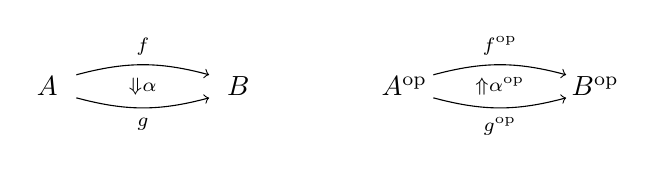
\begin{tikzpicture}[x=1.5em,y=1.3em]
  \node (A) at (0,0) {$A$};
  \node (B) at (4.6,0) {$B$};
  \draw[->] (0.7,0.32) to[bend left=15] node[above,pos=0.5]{$\scriptstyle f$} (3.9,0.32);
  \draw[->] (0.7,-0.32) to[bend right=15] node[below,pos=0.5]{$\scriptstyle g$} (3.9,-0.32);
  \node at (2.3,0) {$\scriptstyle\Downarrow\alpha$};
  \node at (6.6,0) {$\scriptstyle\leftrightsquigarrow$};
  \begin{scope}[shift={(8.6,0)}]
    \node (Ao) at (0,0) {$A^{\mathrm{op}}$};
    \node (Bo) at (4.6,0) {$B^{\mathrm{op}}$};
    \draw[->] (0.7,0.32) to[bend left=15] node[above,pos=0.5]{$\scriptstyle f^{\mathrm{op}}$} (3.9,0.32);
    \draw[->] (0.7,-0.32) to[bend right=15] node[below,pos=0.5]{$\scriptstyle g^{\mathrm{op}}$} (3.9,-0.32);
    \node at (2.3,0) {$\scriptstyle\Uparrow\alpha^{\mathrm{op}}$};
  \end{scope}
\end{tikzpicture}
\end{center}
它是通过施加命题 12.1.5 的拟伪\trFunctor{}所底蕴的那个伪\trFunctor{}
$(-)^{\mathrm{op}}\colon\mathfrak{h}\mathcal{K}\rightsquigarrow\mathfrak{h}\mathcal{K}^{\mathrm{op}}$
而得到的。此外：

\begin{lemma}\label{lem:op-of-cotensor-and-hom}
设 $\mathcal{K}$ 是一个 $(\infty,1)$-\trCategory{}的\trInfinityCosmos。
\begin{enumerate}[label=(\roman*)]
\item 对任何\trInfinityCategory{} $A$ 与\trSimplicialSet{} $U$，有
  $(A^{U})^{\mathrm{op}}\simeq(A^{\mathrm{op}})^{U^{\mathrm{op}}}$。
\item 对任何\trFunctor{} $f\colon B\to A$ 与 $g\colon C\to A$，存在
  $B^{\mathrm{op}}\times C^{\mathrm{op}}$ 之上的一个\trEquivalence
  $\mathrm{Hom}_{A}(f,g)^{\mathrm{op}}\simeq\mathrm{Hom}_{A^{\mathrm{op}}}(g^{\mathrm{op}},f^{\mathrm{op}})$。
\end{enumerate}
\end{lemma}

\begin{proof}
我们有一条拟伪自然的\trEquivalence：
\begin{align*}
\Fun(X,(A^{U})^{\mathrm{op}})
  &\simeq\Fun(X^{\mathrm{op}},A^{U})^{\mathrm{op}}
  &&\text{由 \cref{prop:opposite-quasi-pseudofunctor}}\\
  &\simeq(\Fun(X^{\mathrm{op}},A)^{U})^{\mathrm{op}}
  &&\text{由 \eqref{eq:cotensor-universal}}\\
  &\simeq(\Fun(X^{\mathrm{op}},A)^{\mathrm{op}})^{U^{\mathrm{op}}}
  &&\text{由 \cref{lem:opposite-qcat-biequivalence}}\\
  &\simeq\Fun(X,A^{\mathrm{op}})^{U^{\mathrm{op}}}
  &&\text{由 \cref{prop:opposite-quasi-pseudofunctor}}\\
  &\simeq\Fun(X,(A^{\mathrm{op}})^{U^{\mathrm{op}}})
  &&\text{由 \eqref{eq:cotensor-universal}}.
\end{align*}
故由引理 10.4.14，$(A^{U})^{\mathrm{op}}\simeq(A^{\mathrm{op}})^{U^{\mathrm{op}}}$。

第二个陈述是一个更一般结果的推论：任何拟伪\trFunctor{}性的\trBiequivalence
——例如命题 12.1.5 所确立的
$(-)^{\mathrm{op}}\colon\mathcal{K}\rightsquigarrow\mathcal{K}^{\mathrm{co}}$
——保持并反射诸\trCommaInfinityCategory。或者，由于此处所论的拟伪%
\trFunctor{}性的\trBiequivalence{}定义为诸\trCosmologicalBiequivalence{}的
之字形链，该结果也可由「诸\trCosmologicalBiequivalence{}本身保持并反射诸%
\trCommaInfinityCategory」这一事实——如命题 10.3.6(vi) 所观察到者——得出。
\end{proof}

下一个结果为「诉诸对偶性」提供了另一种视角：此前，关于一个\trInfinityCosmos{}
$\mathcal{K}$ 中诸\trDiagram{}之\trColimit{}的事实，是从关于
$\mathcal{K}^{\mathrm{co}}$ 中诸\trLimit{}的相应证明中演绎而得的；类似地，
关于\trCartesianFibration{}的结果也是在 $\mathcal{K}^{\mathrm{co}}$ 中得到
解读，从而得出关于 $\mathcal{K}$ 中\trCocartesianFibration{}的相应
结果。

\begin{proposition}\label{prop:duality-for-limits-and-fibrations}
设 $\mathcal{K}$ 是一个 $(\infty,1)$-\trCategory{}的\trInfinityCosmos。
\begin{enumerate}[label=(\roman*)]
\item $A$ 中一个 $J$ 形状的图表族拥有一个\trColimit，当且仅当 $A^{\mathrm{op}}$
  中相应的 $J^{\mathrm{op}}$ 形状的图表族拥有一个\trLimit。
\item 一个\trFunctor{} $p\colon E\twoheadrightarrow B$ 定义一个%
  \trCartesianFibration，当且仅当\trFunctor{}
  $p^{\mathrm{op}}\colon E^{\mathrm{op}}\twoheadrightarrow B^{\mathrm{op}}$
  定义一个\trCocartesianFibration。\footnote{正如第三部分的引言中所指出的，
  由 $p^{\mathrm{op}}$ 所编码的同伦相干\trDiagram{}并\emph{不}是由 $p$ 所
  编码的同伦相干\trDiagram{}——这是 Bénabou 的一个经典观察，经 Barwick、
  Glasman 与 Nardin 扩展到 $(\infty,1)$-范畴的语境 $[7]$。}
\end{enumerate}
\end{proposition}

注意：若 $p\colon E\twoheadrightarrow B$ 是一个\trIsofibration，那么总可能
选取一个\trFunctor{}
$p^{\mathrm{op}}\colon E^{\mathrm{op}}\twoheadrightarrow B^{\mathrm{op}}$
使其仍是一个\trIsofibration，或许需要更换全空间 $E^{\mathrm{op}}$ 的选取。

\begin{proof}
由\cref{lem:op-of-cotensor-and-hom}，$A$ 中一个 $J$ 形状的图表族
$d\colon D\to A^{J}$ 定义一个 $J^{\mathrm{op}}$ 形状的图表族
$d^{\mathrm{op}}\colon D^{\mathrm{op}}\to(A^{\mathrm{op}})^{J^{\mathrm{op}}}$。
由命题 4.3.1，%
$d$ 在 $A$ 中容有一个\trColimit，当且仅当存在诸\trCommaInfinityCategory{}的
一个\trEquivalence
\begin{equation*}
\mathrm{Hom}_{A^{J}}(d,\Delta)\simeq_{A\times D}\mathrm{Hom}_{A}(c,A),
\end{equation*}
此时，表示\trFunctor{} $c\colon D\to A$ 定义余极限\trFunctor。

由\cref{lem:op-of-cotensor-and-hom}，这样一个\trEquivalence{}存在，当且仅当
存在一个\trEquivalence
\begin{equation*}
\mathrm{Hom}_{(A^{\mathrm{op}})^{J^{\mathrm{op}}}}(\Delta,d^{\mathrm{op}})
\simeq_{D^{\mathrm{op}}\times A^{\mathrm{op}}}
\mathrm{Hom}_{A^{\mathrm{op}}}(A^{\mathrm{op}},c^{\mathrm{op}}),
\end{equation*}
而由命题 4.3.1，后者刻画了极限\trFunctor{}
$c^{\mathrm{op}}\colon D^{\mathrm{op}}\to A^{\mathrm{op}}$。

第二个陈述类似地证明。由第 5 章中的\cref{thm:internal-characterization}，
$p\colon E\twoheadrightarrow B$ 定义一个\trCartesianFibration，当且仅当受
诱导的\trFunctor{}
$i_{1}\hat{\delta}p\colon E^{2}\twoheadrightarrow\mathrm{Hom}_{B}(B,p)$
容有一个右伴随右逆。施加拟伪\trFunctor{}性的\trBiequivalence{}
$(-)^{\mathrm{op}}\colon\mathcal{K}\rightsquigarrow\mathcal{K}^{\mathrm{co}}$，
这个\trAdjunction{}存在，当且仅当那个反\trFunctor{}容有一个左伴随右逆。这个%
\trFunctor{}未必\trIsomorphism{}于
$i_{0}\hat{\delta}p^{\mathrm{op}}\colon(E^{\mathrm{op}})^{2}\twoheadrightarrow\mathrm{Hom}_{B^{\mathrm{op}}}(p^{\mathrm{op}},B^{\mathrm{op}})$，
但由\cref{lem:op-of-cotensor-and-hom}它与后者\trEquivalence{}，而由伴随的%
\trEquivalence{}不变性，这就足够了（见练习 B.4.i）。由第 5 章中的%
\cref{thm:internal-characterization}的对偶，这样一个\trAdjunction{}存在，
当且仅当 $p^{\mathrm{op}}\colon E^{\mathrm{op}}\twoheadrightarrow B^{\mathrm{op}}$
是一个\trCocartesianFibration。
\end{proof}

我们现在把注意力转向一个\trQuasiCategory{}的 Kan 复形核的构造，并讨论其在
其他 $(\infty,1)$-\trCategory{}的\trInfinityCosmos{}中的类比。

\begin{definition}\label{def:infinity-groupoid-core-quasi-category}
一个\trQuasiCategory{} $A$ 的\textbf{\trInfinityGroupoidCore}（∞-groupoid
core）是最大的\trKanComplex{} $\mathrm{core}A\subseteq A$，它可构造为包含
下列成分的单纯子集：
\begin{itemize}
\item $A$ 的全部顶点；
\item 恰那些在 $A$ 中定义\trIsomorphism{}的边（见第 1 章中的%
  \cref{def:isomorphism-quasi-category}）；
\item 每条边皆为\trIsomorphism{}的更高维单纯形。
\end{itemize}
\end{definition}

\begin{lemma}\label{lem:core-is-kan-complex}
一个\trQuasiCategory{}的\trInfinityGroupoidCore{}是一个\trKanComplex，而且
它确实是含于该\trQuasiCategory{} $A$ 之中的最大\trKanComplex。
\end{lemma}

\begin{proof}
\cref{def:infinity-groupoid-core-quasi-category}中所构造的包含 $\mathrm{core}A\subset A$ 在除维数一以外的所有
维数的单纯形上都是满的。于是，为见 $\mathrm{core}A$ 是一个\trQuasiCategory，
只需论证它沿\trHorn{} $\Lambda^{1}[2]\hookrightarrow\Delta[2]$ 容有%
\trExtension。由构造，一支\trHorn{} $\Lambda^{1}[2]\to\mathrm{core}A$ 选取出
$A$ 中的两个\trIsomorphism。填充体 $\Delta[2]\to A$ 见证\trHomotopyCategory{}
$\mathrm{h}A$ 中的一个复合关系；于是该复合边也是\trIsomorphism，且由满性，
这个填充体提升为 $\Delta[2]\to\mathrm{core}A$。

由构造，$\mathrm{h}(\mathrm{core}A)$ 是一个\trGroupoid；而且它是含于
$\mathrm{h}A$ 中的极大子\trGroupoid。于是由第 1 章中的\cref{cor:kan-groupoid}，
$\mathrm{core}A$ 是一个\trKanComplex。

最后，一个中间单纯子集 $\mathrm{core}A\subsetneq K\subset A$ 必然包含一条
额外的边 $f\colon x\to y$。若 $K$ 是一个\trKanComplex，则它必须对
$\Lambda^{0}[2]$-号角与 $\Lambda^{2}[2]$-号角容有填充体：其第 2 个面与第 0
个面（视情形）为该 1-\trSimplex{} $f$，而其余那个面是退化的。这些填充体会在
$\mathrm{h}(A)$ 中构造出 $f$ 的左逆与右逆。于是，$f$ 是 $A$ 中的一个%
\trIsomorphism，从而已居于 $\mathrm{core}A$ 之中。
\end{proof}

\trKanComplex{}的\trInfinityCosmos{}的包含定义了一个\trCosmologicalEmbedding{}
$\Kan\hookrightarrow\QCat$，依据是第 6 章中的\cref{prop:discrete-cosmos}。
诸\trQuasiCategory{}之间的\trFunctor{}保持\trIsomorphism，于是一个%
\trFunctor{} $f\colon A\to B$ 限制为\trFunctor{}
$f\colon\mathrm{core}A\to\mathrm{core}B$。如此，\trInfinityGroupoidCore{}%
构造在 $\QCat$ 的底\trCategory{}上函子式地作用，并且作为一个非富集的%
\trFunctor{}，它是这个包含的\trRightAdjoint。然而，正如第 1 章中的%
\cref{exa:core-not-cosmological}所讨论的，核构造不是单纯的，至少相对于
$\QCat$ 的通常拟范畴式富集而言不是。的确，诸\trQuasiCategory{}之间的%
\trFunctor{}之间的一个\trNaturalTransformation{}只有在其各分量都可逆时才
限制到诸\trInfinityGroupoidCore{}上。

然而，\trInfinityGroupoidCore{}确实相对于我们现在引入的一种新富集定义一个%
\trSimplicialFunctor。一个\trInfinityCosmos{}是 $(\infty,2)$-\trCategory{}%
的一种类型，因为它是一个富集于 $(\infty,1)$-\trCategory{}的某个模型之上的%
\trCategory。我们现在引入一个\trInfinityCosmos{}的
$(\infty,1)$-\textbf{范畴核}（$(\infty,1)$-categorical core）。在下面的
定义中，注意：由于 $\mathrm{core}(-)\colon\QCat\to\Kan$ 是一个（非富集的）
右伴随，它保持乘积，故我们可以把它施加于一个以拟范畴富集的\trCategory{}的
诸\trFunctorSpace{}之上，以构造一个 Kan 复形富集子\trCategory{}（见命题
A.7.3），我们现在就来引入。

\begin{definition}[一个\trInfinityCosmos{}的 $(\infty,1)$-核]\label{def:infinity-one-core-cosmos}
对一个\trInfinityCosmos{} $\mathcal{K}$，记 $\coreS\mathcal{K}\subset\mathcal{K}$
为与之具有相同对象的子\trCategory，其内部 hom 定义为 $\mathcal{K}$ 的诸%
\trFunctorSpace{}的诸\trInfinityGroupoidCore。我们把 $\coreS\mathcal{K}$
称为 $\mathcal{K}$ 的 \textbf{$(\infty,1)$-核}，并把它设想为居于这个
$(\infty,2)$-\trCategory{}内部的核心 $(\infty,1)$-\trCategory。
\end{definition}

\begin{remark}\label{rem:core-not-infinity-cosmos}
$(\infty,1)$-范畴核不是在第 1 章中的\cref{def:infinity-cosmos}所公理化的
严格意义下的一个\trInfinityCosmos。它从原来的\trInfinityCosmos{}继承了其%
\trIsofibration{}类与诸\trCone{}形\trLimit{}，但单纯\trCotensor{}只是弱式地
存在：$\coreS\mathcal{K}$ 中一个\trInfinityCategory{} $A$ 由一个%
\trSimplicialSet{} $U$ 所作的\trCotensor，经由 $\mathcal{K}$ 中 $A$ 与 $U$
的一个 Kan 复形替换 $\bar{U}$ 的\trCotensor{}来构造，其中 $\bar{U}$ 由
「自由可逆化」其诸边并为诸\trHorn{}添加填充体而定义。其结果是一个%
\trEquivalence{}
$\mathrm{core}(\Fun(X,A)^{U})\simeq\mathrm{core}(\Fun(X,A^{\bar{U}}))$，
用以取代通常的\trIsomorphism。或者，\cref{ex:marked-enrichment-core}提示了
另一种进路来定义一个\trInfinityCosmos{}的富集，使得 $(\infty,1)$-核仍是
一个\trInfinityCosmos。
\end{remark}

\begin{lemma}\label{lem:kan-inclusion-factors-through-core}
自然包含 $\Kan\hookrightarrow\QCat$ 经由包含 $\coreS\QCat\subset\QCat$ 而
分解，且后一\trFunctor{}容有一个单纯富集的右伴随左逆，亦即把每个%
\trQuasiCategory{}送到其\trInfinityGroupoidCore{}的那个\trFunctor：
\begin{center}
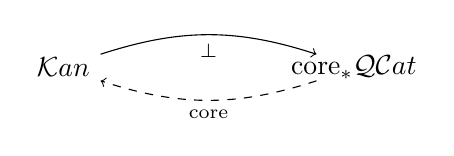
\begin{tikzpicture}[x=1.5em,y=1.2em]
  \node (Kan) at (0,0) {$\Kan$};
  \node (CQ)  at (7.0,0) {$\coreS\QCat$};
  \draw[->] (0.9,0.4) to[bend left=18] node[midway,below]{$\scriptstyle\perp$} (6.1,0.4);
  \draw[->,dashed] (6.1,-0.4) to[bend left=18] node[midway,below]{$\scriptstyle\mathrm{core}$} (0.9,-0.4);
\end{tikzpicture}
\end{center}
\end{lemma}

\begin{proof}
若 $K$ 与 $L$ 是\trKanComplex，则 $\Fun(K,L)$ 亦是。于是自然包含
$\Kan\hookrightarrow\QCat$ 经由 $(\infty,1)$-范畴核而分解。

右伴随 $\mathrm{core}\colon\coreS\QCat\to\QCat$ 在对象上按\cref{def:infinity-groupoid-core-quasi-category}的
构造作用。为定义其在诸\trFunctorSpace{}上的作用，我们必须对任何一对%
\trQuasiCategory{} $A$ 与 $B$ 提供一个典范映射
\begin{equation*}
\mathrm{core}(\Fun(A,B))\to\Fun(\mathrm{core}A,\mathrm{core}B)
\end{equation*}
由第 1 章中的\cref{cor:exponential-ideal}，$\Fun(A,B)\cong B^{A}$ 中的诸%
\trIsomorphism{}恰是那些单纯映射 $\alpha\colon A\times\Delta[1]\to B$：其
由 $A$ 的顶点 $a$ 标引的诸分量 $\alpha_{a}\colon\Delta[1]\to B$ 定义 $B$ 中
的\trIsomorphism。把这一观察与\cref{def:infinity-groupoid-core-quasi-category}相结合，我们看到
$\mathrm{core}(\Fun(A,B))$ 中的一个 $n$-单纯形是一个单纯映射
$\phi\colon A\times\Delta[n]\to B$，它具有如下性质：限制到 $A$ 的任何顶点与
$\Delta[n]$ 的任何边上时，所得 $B$ 中的边是一个\trIsomorphism。当 $A$ 限制
到其\trKanComplex{}核时，$\mathrm{core}A$ 的边也是\trIsomorphism。于是
$\phi\colon\mathrm{core}A\times\Delta[n]\to B$ 把定义域的每条边送到 $B$ 中
的一个\trIsomorphism，从而经由 $\mathrm{core}B\hookrightarrow B$ 分解，
因为这个包含在可逆的边上是满的。\footnote{在带标记单纯集的语言中，
$\mathrm{core}(\Fun(A,B))$ 中的一个映射是一个带标记映射
$A^{\sharp}\times\Delta[n]^{\sharp}\to B^{\flat}$。沿
$\mathrm{core}A^{\sharp}\hookrightarrow A^{\sharp}$ 限制后，定义域
$\mathrm{core}A^{\sharp}\times\Delta[n]^{\sharp}$ 是极大标记的，从而经由
极大标记的 $\mathrm{core}B^{\flat}\hookrightarrow B^{\flat}$ 分解（见 D.4
节）。}于是，这个 $n$-单纯形 $\phi$ 限制而定义一个 $n$-单纯形
$\phi\colon\mathrm{core}A\times\Delta[n]\to\mathrm{core}B$。这就定义了该
典范映射。

现在，对一个\trKanComplex{} $K$ 与一个\trQuasiCategory{} $A$，单纯自然%
\trIsomorphism
\begin{equation*}
\mathrm{core}(\Fun(K,A))\cong\Fun(K,\mathrm{core}A)
\end{equation*}
是易于验证的。顶点上的对应表达了非富集的\trAdjunction，而更高维单纯形上的
对应则循刚才讨论的理由以及\trIsomorphism{} $\mathrm{core}(K)\cong K$ 而得。
\end{proof}

\begin{corollary}\label{cor:core-of-equivalent-quasi-categories}
若 $A$ 与 $B$ 是\trEquivalence{}的\trQuasiCategory，则 $\mathrm{core}A$ 与
$\mathrm{core}B$ 是\trEquivalence{}的\trKanComplex。
\end{corollary}

\begin{proof}
诸\trQuasiCategory{}之间的一个\trEquivalence{}由一对 $0$-箭头连同可逆
$1$-箭头的一对所指定。如此，它包含于 $(\infty,1)$-范畴核
$\coreS\QCat\hookrightarrow\QCat$ 之中，并被\trSimplicialFunctor{}
$\mathrm{core}\colon\coreS\QCat\to\Kan$ 所保持。
\end{proof}

一个 $(\infty,1)$-\trCategory{}的一般\trInfinityCosmos{}中的一个%
\trInfinityCategory{}的核，可以按与\cref{def:opposite-infinity-category}类似的方式定义，但这个概念
还拥有一个到\trEquivalence{}为止的\trUniversalProperty，我们更愿意把它用作
定义。

\begin{definition}\label{def:infinity-groupoid-core-cosmos}
设 $\mathcal{K}$ 是一个 $(\infty,1)$-\trCategory{}的\trInfinityCosmos{}，
并设 $A$ 是 $\mathcal{K}$ 中的一个\trInfinityCategory。它的%
\textbf{\trInfinityGroupoidCore}是一个配有映射 $\iota\colon\mathrm{core}A\to A$
的\trInfinityCategory{} $\mathrm{core}A$，使得
\begin{itemize}
\item $\mathrm{core}A$ 是一个\trDiscrete{}\trInfinityCategory——意即对
  一切 $X$，$\Fun(X,\mathrm{core}A)$ 是一个\trKanComplex；%
  \footnote{原书此处印作「meaning that $\Fun(X,A)$ is a Kan complex for all
  $X$」。按本条首句所断言者乃 $\mathrm{core}A$ 之离散性，而\trDiscrete{}%
  \trInfinityCategory{}之定义（第 1 章中的\cref{def:discrete-infinity-categories}）
  正是「对一切 $X$，$\Fun(X,-)$ 皆为\trKanComplex」，故疑为
  $\Fun(X,\mathrm{core}A)$ 之误，此处径改。——译者注}
\item 若 $G$ 是一个\trDiscrete{}\trInfinityCategory，则 $\iota$ 定义一个%
  \trEquivalence
\begin{equation*}
\Fun(G,\mathrm{core}A)\xrightarrow{\ \iota\circ-\ }\mathrm{core}(\Fun(G,A))
\end{equation*}
\end{itemize}
\end{definition}

在实践中，一个 $(\infty,1)$-\trCategory{}的\trInfinityCosmos{}常常配有一个
显式的\trCoreFunctor{}；但与反者的情形一样，它也可以经由一个合适的%
\trChangeOfModel{}\trFunctor{}搬运核构造而定义：

\begin{proposition}\label{prop:core-quasi-pseudofunctor}
在一个 $(\infty,1)$-\trCategory{}的\trInfinityCosmos{} $\mathcal{K}$ 中，
任何一组对∞-\trInfinityGroupoidCore{}的选取都装配成一个拟伪\trFunctor{}
$\mathrm{core}\colon\coreS\mathcal{K}\to\Disc(\mathcal{K})$。特别地，对任意%
\trInfinityCategory{} $A,B\in\mathcal{K}$，存在一个映射
$\mathrm{core}(\Fun(A,B))\to\Fun(\mathrm{core}A,\mathrm{core}B)$，它在 $A$
与 $B$ 上（作为 $\coreS\mathcal{K}$ 的对象）都是拟伪自然的。
\end{proposition}

\begin{proof}
该拟伪\trFunctor{}定义为某个之字形链的复合，其中逆向的映射是一个%
\trCosmologicalBiequivalence，依据是推论 10.3.7：
\begin{center}
\begin{tikzpicture}[x=1.7em,y=1.5em]
  \node (tl) at (0,1.6) {$\coreS\mathcal{K}$};
  \node (tr) at (6.4,1.6) {$\Disc(\mathcal{K})$};
  \draw[->] (1.1,1.6) -- ++(0.60,0.07) -- ++(0.60,-0.14) -- ++(0.60,0.14)
    -- ++(0.60,-0.14) -- ++(0.60,0.14) -- ++(0.60,-0.14) -- ++(0.60,0.07);
  \node at (3.2,2.0) {$\scriptstyle\mathrm{core}(-)$};
  \draw[right hook->] (0,1.1) -- (0,0.45);
  \node at (-0.9,0.78) {$\scriptstyle(-)_{0}$};
  \node at (3.2,0.78) {$\scriptstyle\cong$};
  \draw[right hook->] (6.4,1.1) -- (6.4,0.45);
  \node at (7.3,0.78) {$\scriptstyle(-)_{0}$};
  \node (bl) at (0,0) {$\coreS\QCat$};
  \node (br) at (6.4,0) {$\Kan\cong\Disc(\QCat)$};
  \draw[->] (1.5,0) -- node[above]{$\scriptstyle\sim$}
    node[below]{$\scriptstyle\mathrm{core}(-)$} (3.9,0);
\end{tikzpicture}
\end{center}
我们把「$\mathcal{K}\rightsquigarrow\mathcal{L}$ 下降为一个单纯富集的%
\trBiequivalence{} $\coreS\mathcal{K}\rightsquigarrow\coreS\mathcal{L}$」的验证
留给\cref{ex:core-functor-biequivalence}。由命题 10.4.16，%
宇宙论\trBiequivalence{} $(-)_{0}\colon\Disc(\mathcal{K})\Rightarrow\Kan$
的逆定义一个拟伪\trFunctor{}与\trBiequivalence{}
$\Kan\rightsquigarrow\Disc(\mathcal{K})$，后者与单纯\trFunctor{}
$\mathrm{core}((-)_{0})\colon\coreS\mathcal{K}\to\Kan$ 相复合而定义拟伪%
\trFunctor{} $\mathrm{core}\colon\coreS\mathcal{K}\to\Disc(\mathcal{K})$。
由引理 10.4.12，这个拟伪\trFunctor{}在各 hom 上的作用定义一个拟伪自然变换。

尚待验证的只是：该拟伪\trFunctor{}在对象上的作用满足\cref{def:infinity-groupoid-core-cosmos}
的诸条件。由构造，对任何 $A\in\mathcal{K}$，$\mathrm{core}A$ 是一个%
\trDiscrete{}\trInfinityCategory。映射 $\iota\colon\mathrm{core}A\to A$
定义为把「\trQuasiCategory{}的\trKanComplex{}核的相应包含」与「底%
\trQuasiCategory{}\trFunctor{}及其拟伪\trFunctor{}性的逆」作须化：
\begin{equation*}
\coreS\mathcal{K}\;\xrightarrow[\ \sim\ ]{(-)_{0}}\;\coreS\QCat\;\;
\overset{\mathrm{core}}{\underset{\hookrightarrow}{\rightleftarrows}}\;\;
\coreS\QCat\;\overset{(-)_{0}^{-1}}{\rightsquigarrow}\;\coreS\mathcal{K}
\end{equation*}
现在，若 $G$ 是一个\trDiscrete{}\trInfinityCategory，则
$G_{0}=\Fun(1,G)$ 是一个\trKanComplex，于是由\cref{lem:kan-inclusion-factors-through-core}，
$\iota_{A_{0}}\circ-\colon\Fun(G_{0},\mathrm{core}(A_{0}))\rightsquigarrow\mathrm{core}(\Fun(G_{0},A_{0}))$
是一个\trEquivalence。由构造，$\mathrm{core}A$ 定义成使得
$(\mathrm{core}A)_{0}\cong\mathrm{core}(A_{0})$。注意：由于
$(-)_{0}\colon\mathcal{K}\Rightarrow\QCat$ 是一个\trBiequivalence，这表明：
一个 $(\infty,1)$-\trCategory{}的\trInfinityCosmos{}中的一个%
\trInfinityCategory{}的核在\trEquivalence{}意义下是良定义的。由于单纯%
\trFunctor{} $(-)_{0}\colon\coreS\mathcal{K}\to\coreS\QCat$ 在各 hom 上是%
\trEquivalence，由与 $\iota_{A}$ 作后复合所定义的\trFunctor{}等价于这个%
\trFunctor
\begin{center}
\begin{tikzpicture}[x=1.6em,y=1.5em]
  \node (tl) at (0,1.6) {$\Fun(G,\mathrm{core}A)$};
  \node (tr) at (7.0,1.6) {$\mathrm{core}(\Fun(G,A))$};
  \draw[->] (tl) -- node[above]{$\scriptstyle\iota_{A}\circ-$} (tr);
  \draw[right hook->] (0,1.1) -- (0,0.45);
  \node at (-0.9,0.78) {$\scriptstyle(-)_{0}$};
  \node at (3.5,0.78) {$\scriptstyle\cong$};
  \draw[right hook->] (7.0,1.1) -- (7.0,0.45);
  \node at (7.9,0.78) {$\scriptstyle(-)_{0}$};
  \node (bl) at (0,0) {$\Fun(G_{0},\mathrm{core}A_{0})$};
  \node (br) at (7.0,0) {$\mathrm{core}(\Fun(G_{0},A_{0}))$};
  \draw[->] (bl) -- node[above]{$\scriptstyle\sim$}
    node[below]{$\scriptstyle\iota_{A_{0}}\circ-$} (br);
\end{tikzpicture}
\end{center}
于是，与 $\iota_{A}$ 的后复合诱导所需的\trEquivalence{}
$\Fun(G,\mathrm{core}A)\cong\mathrm{core}(\Fun(G,A))$，证明完成。
\end{proof}

\subsection*{练习}

\begin{exercise}\label{ex:homotopy-category-of-opposite}
证明：一个\trInfinityCategory{} $A$ 之反者的\trHomotopyCategory\trEquivalence{}%
于 $A$ 的\trHomotopyCategory{}之反者。
\end{exercise}

\begin{exercise}\label{ex:opposite-of-equivalence}
证明：诸\trInfinityCategory{}之间的一个\trFunctor{}是一个\trEquivalence，
当且仅当其反\trFunctor{}是一个\trEquivalence。
\end{exercise}

\begin{exercise}\label{ex:marked-enrichment-core}
在 D.4 节与 D.5 节的协助下：
\begin{enumerate}[label=(\roman*)]
\item 重新定义第 1 章中的\cref{def:infinity-cosmos}的\trInfinityCosmos{}%
  概念，使之成为一个富集于带标记单纯集之上的\trCategory{}，其诸%
  \trFunctorSpace{}为自然标记的\trQuasiCategory。
\item 描述带这种富集的\trInfinityCosmos{}中、一个自然标记的%
  \trQuasiCategory{}的\trInfinityGroupoidCore{}以及一个\trInfinityCosmos{}%
  的 $(\infty,1)$-范畴核的构造。
\item 证明 $(\infty,1)$-范畴核与单纯集作余张量，尽管这些\trCotensor{}并不
  被包含 $\coreS\mathcal{K}\hookrightarrow\mathcal{K}$ 所保持。
\item 证明一个\trInfinityCosmos{}的 $(\infty,1)$-核是新意义下的一个%
  \trInfinityCosmos{}，尽管\trFunctor{}
  $\coreS\mathcal{K}\hookrightarrow\mathcal{K}$ 仍不是宇宙论的。
\end{enumerate}
\end{exercise}

\begin{exercise}\label{ex:core-functor-biequivalence}
设 $F\colon\mathcal{K}\to\mathcal{L}$ 是一个\trCosmologicalFunctor。证明：
$F$ 诱导一个单纯\trFunctor{} $F\colon\coreS\mathcal{K}\to\coreS\mathcal{L}$，
并且若原来的\trFunctor{}是一个\trBiequivalence，则它也是一个\trBiequivalence。
\end{exercise}

\begin{exercise}\label{ex:adjunction-restricts-adjoint-equivalence}
\begin{enumerate}[label=(\roman*)]
\item 证明：诸\trQuasiCategory{}之间的任何\trAdjunction
\begin{center}
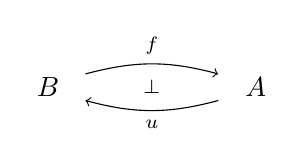
\begin{tikzpicture}[x=1.5em,y=1.2em]
  \node (B) at (0,0) {$B$};
  \node (A) at (5.0,0) {$A$};
  \draw[->] (0.9,0.4) to[bend left=15] node[above,pos=0.5]{$\scriptstyle f$} (4.1,0.4);
  \node at (2.5,0) {$\scriptstyle\perp$};
  \draw[->] (4.1,-0.4) to[bend left=15] node[below,pos=0.5]{$\scriptstyle u$} (0.9,-0.4);
\end{tikzpicture}
\end{center}
都限制而定义一个介于诸全子拟范畴之间的伴随\trEquivalence——这些全子拟范畴
由那些使单位与余单位分量（各自地）可逆的\trElement{} $b\colon 1\to B$ 与
$a\colon 1\to A$ 张成。
\item 陈述并证明一个关于伴随\trEquivalence{}的类似结果，其中的伴随%
\trEquivalence{}由任意一个 $(\infty,1)$-\trCategory{}的\trInfinityCosmos{}%
中的诸\trAdjunction{}导出。
\end{enumerate}
\end{exercise}

   %

\providecommand{\Fun}{\operatorname{Fun}}
\providecommand{\QCat}{\mathcal{Q}\mathcal{C}at}
\providecommand{\qcor}[1]{\ulcorner#1\urcorner}   %
\providecommand{\qcInt}{\mathbb{I}}   %
\providecommand{\PUpair}[5]{\tikz[baseline=-0.6ex,x=1.15em,y=0.95em]{%
  \node (PUa) at (0,0) {$#1$};%
  \node (PUb) at (3.6,0) {$#2$};%
  \draw[->] (0.65,0.38) to[bend left=12] node[above]{$\scriptstyle#3$} (2.95,0.38);%
  \node at (1.8,0) {$\scriptstyle\Downarrow#4$};%
  \draw[->] (0.65,-0.38) to[bend right=12] node[below]{$\scriptstyle#5$} (2.95,-0.38);}}

\section{逐点泛性质}\label{sec:pointwise-universal-properties}

在一个 $(\infty,1)$-\trCategory{}的\trInfinityCosmos{}中，\trTerminal{}%
∞-\trCategory{} $1$ 扮演着一个特殊角色，这一角色可以概括为如下口号：%
「诸\trUniversalProperty{}是逐点检测的」。在本节中，我们汇集起若干例示这一
口号的结果，它们的证明综合运用了综合技巧与解析技巧。

例如，第 1 章中的\cref{cor:exponential-ideal}陈述而附录 D 的推论 D.4.19 证明：%
诸\trQuasiCategory{}之间的诸\trFunctor{}之间的一个\trNaturalTransformation{}
\PUpair{X}{A}{f}{\alpha}{g}是一个自然同构，当且仅当它是一个\textbf{逐点同构}
（pointwise isomorphism），意即它的每一个分量
\tikz[baseline=-0.6ex,x=1.15em,y=0.95em]{%
  \node (PUa) at (0,0) {$1$};%
  \node (PUb) at (3.6,0) {$X$};%
  \node (PUc) at (7.2,0) {$A$};%
  \draw[->] (PUa) -- node[above]{$\scriptstyle x$} (PUb);%
  \draw[->] (4.25,0.38) to[bend left=12] node[above]{$\scriptstyle f$} (6.55,0.38);%
  \node at (5.4,0) {$\scriptstyle\Downarrow\alpha$};%
  \draw[->] (4.25,-0.38) to[bend right=12] node[below]{$\scriptstyle g$} (6.55,-0.38);}
是可逆的。从而：

\begin{lemma}\label{lem:pointwise-natural-isomorphism}
在一个 $(\infty,1)$-\trCategory{}的\trInfinityCosmos{}中，一个%
\trNaturalTransformation{}是一个自然同构，当且仅当它是一个逐点同构。
\end{lemma}

\begin{proof}
任何自然同构显然都是逐点同构。为证其逆，我们动用命题 10.2.1 与命题 10.3.1 的
2-范畴双等价 $(-)_{0}\colon\mathfrak{h}\mathcal{K}\Rightarrow\mathfrak{h}\QCat$。
设 \PUpair{X}{A}{f}{\alpha}{g} 是 $\mathfrak{h}\mathcal{K}$ 中的一个逐点自然
同构，并考虑诸底拟范畴之间的底\trNaturalTransformation{}
\PUpair{X_{0}}{A_{0}}{f_{0}}{\alpha_{0}}{g_{0}}。由构造，$X_{0}\cong\Fun(1,X)$
的顶点 $x$ 与 $X$ 的诸\trElement{}双射地对应，而这些分量
\begin{center}
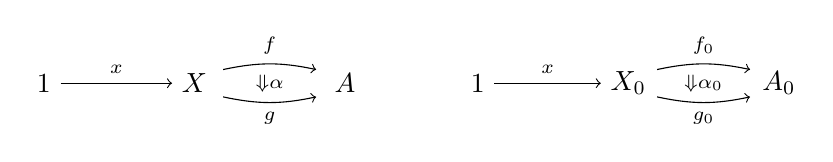
\begin{tikzpicture}[x=1.6em,y=1.3em]
  \node (a1) at (0,0) {$1$};
  \node (b1) at (3.4,0) {$X$};
  \node (c1) at (6.8,0) {$A$};
  \draw[->] (a1) -- node[above]{$\scriptstyle x$} (b1);
  \draw[->] (4.05,0.38) to[bend left=12] node[above]{$\scriptstyle f$} (6.15,0.38);
  \node at (5.1,0) {$\scriptstyle\Downarrow\alpha$};
  \draw[->] (4.05,-0.38) to[bend right=12] node[below]{$\scriptstyle g$} (6.15,-0.38);
  \node at (8.3,0) {$\leftrightsquigarrow$};
  \begin{scope}[shift={(9.8,0)}]
    \node (a2) at (0,0) {$1$};
    \node (b2) at (3.4,0) {$X_{0}$};
    \node (c2) at (6.8,0) {$A_{0}$};
    \draw[->] (a2) -- node[above]{$\scriptstyle x$} (b2);
    \draw[->] (4.05,0.38) to[bend left=12] node[above]{$\scriptstyle f_{0}$} (6.15,0.38);
    \node at (5.1,0) {$\scriptstyle\Downarrow\alpha_{0}$};
    \draw[->] (4.05,-0.38) to[bend right=12] node[below]{$\scriptstyle g_{0}$} (6.15,-0.38);
  \end{scope}
\end{tikzpicture}
\end{center}
在 $\mathrm{h}A\cong\mathrm{h}(A_{0})$ 中定义相应的箭头。于是，底%
\trNaturalTransformation{} $\alpha_{0}$ 在 $\mathfrak{h}\QCat$ 中也是一个逐点
自然同构，而推论 D.4.19 适用于证明 $\alpha_{0}$ 容有一个逆
\PUpair{X_{0}}{A_{0}}{g_{0}}{\alpha_{0}^{-1}}{f_{0}}。由命题 10.3.1 所建立的
局部等价 $\mathrm{h}\Fun(X,A)\Rightarrow\mathrm{h}\Fun(X_{0},A_{0})$ 的
全忠实性，这个 2-胞腔提升而定义一个逆\trNaturalTransformation{}
\PUpair{X}{A}{g}{\alpha^{-1}}{f}，见证 $\alpha$ 的可逆性。
\end{proof}

值得提请注意：\cref{lem:pointwise-natural-isomorphism}之证明中所用的宇宙论%
\trBiequivalence{} $(-)_{0}\colon\mathcal{K}\Rightarrow\QCat$ 的一个特殊性质。

\begin{observation}[论底拟范畴的\trElement]\label{obs:elements-of-underlying-qcat}
由推论 10.3.2(ii)，一个宇宙论\trBiequivalence{}
$F\colon\mathcal{K}\Rightarrow\mathcal{L}$ 在 $\mathcal{K}$ 中一个%
∞-\trCategory{} $A\in\mathcal{K}$ 的诸\trElement{}的同构类与 $\mathcal{L}$ 中
$FA\in\mathcal{L}$ 的诸\trElement{}的同构类之间诱导一个双射，而且事实上诱导%
诸\trHomotopyCategory{}的一个\trEquivalence{} $\mathrm{h}A\Rightarrow\mathrm{h}FA$
——后者的对象恰是这些元素（见练习 10.3.i）。特别地，任何\trElement{}
$x\colon 1\to FA$ 都自然同构于一个\trElement{} $Fa\colon 1\to FA$，后者是某个%
\trElement{} $a\colon 1\to A$ 的像。由于「逐点的」∞-范畴性概念——一个自然
同构诸分量的可逆性、一个\trCocartesianFibration{}诸纤维中\trTerminal{}元素
之拥有——在\trIsomorphism{}之下不变，故若 $A$ 在 $\mathcal{K}$ 中满足某个逐点
判据，则 $FA$ 在 $\mathcal{L}$ 中满足相应的逐点判据。
\end{observation}

但在 $(\infty,1)$-\trCategory{}的\trInfinityCosmos{}的情形中，命题 10.2.1 提供了一个宇宙论%
\trBiequivalence{} $(-)_{0}\colon\mathcal{K}\to\QCat$，它在∞-%
\trCategory{}的诸\trElement{}上双射地作用。由构造，$A_{0}\cong\Fun(1,A)$ 的
诸顶点与 $A$ 的诸\trElement{}双射地对应。从而，正如%
\cref{lem:pointwise-natural-isomorphism}之证明所例示的，「逐点的」性质甚至可
以更容易地转移。

借助\cref{lem:pointwise-natural-isomorphism}，我们可以证明：一个 $(\infty,1)$-%
\trCategory{}的\trInfinityCosmos{}中的一个\trIsofibration{}是\trSliceInfinityCosmos{}中的一个\trDiscrete{}对象，当且仅当它的诸纤维是\trDiscrete{}%
∞-\trCategory。由此可知：$(\infty,1)$-\trCategory{}的\trCocartesianFibration、%
\trCartesianFibration{}或\trTwoSidedFibration{}是\trDiscrete，当且仅当它们
拥有\trDiscrete{}纤维。

\begin{proposition}\label{prop:discrete-fibers-isofibration}
设 $p\colon E\twoheadrightarrow B$ 是一个 $(\infty,1)$-\trCategory{}的%
\trInfinityCosmos{} $\mathcal{K}$ 中的一个\trIsofibration。则 $p$ 作为
$\mathcal{K}_{/B}$ 的对象是\trDiscrete，当且仅当 $p$ 的诸纤维是 $\mathcal{K}$
中的\trDiscrete{}∞-\trCategory。
\end{proposition}

\begin{proof}
任何\trElement{} $b\colon 1\to B$ 诱导一个宇宙论\trFunctor{}
$b^{*}\colon\mathcal{K}_{/B}\to\mathcal{K}$，由第 1 章中的%
\cref{rem:cosmological-discrete-categories}它保持\trDiscrete{}∞-\trCategory。
于是，对任何\trInfinityCosmos{} $\mathcal{K}$，若
$p\colon E\twoheadrightarrow B$ 是 $\mathcal{K}_{/B}$ 中一个\trDiscrete{}%
对象，则它的诸纤维是\trDiscrete{}∞-\trCategory。

为证其逆，我们假设 $\mathcal{K}$ 是一个 $(\infty,1)$-\trCategory{}的%
\trInfinityCosmos{}并诉诸\cref{lem:pointwise-natural-isomorphism}。为证
$p\colon E\twoheadrightarrow B$ 在 $\mathcal{K}_{/B}$ 中是\trDiscrete，
我们必须论证：由如下\trPullback{}所定义的\trQuasiCategory
\begin{center}
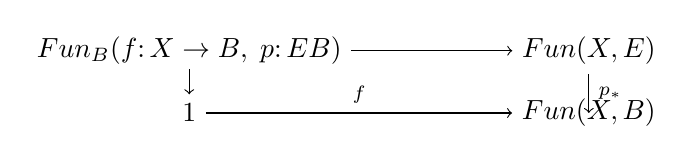
\begin{tikzpicture}[x=1.9em,y=1.5em]
  \node (tl) at (0,1.5) {$\Fun_{B}(f\colon X\to B,\; p\colon E\twoheadrightarrow B)$};
  \node (tr) at (7.6,1.5) {$\Fun(X,E)$};
  \node (bl) at (0,0) {$1$};
  \node (br) at (7.6,0) {$\Fun(X,B)$};
  \draw[->] (tl) -- (tr);
  \draw[->] (0,1.05) -- (0,0.45);
  \draw[->] (tr) -- node[right]{$\scriptstyle p_{*}$} (tr |- br);
  \draw[->] (bl) -- node[above]{$\scriptstyle f$} (br);
  \node at (1.15,0.95) {$\scriptstyle\lrcorner$};
\end{tikzpicture}
\end{center}
是一个\trKanComplex。由第 1 章中的\cref{cor:kan-groupoid}，只需证明其%
\trHomotopyCategory{}是一个\trGroupoid；为此我们动用第 3 章中的%
\cref{lem:smothering-pullback}的\trSmotheringFunctor
\[
\mathrm{h}\bigl(\Fun_{B}(f\colon X\to B,\; p\colon E\twoheadrightarrow B)\bigr)
  \longrightarrow 1\times_{\mathrm{h}\Fun(X,B)}\mathrm{h}\Fun(X,E)
\]
它特别地反射诸\trIsomorphism。$\mathrm{h}(\Fun_{B}(f,p))$ 的诸箭头由那些具有
如下性质的 1-\trSimplex{} $\alpha\colon e\to e'\in\Fun(X,E)$ 所表示：须化复合
$p\alpha\in\Fun(X,B)$ 是 $f$ 处的退化 1-\trSimplex。\footnote{这蕴含、但强于
如下性质：\trHomotopyTwoCategory{}中的须化复合等于 2-\trCell{} $\mathrm{id}_{f}$
（讨论见 3.6 节）。}由\cref{lem:pointwise-natural-isomorphism}，%
\trNaturalTransformation{} $\alpha\colon e\Rightarrow e'\in\mathrm{h}\Fun(X,E)$
是可逆的，当且仅当其对每个 $x\colon 1\to X$ 的分量 $\alpha_{x}$ 都是可逆的。
由于 1-\trSimplex{} $p\alpha$ 在 $\Fun(X,B)$ 中退化，1-\trSimplex{} $p\alpha_{x}$
在顶点 $fx\in\Fun(1,B)$ 处退化，这表明 $\alpha_{x}$ 落于 $fx\colon 1\to B$
之上的纤维中。由于 $p\colon E\twoheadrightarrow B$ 的诸纤维是\trDiscrete，
这就告诉我们 $\alpha_{x}$ 是可逆的，于是由%
\cref{lem:pointwise-natural-isomorphism}我们断定 $\alpha$ 可逆，如所宣称。
\end{proof}

我们接下来的这一系列结果表明：诸\trUniversalProperty{}可以在 $(\infty,1)$-%
\trCategory{}的诸\trInfinityCosmos{}中被逐点检测。关键技术配料是一个关于诸%
\trQuasiCategory{}的解析结果，风格承 Joyal 与 Lurie。

\begin{proposition}\label{prop:cocartesian-rari-terminal-elements}
诸\trQuasiCategory{}的一个\trCocartesianFibration{}
$q\colon E\twoheadrightarrow A$ 容有一个\trRightAdjoint\trRightInverse{}
$t\colon A\to E$，当且仅当对每个\trElement{} $a\colon 1\to A$，纤维 $E_{a}$
拥有一个\trTerminal{}元素。
\end{proposition}

\begin{proof}
由第 3 章中的\cref{lem:rajri-fibered-adjunction}，$q$ 的一个%
\trRightAdjoint\trRightInverse{}可以解读为在 $q\colon E\twoheadrightarrow A$
——视之为切片\trInfinityCosmos{} $\QCat_{/A}$ 中的一个对象——中定义一个%
\trTerminal{}元素。由第 3 章中的\cref{lem:fibered-adjunction-pullback-projection}(i)，
这个纤维化的\trAdjunction{}可以沿任何\trElement{} $a\colon 1\to A$ 拉回，
以在纤维 $E_{a}$ 中定义一个\trTerminal{}元素。

为证其逆，设 $ta\colon 1\to E_{a}$ 表示在\trElement{} $a\colon 1\to A$ 之上
的纤维 $E_{a}$ 中所选定的一个\trTerminal{}元素。引理 F.3.1 以一个\trLifting{}%
性质刻画诸\trQuasiCategory{}之间那些容有\trRightAdjoint\trRightInverse{}的%
\trIsofibration。在此情形中，只需证明：任何\trLifting{}问题
\begin{center}
\begin{tikzpicture}[x=1.7em,y=1.4em]
  \node (one) at (0,1.4) {$1$};
  \node (bd)  at (3.4,1.4) {$\partial\Delta[n]$};
  \node (E)   at (8.0,1.4) {$E$};
  \draw[->] (one) -- node[below]{$\scriptstyle\{n\}$} (bd);
  \draw[->] (bd) -- node[above]{$\scriptstyle y$} (E);
  \draw[->] (0.6,1.9) to[bend left=20] node[above]{$\scriptstyle ta$} (7.4,1.9);
  \draw[right hook->] (3.4,0.95) -- (3.4,0.4);
  \draw[->] (8.0,0.95) -- node[right]{$\scriptstyle q$} (8.0,0.4);
  \node (dn) at (3.4,0) {$\Delta[n]$};
  \node (A)  at (8.0,0) {$A$};
  \draw[->] (dn) -- node[below]{$\scriptstyle x$} (A);
  \draw[->,dashed] (3.85,0.25) -- (7.55,1.15);
\end{tikzpicture}
\end{center}
对 $n\ge 1$ 都有解。为此，考虑单纯映射
$k\colon\Delta[n]\times\Delta[1]\to\Delta[n]$，其在顶点上由
$k(i,0)\coloneqq i$ 与 $k(i,1)\coloneqq n$ 定义。复合
$xk\colon\Delta[n]\times\Delta[1]\to A$ 限制而定义一个映射
$xk\colon\partial\Delta[n]\times\Delta[1]\to A$，它表示一个 2-\trCell{}：由在
$\Delta[1]$ 的顶点 $\{1\}$ 处求值所定义的余定义域于 $a$ 处取常值，而其定义域沿
$y$ 穿过 $q$ 作分解。这给出一个新的\trLifting{}问题
\begin{center}
\begin{tikzpicture}[x=1.8em,y=1.4em]
  \node (tl) at (0,1.4) {$\partial\Delta[n]$};
  \node (tr) at (5.6,1.4) {$E$};
  \node (bl) at (0,0) {$\partial\Delta[n]\times\Delta[1]$};
  \node (br) at (5.6,0) {$A$};
  \draw[->] (tl) -- node[above]{$\scriptstyle y$} (tr);
  \draw[right hook->] (0,0.95) -- (0,0.45);
  \node at (-0.75,0.7) {$\scriptstyle i_{0}$};
  \draw[->,dashed] (1.0,0.25) -- (4.9,1.15);
  \node at (2.6,0.95) {$\scriptstyle z$};
  \draw[->] (tr) -- node[right]{$\scriptstyle q$} (tr |- br);
  \draw[->] (bl) -- node[below]{$\scriptstyle xk$} (br);
\end{tikzpicture}
\end{center}
引理 F.4.8 使我们能够求解它。由引理 F.4.8，提升 $z$ 表示 2-\trCell{} $\varkappa$
的一个 $q$-余笛卡尔提升 $\zeta$，这里 $\varkappa$ 由 $xk$ 的限制所表示：
\begin{center}
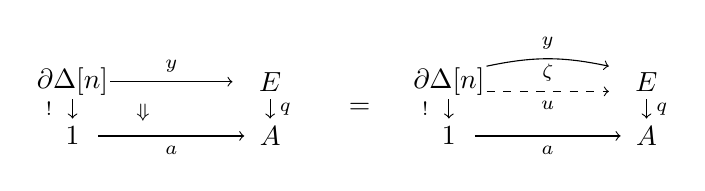
\begin{tikzpicture}[x=1.7em,y=1.4em]
  \node (a1) at (0,1.4) {$\partial\Delta[n]$};
  \node (b1) at (4.2,1.4) {$E$};
  \draw[->] (0.8,1.4) -- node[above]{$\scriptstyle y$} (3.4,1.4);
  \draw[->] (0,0.95) -- (0,0.45);
  \node at (-0.5,0.7) {$\scriptstyle !$};
  \node at (1.5,0.6) {$\scriptstyle\Downarrow\varkappa$};
  \draw[->] (4.2,0.95) -- node[right]{$\scriptstyle q$} (4.2,0.45);
  \node (c1) at (0,0) {$1$};
  \node (d1) at (4.2,0) {$A$};
  \draw[->] (0.55,0) -- node[below]{$\scriptstyle a$} (3.65,0);
  \node at (6.1,0.7) {$=$};
  \begin{scope}[shift={(8.0,0)}]
    \node (a2) at (0,1.4) {$\partial\Delta[n]$};
    \node (b2) at (4.2,1.4) {$E$};
    \draw[->] (0.8,1.8) to[bend left=12] node[above,pos=0.5]{$\scriptstyle y$} (3.4,1.8);
    \draw[->,dashed] (0.8,1.15) -- node[above,pos=0.5]{$\scriptstyle\zeta$}
      node[below,pos=0.5]{$\scriptstyle u$} (3.4,1.15);
    \draw[->] (0,0.95) -- (0,0.45);
    \node at (-0.5,0.7) {$\scriptstyle !$};
    \draw[->] (4.2,0.95) -- node[right]{$\scriptstyle q$} (4.2,0.45);
    \node (c2) at (0,0) {$1$};
    \node (d2) at (4.2,0) {$A$};
    \draw[->] (0.55,0) -- node[below]{$\scriptstyle a$} (3.65,0);
  \end{scope}
\end{tikzpicture}
\end{center}
由构造，右方所示 $q$-余笛卡尔提升的余定义域\trFunctor{}落入 $a$ 之上的纤维中。
现在，$\varkappa$ 在最终顶点 $\{n\}\colon 1\to\partial\Delta[n]$ 处的分量是
$\mathrm{id}_{a}$，故由第 5 章中的\cref{lem:isomorphism-stability}(ii)，表示
2-\trCell{} $\zeta\{n\}$ 的分量 $z\{n\}$ 是一个\trIsomorphism。特别地，
\trElement{} $u\{n\}\colon 1\to E$ \trIsomorphism{}于 $E_{a}$ 的\trTerminal{}%
元素 $y\{n\}=ta$，于是我们可以动用命题 F.1.1(vi) 的\trUniversalProperty{}把
$u$ 扩张成一个单纯形：
\begin{center}
\begin{tikzpicture}[x=1.8em,y=1.4em]
  \node (tl) at (0,1.4) {$\partial\Delta[n]$};
  \node (tr) at (4.8,1.4) {$E_{a}$};
  \draw[->] (tl) -- node[above]{$\scriptstyle u$} (tr);
  \draw[right hook->] (0,0.95) -- (0,0.45);
  \draw[->,dashed] (0.9,0.25) -- (4.0,1.15);
  \node at (2.7,0.95) {$\scriptstyle v$};
  \node (bl) at (0,0) {$\Delta[n]$};
\end{tikzpicture}
\end{center}
这份数据定义一个新的\trLifting{}问题
\begin{rveq}\label{eq:inductive-lifting-problem}
\begin{tikzpicture}[x=1.5em,y=1.5em]
  \node (tl) at (0,1.6) {$\partial\Delta[n]$};
  \node (tm) at (7.9,1.6) {$\partial\Delta[n]\times\Delta[1]\cup\Delta[n]\times\{1\}$};
  \node (tr) at (15.2,1.6) {$E$};
  \node (bl) at (0,0) {$\Delta[n]$};
  \node (bm) at (7.9,0) {$\Delta[n]\times\Delta[1]$};
  \node (br) at (15.2,0) {$A$};
  \draw[right hook->] (1.5,1.6) -- node[below]{$\scriptstyle i_{0}$} (4.3,1.6);
  \draw[->] (11.6,1.6) -- node[above]{$\scriptstyle z\cup v$} (14.0,1.6);
  \draw[right hook->] (1.2,0) -- node[below]{$\scriptstyle i_{0}$} (4.5,0);
  \draw[->] (11.4,0) -- node[above]{$\scriptstyle xk$} (14.0,0);
  \draw[right hook->] (0,1.1) -- (0,0.5);
  \draw[right hook->] (7.9,1.1) -- (7.9,0.5);
  \draw[->] (15.2,1.1) -- node[right]{$\scriptstyle q$} (15.2,0.5);
  \draw[->] (0.9,2.5) to[bend left=14] node[above]{$\scriptstyle y$} (14.3,2.5);
  \draw[->] (0.9,-0.9) to[bend right=14] node[below]{$\scriptstyle x$} (14.3,-0.9);
\end{tikzpicture}
\end{rveq}
我们按归纳法求解它：从含有 $\Delta[n]\times\{1\}$ 之面的那个
$(n+1)$-\trSimplex{}开始，为 $\Delta[n]\times\Delta[1]$ 中未出现于
$\partial\Delta[n]\times\Delta[1]\cup\Delta[n]\times\{1\}$ 的那 $n+1$ 个
$(n+1)$-\trSimplex{}逐一选取提升。除最后一个外，其余都可以借助对%
\trIsofibration{} $q$ 提升内\trHorn{}来实现。对于最后的

那个\trSimplex，我们必须求解一个外\trHorn{}\trLifting{}问题
\begin{center}
\begin{tikzpicture}[x=1.7em,y=1.4em]
  \node (d1) at (0,1.4) {$\Delta[1]$};
  \node (lh) at (5.0,1.4) {$\Lambda^{n+1}[n+1]$};
  \node (E)  at (9.8,1.4) {$E$};
  \draw[right hook->] (0.85,1.4) -- node[below]{$\scriptstyle\{n,n+1\}$} (3.3,1.4);
  \draw[->] (6.9,1.4) -- (8.5,1.4);
  \draw[->] (0.7,2.1) to[bend left=14] node[above,pos=0.5]{$\scriptstyle z\{n\}$} (9.1,2.1);
  \draw[right hook->] (5.0,0.95) -- (5.0,0.45);
  \draw[->] (9.8,0.95) -- node[right]{$\scriptstyle q$} (9.8,0.45);
  \node (dn) at (5.0,0) {$\Delta[n+1]$};
  \node (A)  at (9.8,0) {$A$};
  \draw[->] (dn) -- (A);
  \draw[->,dashed] (6.4,0.25) -- (9.2,1.15);
\end{tikzpicture}
\end{center}
但在此情形中，外\trHorn{}的最后一条边是\trIsomorphism{} $z\{n\}$，故第 1 章中的%
\cref{prop:special-outer-horn-lifting}也容许其求解。于是，提升
\eqref{eq:inductive-lifting-problem}限制而定义出原\trLifting{}问题所求的解，
这就证明了 $q\colon E\twoheadrightarrow A$ 容有一个\trRightAdjoint\trRightInverse。
\end{proof}

经由\cref{lem:opposite-qcat-biequivalence}的宇宙论\trBiequivalence{}
$(-)^{\mathrm{op}}\colon\QCat\simeq\QCat^{\mathrm{co}}$，
\cref{prop:cocartesian-rari-terminal-elements}之证明可以对偶化，以证明：诸%
\trQuasiCategory{}的一个\trCartesianFibration{}容有一个%
\trLeftAdjoint\trRightInverse，当且仅当每条纤维拥有一个\trInitial{}元素
（见\cref{ex:cartesian-lari-initial-elements}）。

\cref{prop:cocartesian-rari-terminal-elements}之证明颇倚重「解析的」技巧。
尽管如此，其结论可转移到任何\trBiequivalence{}于诸\trQuasiCategory{}的%
\trInfinityCosmos{}的\trInfinityCosmos。

\begin{proposition}\label{prop:pointwise-terminal-cocartesian-rari}
在一个 $(\infty,1)$-\trCategory{}的\trInfinityCosmos{}中，一个%
\trCocartesianFibration{} $q\colon E\twoheadrightarrow A$ 容有一个%
\trRightAdjoint\trRightInverse{} $t\colon A\to E$，当且仅当对每个\trElement{}
$a\colon 1\to A$，纤维 $E_{a}$ 拥有一个\trTerminal{}元素。
\end{proposition}

\begin{proof}
「带\trRightAdjoint\trRightInverse{}的\trIsofibration{}之诸纤维容有%
\trTerminal{}元素」这一方向的论证，与\cref{prop:cocartesian-rari-terminal-elements}
之证明中所给者相同。为证其逆，设 $q\colon E\twoheadrightarrow A$ 是一个
$(\infty,1)$-\trCategory{}的\trInfinityCosmos{} $\mathcal{K}$ 中的一个%
\trCocartesianFibration，带有如下性质：对底的每个\trElement{} $a\colon 1\to A$，
纤维 $E_{a}$ 拥有一个\trTerminal{}元素。由命题 10.2.1，我们可以动用底拟范畴%
\trBiequivalence{} $(-)_{0}\colon\mathcal{K}\Rightarrow\QCat$ 而断言：一旦证得
$q_{0}\colon E_{0}\to A_{0}$ 满足%
\cref{prop:cocartesian-rari-terminal-elements}的前提，$q$ 便容有一个%
\trRightAdjoint\trRightInverse。

宇宙论\trFunctor{}保持\trCocartesianFibration，故底映射
$q_{0}\colon E_{0}\to A_{0}$ 定义诸\trQuasiCategory{}的一个%
\trCocartesianFibration。由\cref{obs:elements-of-underlying-qcat}，底拟范畴
$A_{0}$ 的诸\trElement{}与∞-\trCategory{} $A$ 的诸\trElement{}双射地对应。由
假设，对每个\trElement{} $a\colon 1\to A$，∞-\trCategory{} $E_{a}$ 容有一个%
\trTerminal{}元素，故由命题 10.1.4，底拟范畴 $(E_{a})_{0}$ 亦然。如此我们看到：
诸\trQuasiCategory{}的\trCocartesianFibration{}
$q_{0}\colon E_{0}\to A_{0}$ 的每条纤维都容有一个\trTerminal{}%
元素。由\cref{prop:cocartesian-rari-terminal-elements}，$q_{0}$ 容有一个%
\trRightAdjoint\trRightInverse。如今由命题 10.3.6，我们可以断言
$q\colon E\twoheadrightarrow A$ 在 $\mathcal{K}$ 中容有一个%
\trRightAdjoint\trRightInverse，如所望。
\end{proof}

\cref{prop:pointwise-terminal-cocartesian-rari}的一个重要特例，证明了围绕
命题 4.1.6 的讨论中所许诺的一个结果：在一个 $(\infty,1)$-\trCategory{}的%
\trInfinityCosmos{}中，一个\trFunctor{} $f\colon B\to A$ 容有一个右伴随，恰当
对每个\trElement{} $a\colon 1\to A$，∞-\trCategory{}
$\mathrm{Hom}_{A}(f,a)$ 容有一个\trTerminal{}元素之时：即余单位分量
$\qcor{\varepsilon a}\colon 1\to\mathrm{Hom}_{A}(f,a)$。用 Mac Lane
[81, \S III.1] 的术语来说，这条\trUniversalProperty{}把 $\qcor{\varepsilon a}$
展示为从\trFunctor{} $f$ 到\trElement{} $a$ 的一支「泛箭头」。

\begin{corollary}\label{cor:right-adjoint-terminal-elements}
在一个 $(\infty,1)$-\trCategory{}的\trInfinityCosmos{}中，一个\trFunctor{}
$f\colon B\to A$ 容有一个右伴随，当且仅当对每个\trElement{} $a\colon 1\to A$，
\trCommaInfinityCategory{} $\mathrm{Hom}_{A}(f,a)$ 容有一个\trTerminal{}元素。
\end{corollary}

\begin{proof}
命题 4.1.6 表明：在任何\trInfinityCosmos{}中，$f\colon B\to A$ 容有一个右伴随，
当且仅当 $\mathrm{Hom}_{A}(f,A)$ 容有 $A$ 上的一个\trTerminal{}元素——意即
$p_{1}\colon\mathrm{Hom}_{A}(f,A)\twoheadrightarrow A$ 容有一个%
\trRightAdjoint\trRightInverse。由第 5 章中的\cref{cor:comma-domain-projections}，
这个\trFunctor{}是一个\trCocartesianFibration，故%
\cref{prop:pointwise-terminal-cocartesian-rari}告诉我们：$p_{1}$ 容有一个%
\trRightAdjoint\trRightInverse，当且仅当每条纤维 $\mathrm{Hom}_{A}(f,a)$
容有一个\trTerminal{}元素。
\end{proof}

\cref{prop:pointwise-terminal-cocartesian-rari}蕴含：$(\infty,1)$-%
\trCategory{}之间的诸\trModule{}容有一个类似的「逐点」可表示性条件，它刻画
那些在定义 7.4.7 的意义下被一个\trFunctor{}协变地或反变地表示的\trModule。

\begin{corollary}\label{cor:pointwise-covariant-representability}
在一个 $(\infty,1)$-\trCategory{}的\trInfinityCosmos{}中，一个\trModule{}
$A\xrightarrow{E}B$ 是协变表示的，当且仅当对每个\trElement{} $a\colon 1\to A$，
\trModule{} $1\xrightarrow{E(1,a)}B$ 是协变表示的；而后一情形成立，当且仅当每个
∞-\trCategory{} $E(1,a)$ 容有一个\trTerminal{}元素。
\end{corollary}

\begin{proof}
由第 8 章中的\cref{prop:detect-representable-modules}，由 $(q,p)\colon E\twoheadrightarrow A\times B$ 所编码的%
\trModule{} $A\xrightarrow{E}B$ 是协变表示的，当且仅当其左腿
$q\colon E\twoheadrightarrow A$ 容有一个\trRightAdjoint\trRightInverse{}
$r\colon A\to E$，此时 $E\cong\mathrm{Hom}_{B}(B,pr)$。由引理 7.4.3，左腿
$q\colon E\twoheadrightarrow A$ 定义一个\trCocartesianFibration，故由%
\cref{prop:pointwise-terminal-cocartesian-rari}，$q$ 容有一个%
\trRightAdjoint\trRightInverse，当且仅当在每个\trElement{} $a\colon 1\to A$
之上的纤维 $E_{a}$ 容有一个\trTerminal{}元素。对每个\trElement{}
$a\colon 1\to A$，\trModule{} $1\xrightarrow{E(1,a)}B$ 由沿
$a\times\mathrm{id}\colon 1\times B\to A\times B$ 取\trPullback{}而给出，从而%
\trIsomorphism{}于\trModule{} $1\xrightarrow{E_{a}}B$。再次应用第 8 章中的%
\cref{prop:detect-representable-modules}：
这个\trModule{}被某个\trElement{}协变表示，当且仅当 $!\colon E_{a}\to 1$
容有一个\trRightAdjoint\trRightInverse，而后一情形成立，当且仅当∞-%
\trCategory{} $E_{a}\cong E(1,a)$ 容有一个\trTerminal{}元素。
\end{proof}

我们的下一条结果关乎绝对提升图——定义 2.3.8 用它们来定义一个图表族的%
\trLimit{}或\trColimit。就陈述诸如命题 2.3.15 之类的结果而言，考虑诸图表的族
而非单个图表，自有其一番雅致；但逐一地确立\trLimit{}与\trColimit{}的存在性
——每次一个图表——同样有用。在 $(\infty,1)$-\trCategory{}的诸%
\trInfinityCosmos{}中，这类约化是可能的，其凭据如下：

\begin{proposition}\label{prop:absolute-right-lifting-pointwise}
在一个 $(\infty,1)$-\trCategory{}的\trInfinityCosmos{}中：
\begin{enumerate}[label=(\roman*)]
\item 一个\trFunctor{} $g\colon C\to A$ 穿过一个\trFunctor{} $f\colon B\to A$
  容有一个\trAbsoluteRightLifting，当且仅当对一切\trElement{} $c\colon 1\to C$，%
  \trCommaInfinityCategory{} $\mathrm{Hom}_{A}(f,gc)$ 容有一个\trTerminal{}元素。
\item 如左下方的三角形
\begin{center}
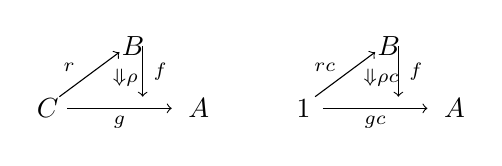
\begin{tikzpicture}[x=1.4em,y=1.4em]
  \node (b) at (2.2,1.6) {$B$};
  \node (c) at (0,0) {$C$};
  \node (a) at (3.9,0) {$A$};
  \draw[->] (0.3,0.3) -- (1.85,1.45);
  \node at (0.55,1.05) {$\scriptstyle r$};
  \node at (2.0,0.78) {$\scriptstyle\Downarrow\rho$};
  \draw[->] (2.45,1.6) -- (2.45,0.3);
  \node at (2.9,0.95) {$\scriptstyle f$};
  \draw[->] (0.5,0) -- (3.2,0);
  \node at (1.85,-0.36) {$\scriptstyle g$};
  \begin{scope}[shift={(6.6,0)}]
    \node (b2) at (2.2,1.6) {$B$};
    \node (c2) at (0,0) {$1$};
    \node (a2) at (3.9,0) {$A$};
    \draw[->] (0.3,0.3) -- (1.85,1.45);
    \node at (0.55,1.05) {$\scriptstyle rc$};
    \node at (2.0,0.78) {$\scriptstyle\Downarrow\rho c$};
    \draw[->] (2.45,1.6) -- (2.45,0.3);
    \node at (2.9,0.95) {$\scriptstyle f$};
    \draw[->] (0.5,0) -- (3.2,0);
    \node at (1.85,-0.36) {$\scriptstyle gc$};
  \end{scope}
\end{tikzpicture}
\end{center}
  显示 $r$ 为 $g$ 穿过 $f$ 的一个\trAbsoluteRightLifting，当且仅当对一切\trElement{}
  $c\colon 1\to C$，如右上方的受限三角形显示 $rc$ 为 $gc$ 穿过 $f$ 的一个%
  \trAbsoluteRightLifting。
\item 一个\trFunctor{} $g\colon C\to A$ 穿过一个\trFunctor{} $f\colon B\to A$
  容有一个\trAbsoluteRightLifting，当且仅当对一切\trElement{} $c\colon 1\to C$，$gc$ 穿过
  $f$ 都存在一个如下左方所示的\trAbsoluteRightLifting
\begin{center}
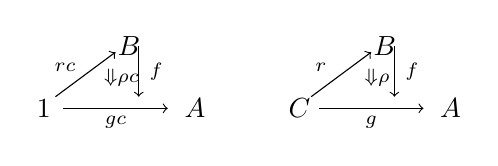
\begin{tikzpicture}[x=1.4em,y=1.4em]
  \node (b) at (2.2,1.6) {$B$};
  \node (c) at (0,0) {$1$};
  \node (a) at (3.9,0) {$A$};
  \draw[->] (0.3,0.3) -- (1.85,1.45);
  \node at (0.55,1.05) {$\scriptstyle rc$};
  \node at (2.0,0.78) {$\scriptstyle\Downarrow\rho c$};
  \draw[->] (2.45,1.6) -- (2.45,0.3);
  \node at (2.9,0.95) {$\scriptstyle f$};
  \draw[->] (0.5,0) -- (3.2,0);
  \node at (1.85,-0.36) {$\scriptstyle gc$};
  \begin{scope}[shift={(6.6,0)}]
    \node (b2) at (2.2,1.6) {$B$};
    \node (c2) at (0,0) {$C$};
    \node (a2) at (3.9,0) {$A$};
    \draw[->] (0.3,0.3) -- (1.85,1.45);
    \node at (0.55,1.05) {$\scriptstyle r$};
    \node at (2.0,0.78) {$\scriptstyle\Downarrow\rho$};
    \draw[->] (2.45,1.6) -- (2.45,0.3);
    \node at (2.9,0.95) {$\scriptstyle f$};
    \draw[->] (0.5,0) -- (3.2,0);
    \node at (1.85,-0.36) {$\scriptstyle g$};
  \end{scope}
\end{tikzpicture}
\end{center}
  在此情形，如右上方 $g$ 穿过 $f$ 的\trAbsoluteRightLifting{}的诸分量\trIsomorphism{}于相应的
  逐点绝对提升：$r_{c}\cong rc$ 且 $\rho_{c}\cong\rho c$。
\end{enumerate}
\end{proposition}

\begin{proof}
第 3 章中的\cref{thm:trio-bijection}与\cref{thm:right-representability}表明：在任何\trInfinityCosmos{}中，一个\trFunctor{}
$g\colon C\to A$ 穿过 $f\colon B\to A$ 容有一个右提升，当且仅当余定义域投影%
\trFunctor{} $p_{1}\colon\mathrm{Hom}_{A}(f,g)\twoheadrightarrow C$ 容有一个%
\trRightAdjoint\trRightInverse。由第 5 章中的\cref{cor:comma-domain-projections}，
这个\trFunctor{}是一个\trCocartesianFibration。%
\cref{prop:pointwise-terminal-cocartesian-rari}证明：
在一个 $(\infty,1)$-\trCategory{}的\trInfinityCosmos{}中，
$p_{1}\colon\mathrm{Hom}_{A}(f,g)\twoheadrightarrow C$ 容有一个%
\trRightAdjoint\trRightInverse，当且仅当在\trElement{} $c\colon 1\to C$ 之上
的每条纤维 $\mathrm{Hom}_{A}(f,gc)$ 容有一个\trTerminal{}元素。这就证明了
第一款。

由于绝对提升图在限制下稳定，任何如左上方所示的\trAbsoluteRightLifting{}图表都限制而定义一个
逐点的\trAbsoluteRightLifting{}图表，如右上方所示。为证其逆，设 $(rc,\rho c)$ 对任意%
\trElement{} $c\colon 1\to C$ 都定义 $gc$ 穿过 $f$ 的一个\trAbsoluteRightLifting。由第 3 章中的%
\cref{thm:right-representability}，由此可知每个\trCommaInfinityCategory{} $\mathrm{Hom}_{A}(f,gc)$ 都
拥有一个\trTerminal{}元素，于是由 (i)，$g\colon C\to A$ 必定容有穿过
$f\colon B\to A$ 的一个\trAbsoluteRightLifting{} $(s,\sigma)$。据其\trUniversalProperty，对
$(r,\rho)$ 经由一支 2-\trCell{} $\tau\colon r\Rightarrow s$ 穿过 $(s,\sigma)$
作分解，使得 $\rho=\sigma\cdot f\tau$。由于 $(rc,\rho c)$ 与 $(sc,\sigma c)$
都是\trAbsoluteRightLifting{}图表，我们知道每个分量 $\tau c$ 都是\trIsomorphism。从而，由%
\cref{lem:pointwise-natural-isomorphism}，$\tau$ 是一个\trIsomorphism，于是
$(r,\rho)$ 也是一个\trAbsoluteRightLifting{}图表，如所望。

第三款是对前两款的一个便利总结。若 $gc$ 穿过 $f$ 容有一个\trAbsoluteRightLifting，则
$\mathrm{Hom}_{A}(f,gc)$ 拥有一个\trTerminal{}元素，而 (i) 保证 $g$ 穿过 $f$
的某个\trAbsoluteRightLifting{}存在。$(r,\rho)$ 在 $c$ 处的分量定义 $gc$ 穿过 $f$ 的第二个%
\trAbsoluteRightLifting，从而诱导出所宣称的那些\trIsomorphism。
\end{proof}

作为一条推论，我们可以证成注 2.3.9 中所作的断言。

\begin{corollary}\label{cor:pointwise-limits-adjoint}
在一个 $(\infty,1)$-\trCategory{}的\trInfinityCosmos{}中，若 $A$ 是一个对形状
$J$ 的每个图表 $d\colon 1\to A^{J}$ 都容有\trLimit{}的∞-\trCategory，则 $A$
容有形状 $J$ 的一切\trLimit：也就是说，常值图表\trFunctor{}容有一个右伴随
\begin{center}
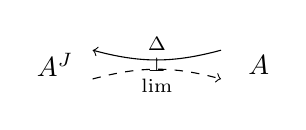
\begin{tikzpicture}[x=1.6em,y=1.3em]
  \node (AJ) at (0,0) {$A^{J}$};
  \node (A)  at (4.6,0) {$A$};
  \draw[->] (3.75,0.4) to[bend left=15] node[above]{$\scriptstyle\Delta$} (0.85,0.4);
  \node at (2.3,0) {$\scriptstyle\perp$};
  \draw[->,dashed] (0.85,-0.4) to[bend left=15] node[below]{$\scriptstyle\lim$} (3.75,-0.4);
\end{tikzpicture}
\end{center}
\end{corollary}

\begin{proof}
由\cref{prop:absolute-right-lifting-pointwise}(iii)，\trFunctor{}
$\mathrm{id}\colon A^{J}\to A^{J}$ 穿过 $\Delta\colon A\to A^{J}$ 容有一个%
\trAbsoluteRightLifting，当且仅当每个图表 $d\colon 1\to A^{J}$ 穿过 $\Delta\colon A\to A^{J}$
都容有一个\trAbsoluteRightLifting。由定义 2.3.8，后一条件编码了「$A$ 容有图表 $d$ 的一个%
\trLimit」之所指；而由引理 2.3.7，前一条件编码了「$\Delta\colon A\to A^{J}$
容有一个右伴随」之所指。
\end{proof}

\cref{prop:absolute-right-lifting-pointwise}(ii) 的另一个证明是可能的。由第 3 章中的%
\cref{thm:trio-bijection}，一支 2-\trCell{} $\rho\colon fr\Rightarrow g$ 定义一个\trAbsoluteRightLifting，当且
仅当诱导\trFunctor{}
$\qcor{\rho}\colon\mathrm{Hom}_{B}(B,r)\to\mathrm{Hom}_{A}(f,g)$ 是居于
$C\times B$ 之上的一个\trFiberedEquivalence。正如我们现在将要发现的，在
$(\infty,1)$-\trCategory{}的诸\trInfinityCosmos{}中，诸余/笛卡尔纤维化之间或
诸\trModule{}之间的\trEquivalence{}可以逐纤维地检测。正如构造余笛卡尔纤维化的%
\trRightAdjoint\trRightInverse{}时的策略一样，我们首先借助解析技巧对诸%
\trQuasiCategory{}证明这一结果。另类的解析证明可见于文献 [78, 3.3.1.5] 与
[5, 2.9]。随后我们动用\trModelIndependence{}断言：同样的结果在任意的
$(\infty,1)$-\trCategory{}的诸\trInfinityCosmos{}中成立。

\begin{proposition}\label{prop:fiberwise-equivalence-cartesian-functor}
诸\trQuasiCategory{}的\trCocartesianFibration{}之间的一个\trCartesianFunctor
\begin{center}
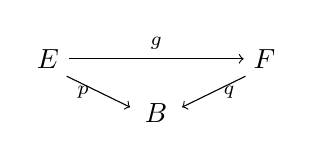
\begin{tikzpicture}[x=1.7em,y=1.4em]
  \node (E) at (0,1.4) {$E$};
  \node (F) at (4.6,1.4) {$F$};
  \node (B) at (2.3,0) {$B$};
  \draw[->] (E) -- node[above]{$\scriptstyle g$} (F);
  \draw[->] (0.4,0.95) -- node[left,pos=0.5]{$\scriptstyle p$} (1.75,0.15);
  \draw[->] (4.2,0.95) -- node[right,pos=0.5]{$\scriptstyle q$} (2.85,0.15);
\end{tikzpicture}
\end{center}
是一个\trFiberedEquivalence，当且仅当它是一个逐纤维等价，意即对每个\trElement{}
$b\colon 1\to B$，诱导的纤维间\trFunctor{} $g_{b}\colon E_{b}\to F_{b}$ 是一个%
\trEquivalence。
\end{proposition}

注意「纤维化等价」——$B$ 之上的\trEquivalence——与「逐纤维等价」——在 $B$
的诸\trElement{}之上的诸纤维上诱导\trEquivalence{}的映射——这两个术语之间的
微妙差别。本结果与紧随其后的\cref{prop:fiberwise-equivalence-cosmos}一道
表明：事实上，在
$(\infty,1)$-\trCategory{}的诸\trInfinityCosmos{}中，这两个概念对%
\trCartesianFunctor{}而言重合。

\begin{proof}
\trFiberedEquivalence{}在到纤维的拉回下稳定，故实质内容在于逆蕴含：任何在%
\trCocartesianFibration{}之间诱导逐纤维等价的\trCartesianFunctor{}都必然是一
个\trEquivalence。

这个\trCartesianFunctor{} $g$ 可以在切片 $\QCat_{/B}$ 中分解为一个%
\trEquivalence{}后接一个\trIsofibration。由第 5 章中的%
\cref{cor:equivalence-invariance}，该分解的中间对象仍是一个%
\trCocartesianFibration，而从这个中间对象出发、指向 $q\colon F\twoheadrightarrow B$
的\trIsofibration{}仍是一个\trCartesianFunctor。用与之\trEquivalence{}的%
\trCocartesianFibration{}替换 $p\colon E\twoheadrightarrow B$ 之后，因此只需
假设 $g\colon E\twoheadrightarrow F$ 既是一个\trIsofibration{}又是一个%
\trCartesianFunctor，\footnote{原书此处印作「$g\colon E\twoheadrightarrow B$」；
按上下文 $g$ 之余定义域为 $F$（见本条首图），疑为「$E\twoheadrightarrow F$」
之误，此处径改。——译者注}并设定每个诱导映射
$g_{b}\colon E_{b}\twoheadrightarrow F_{b}$ 都是一个\trTrivialFibration。在
这些假设下，我们必须证明 $g$ 自身是一个\trTrivialFibration。

为此，设给定一个\trLifting{}问题
\begin{center}
\begin{tikzpicture}[x=1.8em,y=1.4em]
  \node (tl) at (0,1.4) {$\partial\Delta[n]$};
  \node (tr) at (4.6,1.4) {$E$};
  \node (bl) at (0,0) {$\Delta[n]$};
  \node (br) at (4.6,0) {$F$};
  \draw[->] (tl) -- node[above]{$\scriptstyle e$} (tr);
  \draw[right hook->] (0,0.95) -- (0,0.45);
  \draw[->] (tr) -- node[right]{$\scriptstyle g$} (br);
  \draw[->] (bl) -- node[below]{$\scriptstyle f$} (br);
\end{tikzpicture}
\end{center}
于 $b\colon\Delta[n]\to B$ 之上。考虑收缩图表
\begin{center}
\begin{tikzpicture}[x=1.6em,y=1.3em]
  \node (a) at (0,1.6) {$\Delta[n]$};
  \node (b) at (6.2,1.6) {$\Delta[n]\times\Delta[1]$};
  \node (c) at (13.0,1.6) {$\Delta[n]$};
  \draw[->] (1.1,1.6) -- node[above]{$\scriptstyle\mathrm{id}\times\{0\}$} (3.4,1.6);
  \draw[->] (9.0,1.6) -- node[above]{$\scriptstyle r$} (11.3,1.6);
  \node at (1.0,0.55) {$\scriptstyle i\longmapsto(i,0)$};
  \node at (7.6,0.35) {$\scriptstyle(i,j)\longmapsto$};
  \node at (10.6,0.6) {$\scriptstyle\left\{\begin{array}{ll}i & \text{若 } j=0\\ n & \text{若 } j=1\end{array}\right.$};
\end{tikzpicture}
\end{center}

并选取一个逐点的 $p$-余笛卡尔提升
\begin{center}
\begin{tikzpicture}[x=1.9em,y=1.4em]
  \node (tl) at (0,1.4) {$\partial\Delta[n]\times\{0\}$};
  \node (tr) at (6.6,1.4) {$E$};
  \node (bl) at (0,0) {$\partial\Delta[n]\times\Delta[1]$};
  \node (br) at (6.6,0) {$B$};
  \draw[->] (tl) -- node[above]{$\scriptstyle e$} (tr);
  \draw[right hook->] (0,0.95) -- (0,0.45);
  \draw[->,dashed] (2.1,0.25) -- (5.8,1.15);
  \node at (3.5,0.95) {$\scriptstyle\chi$};
  \draw[->] (tr) -- node[right]{$\scriptstyle p$} (br);
  \draw[->] (bl) -- node[below]{$\scriptstyle br$} (br);
\end{tikzpicture}
\end{center}
如引理 F.4.8 所容许者。施加 $g$，我们得到一个空心柱面
\[
\partial\Delta[n]\times\Delta[1]\xrightarrow{\;\chi\;}E\xrightarrow{\;g\;}F
\]
由于 $g$ 是一个\trCartesianFunctor{}而 $\chi$ 是逐点 $p$-余笛卡尔的，故 $g\chi$
是逐点 $q$-余笛卡尔的。现在，由构造，单纯形
$f\colon\Delta[n]\times\{0\}\to F$ 在二者均有定义的子集
$\partial\Delta[n]\times\{0\}$ 上与 $g\chi\colon\Delta[n]\times\Delta[1]\to F$
相合。从而二者在其定义域之并上拼合成一个良定的单纯映射，于是为我们提供了第二
个\trLifting{}问题：
\begin{center}
\begin{tikzpicture}[x=1.9em,y=1.4em]
  \node (tl) at (0,1.4) {$\Delta[n]\times\{0\}\cup\Delta[n]\times\Delta[1]$};
  \node (tr) at (8.6,1.4) {$F$};
  \node (bl) at (0,0) {$\Delta[n]\times\Delta[1]$};
  \node (br) at (8.6,0) {$B$};
  \draw[->] (tl) -- node[above]{$\scriptstyle f\cup g\chi$} (tr);
  \draw[right hook->] (0,0.95) -- (0,0.45);
  \draw[->,dashed] (2.6,0.25) -- (7.8,1.15);
  \node at (4.4,0.95) {$\scriptstyle\rho$};
  \draw[->] (tr) -- node[right]{$\scriptstyle q$} (br);
  \draw[->] (bl) -- node[below]{$\scriptstyle br$} (br);
\end{tikzpicture}
\end{center}
它可以再度求解——由引理 F.4.8——给出一个逐点的 $q$-余笛卡尔提升 $\rho$。现在
注意：收缩 $r\colon\Delta[n]\times\Delta[1]\to\Delta[n]$ 被构造成把子集
$\Delta[n]\times\{1\}$ 映到顶点 $\{n\}$ 上，由此可知，$n$-\trSimplex
\[
\Delta[n]\times\{1\}\hookrightarrow\Delta[n]\times\Delta[1]\xrightarrow{\;br\;}B
\]
是最终顶点 $b_{n}\coloneqq b\cdot\{n\}$ 的一个退化像。现在观察到：柱面 $\chi$
与 $\rho$ 被定义为居于 $br\colon\Delta[n]\times\Delta[1]\to B$ 之上，故受限
映射
\[
\begin{gathered}
\partial\Delta[n]\times\{1\}\hookrightarrow\Delta[n]\times\Delta[1]
  \xrightarrow{\;\chi\;}E\\
\Delta[n]\times\{1\}\hookrightarrow\Delta[n]\times\Delta[1]
  \xrightarrow{\;\rho\;}F
\end{gathered}
\]
分别落入 $p$ 与 $q$ 的纤维 $E_{b_{n}}$ 与 $F_{b_{n}}$ 之中。于是，$\chi$ 与
$\rho$ 定义一个\trLifting{}问题
\begin{center}
\begin{tikzpicture}[x=1.8em,y=1.4em]
  \node (tl) at (0,1.4) {$\partial\Delta[n]$};
  \node (tr) at (5.0,1.4) {$E_{b_{n}}$};
  \node (bl) at (0,0) {$\Delta[n]$};
  \node (br) at (5.0,0) {$F_{b_{n}}$};
  \draw[->] (tl) -- node[above]{$\scriptstyle\chi\vert_{\{1\}}$} (tr);
  \draw[right hook->] (0,0.95) -- (0,0.45);
  \draw[->,dashed] (0.9,0.25) -- (4.2,1.15);
  \node at (2.3,0.95) {$\scriptstyle\gamma$};
  \draw[double,->] (tr) -- node[right]{$\scriptstyle g_{b_{n}}$} (br);
  \draw[->] (bl) -- node[below]{$\scriptstyle\rho\vert_{\{1\}}$} (br);
\end{tikzpicture}
\end{center}

它可以求解，因为右侧的纤维间映射按假设是一个\trTrivialFibration。现在，左上
三角形告诉我们：$\chi$ 与 $\gamma$ 在二者均有定义的子集
$\partial\Delta[n]\times\{1\}$ 上相合。于是，这些映射拼合而给出定义域之并上
的一个良定的单纯映射——即下方图表右侧那个\trLifting{}问题中画为上横边的
那个映射：
\begin{center}
\begin{tikzpicture}[x=1.8em,y=1.5em]
  \node (a) at (0,1.6) {$\partial\Delta[n]\times\{0\}$};
  \node (b) at (7.4,1.6) {$\Delta[n]\times\{1\}\cup\partial\Delta[n]\times\Delta[1]$};
  \node (c) at (15.0,1.6) {$E$};
  \node (d) at (0,0) {$\Delta[n]\times\{0\}$};
  \node (e) at (7.4,0) {$\Delta[n]\times\Delta[1]$};
  \node (f) at (15.0,0) {$F$};
  \draw[right hook->] (2.4,1.6) -- (4.7,1.6);
  \draw[->] (10.4,1.6) -- node[above]{$\scriptstyle g\chi$} (13.2,1.6);
  \draw[right hook->] (0,1.15) -- (0,0.45);
  \draw[right hook->] (7.4,1.15) -- (7.4,0.45);
  \draw[right hook->] (2.2,0) -- (4.6,0);
  \draw[->] (10.2,0) -- node[above]{$\scriptstyle\rho$} (13.2,0);
  \draw[->] (c) -- node[right]{$\scriptstyle g$} (f);
  \draw[->,dashed] (8.4,0.5) -- (14.0,1.3);
  \draw[->] (1.0,2.7) to[bend left=12] node[above]{$\scriptstyle e$} (14.2,2.7);
  \draw[->] (1.0,-1.1) to[bend right=12] node[below]{$\scriptstyle f$} (14.2,-1.1);
\end{tikzpicture}
\end{center}
一个标准论证表明：右侧方块中的\trLifting{}问题，可以通过填充一列内\trHorn{}与
一支形状为 $\Lambda^{n+1}[n+1]$ 的单独外\trHorn{}而求解——后者的最后一条边是
在 $b_{n}$ 处的退化单纯形的一个余笛卡尔提升。第 5 章中的%
\cref{lem:isomorphism-stability}观察到：退化单纯形的余笛卡尔提升都是%
\trIsomorphism，故这最后一支\trHorn{}实际上是一支「特殊外\trHorn」——其第一
条边可逆。从而，由定理 D.5.1，它可以对\trIsofibration{} $p$ 提升之。这一构造
填充了空心柱面定义域端的\trSphere，求解了原来的\trLifting{}问题。
\end{proof}

\begin{proposition}[余笛卡尔纤维化的逐纤维等价]\label{prop:fiberwise-equivalence-cosmos}
在一个 $(\infty,1)$-\trCategory{}的\trInfinityCosmos{}中，%
\trCocartesianFibration\footnote{原书环境头括注印作「笛卡尔纤维化的逐纤维
等价」（fiberwise equivalences of cartesian fibrations），与本条陈述及证明
所论之余笛卡尔纤维化（同命题 12.2.11）相抵，疑为原书将 cocartesian 误作
cartesian 之误，此处径改。——译者注}之间的一个\trCartesianFunctor
\begin{center}
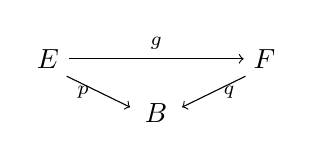
\begin{tikzpicture}[x=1.7em,y=1.4em]
  \node (E) at (0,1.4) {$E$};
  \node (F) at (4.6,1.4) {$F$};
  \node (B) at (2.3,0) {$B$};
  \draw[->] (E) -- node[above]{$\scriptstyle g$} (F);
  \draw[->] (0.4,0.95) -- node[left,pos=0.5]{$\scriptstyle p$} (1.75,0.15);
  \draw[->] (4.2,0.95) -- node[right,pos=0.5]{$\scriptstyle q$} (2.85,0.15);
\end{tikzpicture}
\end{center}
是一个\trFiberedEquivalence，当且仅当它是一个逐纤维等价，意即对每个\trElement{}
$b\colon 1\to B$，诱导的纤维间\trFunctor{} $g_{b}\colon E_{b}\to F_{b}$ 是一个%
\trEquivalence。
\end{proposition}

\begin{proof}
\trCocartesianFibration{}之间的一个\trEquivalence{}必然是逐纤维等价，故只需
证明其逆。由命题 10.2.2 与命题 10.2.1，若 $\mathcal{K}$ 是一个
$(\infty,1)$-\trCategory{}的\trInfinityCosmos{}而 $B$ 是 $\mathcal{K}$ 中的
一个∞-\trCategory，则底拟范畴\trFunctor{}诱导一个宇宙论\trBiequivalence{}
$(-)_{0}\colon\mathcal{K}_{/B}\Rightarrow\QCat_{/B_{0}}$。由推论 10.3.2，
这个宇宙论\trBiequivalence{}反射\trEquivalence；而由命题 10.1.4，
$(-)_{0}\colon\mathcal{K}\to\QCat$ 保持\trCocartesianFibration{}及其间的%
\trCartesianFunctor。于是，为证一个既是\trCartesianFunctor{}又是逐纤维等价的
$g\colon E\to F$ 是 $B$ 之上的一个\trEquivalence
$B_{0}$ 之上的一个\trEquivalence，为此我们验证：这个\trFunctor{}满足%
\cref{prop:fiberwise-equivalence-cartesian-functor}的前提。由%
\cref{obs:elements-of-underlying-qcat}，底拟范畴 $B_{0}$ 的诸\trElement{}与
∞-\trCategory{} $B$ 的诸\trElement{}双射地对应，而宇宙论\trFunctor{}
$(-)_{0}\colon\mathcal{K}\to\QCat$ 既保持诸纤维又保持诸\trEquivalence。如此
我们看到：$g_{0}\colon E_{0}\to F_{0}$ 对一切 $b\colon 1\to B_{0}$ 都是逐纤维
等价。由\cref{prop:fiberwise-equivalence-cartesian-functor}，这个\trFunctor{}%
定义一个\trFiberedEquivalence，从而 $g$ 亦然。
\end{proof}

\begin{corollary}\label{cor:discrete-cartesian-trivial-contractible}
在一个 $(\infty,1)$-\trCategory{}的\trInfinityCosmos{}中，一个离散%
\trCartesianFibration{}是一个\trTrivialFibration，当且仅当它的诸纤维是%
\trContractible。
\end{corollary}

\begin{proof}
若 $p\colon E\twoheadrightarrow B$ 是一个离散\trCartesianFibration，则 $p$
定义一个\trCartesianFunctor
\begin{center}
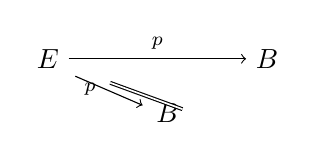
\begin{tikzpicture}[x=1.8em,y=1.4em]
  \node (E)  at (0,1.4) {$E$};
  \node (Bt) at (4.4,1.4) {$B$};
  \node (Bb) at (2.4,0) {$B$};
  \draw[->] (E) -- node[above]{$\scriptstyle p$} (Bt);
  \draw[->] (0.55,0.95) -- node[left,pos=0.45]{$\scriptstyle p$} (1.9,0.2);
  \draw[double] (1.25,0.78) -- (2.7,0.1);
\end{tikzpicture}
\end{center}
其余定义域是恒同的离散\trCartesianFibration。结论现在作为%
\cref{prop:fiberwise-equivalence-cosmos}之结果的一个特例而出现。
\end{proof}

\cref{prop:fiberwise-equivalence-cosmos}的结果可以延拓到诸\trModule{}：

\begin{corollary}[模的等价由逐纤维确定]\label{cor:module-equivalence-fiberwise}
在一个 $(\infty,1)$-\trCategory{}的\trInfinityCosmos{}中，从 $A$ 到 $B$ 的诸%
\trModule{} $E$ 与 $F$ 之间的一个映射
\begin{center}
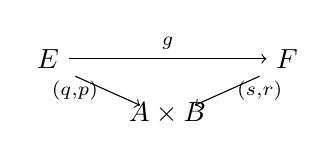
\begin{tikzpicture}[x=1.8em,y=1.4em]
  \node (E)  at (0,1.4) {$E$};
  \node (F)  at (4.8,1.4) {$F$};
  \node (AB) at (2.4,0) {$A\times B$};
  \draw[->] (E) -- node[above]{$\scriptstyle g$} (F);
  \draw[->] (0.55,0.95) -- node[left,pos=0.5]{$\scriptstyle(q,p)$} (1.85,0.2);
  \draw[->] (4.25,0.95) -- node[right,pos=0.5]{$\scriptstyle(s,r)$} (2.95,0.2);
\end{tikzpicture}
\end{center}
是一个\trEquivalence，当且仅当它是一个逐纤维等价，意即对每个\trElement{}
$a\colon 1\to A$ 与 $b\colon 1\to B$，诱导的纤维间\trFunctor{}
$g_{a,b}\colon E(b,a)\to F(b,a)$ 是一个\trEquivalence。
\end{corollary}

\begin{proof}
由引理 7.4.3 回忆起：左腿 $q\colon E\twoheadrightarrow A$ 与
$s\colon F\twoheadrightarrow A$ 是\trCocartesianFibration，而\trFunctor{} $g$
在它们之间定义一个\trCartesianFunctor。从而，由%
\cref{prop:fiberwise-equivalence-cosmos}，$g$ 是一个\trEquivalence，当且仅当对
每个\trElement{} $a\colon 1\to A$，拉回 $g_{a}\colon E(1,a)\to F(1,a)$ 是一个%
\trEquivalence。这些∞-\trCategory{}中的每一个都定义一个从 $1$ 到 $B$ 的%
\trModule，故再次由引理 7.4.3，拉回后的投影 $p\colon E(1,a)\twoheadrightarrow B$
与 $r\colon F(1,a)\twoheadrightarrow B$ 是\trCartesianFibration{}，而 $g_{a}$
在它们之间定义一个\trCartesianFunctor。由\cref{prop:fiberwise-equivalence-cosmos}
的对偶，这个\trFunctor{}是一个\trEquivalence，当且仅当对每个\trElement{}
$b\colon 1\to B$，纤维上的诱导作用
$g_{a,b}\colon E(b,a)\to F(b,a)$\footnote{原书此处印作
「$g_{a,b}\colon E(b,a)\to F(a,b)$」；按本条陈述（其纤维间\trFunctor{}作
$g_{a,b}\colon E(b,a)\to F(b,a)$）疑为 $F(b,a)$ 之误，此处径改。——译者注}
是一个\trEquivalence。这就证明了所述结果。
\end{proof}

这一结果的一个原型性特例，刻画了 $(\infty,1)$-\trCategory{}之间的诸%
\trAdjunction{}的单位或余单位：

\begin{corollary}\label{cor:counit-mapping-equivalences}
在一个 $(\infty,1)$-\trCategory{}的\trInfinityCosmos{}中，一支 2-\trCell{}
$\varepsilon\colon fu\Rightarrow\mathrm{id}_{A}$ 定义伴随 $f\dashv u$ 的余单位，
当且仅当诱导\trFunctor{}
$\qcor{\varepsilon\cdot f(-)}\colon\mathrm{Hom}_{B}(B,u)\to\mathrm{Hom}_{A}(f,A)$
——居于 $A\times B$ 之上——对每个\trElement{} $a\colon 1\to A$ 与
$b\colon 1\to B$ 都定义诸\trMappingSpace{}的等价
$\mathrm{Hom}_{B}(b,ua)\simeq\mathrm{Hom}_{A}(fb,a)$。
\end{corollary}

\cref{cor:module-equivalence-fiberwise}也可以应用于刻画诸 $(\infty,1)$-%
\trCategory{}之间的\trFullyFaithful{}\trFunctor{}与等价。

\begin{proposition}\label{prop:fully-faithful-pointwise}
在一个 $(\infty,1)$-\trCategory{}的\trInfinityCosmos{}中，一个\trFunctor{}
$f\colon A\to B$ 是\trFullyFaithful，当且仅当对一切\trElement{}
$a,a'\colon 1\to A$，其在诸\trMappingSpace{}上的作用
$f_{a,a'}\colon\mathrm{Hom}_{A}(a,a')\to\mathrm{Hom}_{B}(fa,fa')$ 定义诸%
\trDiscrete{}∞-\trCategory{}的一个等价。
\end{proposition}

\begin{proof}
第 3 章中的\cref{cor:fully-faithful}把一个\trFunctor{} $f\colon A\to B$ 定义为%
\trFullyFaithful，当且仅当诱导\trFunctor{}
$A^{2}\to\mathrm{Hom}_{B}(f,f)$——介于从 $A$ 到 $A$ 的诸\trModule{}之间——是
一个\trEquivalence。由\cref{cor:module-equivalence-fiberwise}，这成立当且仅当
这个映射定义一个逐纤维等价，而这恰好意味着：对一切\trElement{}
$a,a'\colon 1\to A$，其在诸\trMappingSpace{}上的作用
$f_{a,a'}\colon\mathrm{Hom}_{A}(a,a')\to\mathrm{Hom}_{B}(fa,fa')$ 定义诸%
\trDiscrete{}∞-\trCategory{}的一个等价。
\end{proof}

我们现在表明：$(\infty,1)$-\trCategory{}的等价恰好是那些在一个合适意义下逐点%
\trFullyFaithful{}且\trEssentiallySurjective\trFunctor。在文献 [102] 中，
Rezk 称这一结果为「拟范畴理论的基本定理」。我们的证明把综合技巧与解析技巧
混合起来：

\begin{theorem}[$(\infty,1)$-范畴理论的基本定理]\label{thm:fundamental-theorem}
在一个 $(\infty,1)$-\trCategory{}的\trInfinityCosmos{}中，一个\trFunctor{}
$f\colon A\to B$ 是一个\trEquivalence，当且仅当它
\begin{enumerate}[label=(\roman*)]
\item 是\textbf{\trFullyFaithful}：意即对一切\trElement{} $a,a'\colon 1\to A$，
  诱导映射
\[
\mathrm{Hom}_{A}(a,a')\longrightarrow\mathrm{Hom}_{B}(fa,fa')
\]
  是一个等价；并且
\item 是\textbf{\trEssentiallySurjective}：意即对一切 $b\colon 1\to B$，存在
  $a\colon 1\to A$ 与\trHomotopyCategory{} $\mathrm{h}B$ 中的一个%
\trIsomorphism{} $fa\cong b$。
\end{enumerate}
\end{theorem}

\begin{proof}
∞-\trCategory{}之间的一个等价 $f\colon A\Rightarrow B$ 诱导一个等价

同伦范畴的等价 $\mathrm{h}f\colon\mathrm{h}A\Rightarrow\mathrm{h}B$，以及介于从
$A$ 到 $A$ 的诸\trModule{}之间的一个等价
$A^{2}\simeq_{A\times A}\mathrm{Hom}_{B}(f,f)$——由第 3 章中的%
\cref{prop:pullback-equivalence}与\cref{prop:maps-between-commas}给出：
\begin{center}
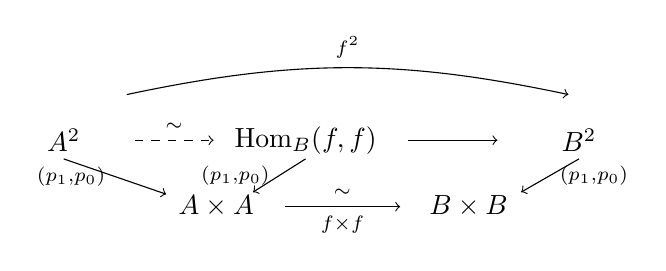
\begin{tikzpicture}[x=1.9em,y=1.5em]
  \node (a2)  at (0,1.6) {$A^{2}$};
  \node (hom) at (4.6,1.6) {$\mathrm{Hom}_{B}(f,f)$};
  \node (b2)  at (9.8,1.6) {$B^{2}$};
  \node (aa)  at (2.9,0) {$A\times A$};
  \node (bb)  at (7.7,0) {$B\times B$};
  \draw[->,dashed] (1.35,1.6) -- node[above]{$\scriptstyle\sim$} (2.85,1.6);
  \draw[->] (6.55,1.6) -- (8.25,1.6);
  \draw[->] (0,1.15) -- node[left]{$\scriptstyle(p_{1},p_{0})$} (1.95,0.3);
  \draw[->] (4.6,1.15) -- node[left]{$\scriptstyle(p_{1},p_{0})$} (3.6,0.35);
  \draw[->] (9.8,1.15) -- node[right]{$\scriptstyle(p_{1},p_{0})$} (8.7,0.35);
  \node at (5.65,0.8) {$\scriptstyle\lrcorner$};
  \draw[->] (4.2,0) -- node[above]{$\scriptstyle\sim$}
    node[below]{$\scriptstyle f\times f$} (6.4,0);
  \draw[->] (1.2,2.7) to[bend left=12] node[above]{$\scriptstyle f^{2}$} (9.6,2.7);
\end{tikzpicture}
\end{center}
本质满性是第一个等价的一个后果，而全忠实性则可沿 $A$ 的一对\trElement{}把第二
个等价拉回而得。

为证其逆，我们从把 $f$ 分解为一个\trEquivalence{}后接一个\trIsofibration{}开始。
两个因子都易于看出是逐点\trFullyFaithful{}且\trEssentiallySurjective，故
只需假设 $f\colon A\Rightarrow B$ 是一个\trIsofibration。我们现在的任务
是证明 $f$ 是一个\trTrivialFibration。在一个 $(\infty,1)$-\trCategory{}的%
\trInfinityCosmos{} $\mathcal{K}$ 中，命题 10.2.1 的宇宙论\trBiequivalence{}
$(-)_{0}\colon\mathcal{K}\Rightarrow\QCat$ 保持\trIsofibration{}并反射%
\trEquivalence。于是，为证一个\trIsofibration{} $f\colon A\Rightarrow B$
是一个\trTrivialFibration，只需证明底\trIsofibration{}
$f_{0}\colon A_{0}\Rightarrow B_{0}$ 是一个\trTrivialFibration——也就是
说，我们能够求解如下形式的\trLifting{}问题
\begin{rveq}\label{eq:trivial-fibration-lifting-fun}
\begin{tikzpicture}[x=1.9em,y=1.4em]
  \node (tl) at (0,1.4) {$\partial\Delta[n]$};
  \node (tr) at (5.6,1.4) {$\Fun(1,A)$};
  \node (bl) at (0,0) {$\Delta[n]$};
  \node (br) at (5.6,0) {$\Fun(1,B)$};
  \draw[->] (tl) -- (tr);
  \draw[right hook->] (0,0.95) -- (0,0.45);
  \draw[->,dashed] (1.0,0.25) -- (4.8,1.15);
  \draw[right hook-implies,double,double distance=0.6pt] (tr) -- node[right]{$\scriptstyle f_{0}$} (br);
  \draw[->] (bl) -- (br);
\end{tikzpicture}
\end{rveq}
对 $n\ge 0$。

在 $n=0$ 的情形，这条提升性质断言：当 $f_{0}\colon A_{0}\Rightarrow B_{0}$
是一个\trIsofibration{}时，「$f\colon A\Rightarrow B$ 是%
\trEssentiallySurjective」这一假设事实上蕴含
$f_{0}\colon A_{0}\Rightarrow B_{0}$ 在顶点上满射。由本质满性，对任何%
\trElement{} $b\colon 1\to B$，存在某个\trElement{} $a\colon 1\to A$ 使得
$fa\cong b$ 在 $\mathrm{h}B\coloneqq\mathrm{h}\Fun(1,B)\coloneqq\mathrm{h}(B_{0})$
中成立。现在，第 1 章中的\cref{cor:hc-isomorphism}蕴含：$B$ 的%
\trHomotopyCategory{}中的任何\trIsomorphism{}都可以由一个%
\trHomotopyCoherentIsomorphism{} $\qcInt\to\Fun(1,B)$ 来表示。选取一个%
\trElement{} $a\colon 1\to A$ 连同表示 $fa\cong b$ 的一个%
\trHomotopyCoherentIsomorphism{} $\beta\colon\qcInt\to\Fun(1,B)$，便定义出
如下\trLifting{}问题
\begin{center}
\begin{tikzpicture}[x=1.9em,y=1.4em]
  \node (tl) at (0,1.4) {$\varnothing$};
  \node (tm) at (3.0,1.4) {$1$};
  \node (tr) at (8.6,1.4) {$\Fun(1,A)$};
  \node (bl) at (0,0) {$1$};
  \node (bm) at (3.0,0) {$\qcInt$};
  \node (br) at (8.6,0) {$\Fun(1,B)$};
  \draw[->] (tl) -- (tm);
  \draw[->] (tm) -- node[above]{$\scriptstyle a$} (tr);
  \draw[right hook->] (0,0.95) -- (0,0.45);
  \node at (0.62,1.12) {$\scriptstyle\lrcorner$};
  \draw[right hook->] (3.0,0.95) -- (3.0,0.45);
  \draw[right hook-implies,double,double distance=0.6pt] (tr) -- node[right]{$\scriptstyle f_{0}$} (br);
  \draw[right hook->] (0.7,0) -- (2.45,0);
  \draw[->] (3.7,0) -- node[below]{$\scriptstyle\beta$} (6.4,0);
  \draw[->,dashed] (3.8,0.25) -- (7.9,1.15);
  \draw[->] (0.7,-0.8) to[bend right=15] node[below]{$\scriptstyle b$} (7.9,-0.8);
\end{tikzpicture}
\end{center}

它可以求解——沿\trIsofibration{}提升该\trIsomorphism{}即可。这就求解了
$n=0$ 情形的\trLifting{}问题 \eqref{eq:trivial-fibration-lifting-fun}。

把第 3 章中的\cref{prop:maps-between-commas}应用于左下方的交换图表，我们看到：诸\trModule{}之间的诱导映射是
一个\trIsofibration。
\begin{center}
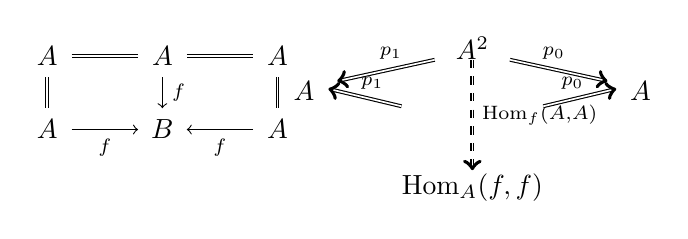
\begin{tikzpicture}[x=1.6em,y=1.4em]
  \node (a1) at (0,2.9) {$A$};
  \node (a2) at (2.6,2.9) {$A$};
  \node (a3) at (5.2,2.9) {$A$};
  \draw[double] (0.55,2.9) -- (2.05,2.9);
  \draw[double] (3.15,2.9) -- (4.65,2.9);
  \node (b1) at (0,1.0) {$A$};
  \node (b2) at (2.6,1.0) {$B$};
  \node (b3) at (5.2,1.0) {$A$};
  \draw[double] (0,2.35) -- (0,1.55);
  \draw[->] (2.6,2.35) -- node[right]{$\scriptstyle f$} (2.6,1.55);
  \draw[double] (5.2,2.35) -- (5.2,1.55);
  \draw[->] (0.55,1.0) -- node[below]{$\scriptstyle f$} (2.05,1.0);
  \draw[->] (4.65,1.0) -- node[below]{$\scriptstyle f$} (3.15,1.0);
  \node at (7.6,1.9) {$\rightsquigarrow$};
  \begin{scope}[shift={(9.6,0)}]
    \node (A2)  at (0,3.1) {$A^{2}$};
    \node (Al)  at (-3.8,2.0) {$A$};
    \node (Ar)  at (3.8,2.0) {$A$};
    \node (hb)  at (0,-0.5) {$\mathrm{Hom}_{A}(f,f)$};
    \draw[->,double,double distance=0.6pt] (-0.85,2.8) -- node[above,pos=0.45]{$\scriptstyle p_{1}$} (-3.05,2.25);
    \draw[->,double,double distance=0.6pt] (0.85,2.8) -- node[above,pos=0.45]{$\scriptstyle p_{0}$} (3.05,2.25);
    \draw[->,dashed,double,double distance=0.6pt] (0,2.8) -- node[right]{$\scriptstyle\mathrm{Hom}_{f}(A,A)$} (0,-0.05);
    \draw[->,double,double distance=0.6pt] (-1.6,1.6) -- node[above,pos=0.4]{$\scriptstyle p_{1}$} (-3.25,2.05);
    \draw[->,double,double distance=0.6pt] (1.6,1.6) -- node[above,pos=0.4]{$\scriptstyle p_{0}$} (3.25,2.05);
  \end{scope}
\end{tikzpicture}
\end{center}

由\cref{prop:fully-faithful-pointwise}，「$f$ 是逐点\trFullyFaithful」这一
假设——在诸纤维之间诱导等价
$f_{a,a'}\colon\mathrm{Hom}_{A}(a,a')\Rightarrow\mathrm{Hom}_{B}(fa,fa')$——蕴含：诱导
映射 $\mathrm{Hom}_{A}(f,f)\colon A^{2}\Rightarrow\mathrm{Hom}_{B}(f,f)$ 是一个%
\trEquivalence，从而在当前假设下是一个\trTrivialFibration。宇宙论\trFunctor{}
$(-)_{0}\colon\mathcal{K}\Rightarrow\QCat$ 把这个映射带为诸\trQuasiCategory{}%
之间的一个\trTrivialFibration，后者随之对 $n\ge 0$ 享有左下方所示的%
\trLifting{}性质：
\begin{center}
\begin{tikzpicture}[x=1.48em,y=1.7em]
  \node (tl) at (0,1.5) {$\partial\Delta[n]$};
  \node (tr) at (4.0,1.5) {$(A_{0})^{2}$};
  \node (bl) at (0,0) {$\Delta[n]$};
  \node (br) at (4.0,0) {$\mathrm{Hom}_{B_{0}}(f_{0},f_{0})$};
  \draw[->] (tl) -- (tr);
  \draw[right hook->] (0,1.05) -- (0,0.45);
  \draw[->,dashed] (0.9,0.25) -- (3.3,1.25);
  \draw[->] (tr) -- node[right,pos=0.35]{$\scriptstyle\mathrm{Hom}_{f_{0}}(A_{0},A_{0})$} (br);
  \draw[->] (bl) -- (br);
  \node at (8.0,0.75) {$\leftrightsquigarrow$};
  \begin{scope}[shift={(9.8,0)}]
    \node (tl2) at (3.6,1.8) [align=center]
      {$\partial\Delta[n]\times\Delta[1]$\\[-0.5ex]
       $\cup_{\partial\Delta[n]\times\partial\Delta[1]}$\\[-0.5ex]
       $\Delta[n]\times\partial\Delta[1]$};
    \node (tr2) at (12.4,1.8) {$A_{0}$};
    \node (bl2) at (3.6,0) {$\Delta[n]\times\Delta[1]$};
    \node (br2) at (12.4,0) {$B_{0}$};
    \draw[->] (tl2) -- (tr2);
    \draw[right hook->] (3.6,0.85) -- (3.6,0.4);
    \draw[->,dashed] (5.0,0.3) -- (11.6,1.45);
    \draw[->] (tr2) -- node[right]{$\scriptstyle f_{0}$} (br2);
    \draw[->] (bl2) -- (br2);
  \end{scope}
\end{tikzpicture}
\end{center}
经由例 A.6.14 中所给出的「逗号构造作为\trWeightedLimit{}」的描述，左上方的提升
性质穿过定义 A.6.5 的加权极限双变量伴随之 Leibniz 版本而转置，成为右上方所示的
提升性质，同样对 $n\ge 0$。

我们已经证明：$f_{0}\colon A_{0}\twoheadrightarrow B_{0}$ 也对包含
$\varnothing\hookrightarrow\Delta[0]$ 享有右提升性质。由于这个映射与 Leibniz
积包含 $(\partial\Delta[n]\hookrightarrow\Delta[n])\,\hat{\times}\,(\partial\Delta[1]\hookrightarrow\Delta[1])$
在超限复合、推出与收缩之下生成\trSimplicialSet{}的\trMonomorphism{}类，故由
「映射 $\mathrm{Hom}_{f_{0}}(A_{0},A_{0})$ 是一个\trTrivialFibration」这一事实
即知：$f_{0}\colon A_{0}\Rightarrow B_{0}$ 是一个\trTrivialFibration。
从而 $f\colon A\Rightarrow B$ 是一个\trTrivialFibration，此即所欲证。
\end{proof}

\subsection*{练习}

\begin{exercise}\label{ex:cartesian-lari-initial-elements}
用\cref{lem:opposite-qcat-biequivalence}证明\cref{prop:cocartesian-rari-terminal-elements}
与\cref{prop:fiberwise-equivalence-cartesian-functor}的对偶。
\end{exercise}

\begin{exercise}\label{ex:duals-other-results}
利用\cref{ex:cartesian-lari-initial-elements}中建立的对偶，陈述并证明本节其他
结果的对偶。
\end{exercise}

\begin{exercise}\label{ex:second-proof-absolute-right-lifting}
用\cref{cor:module-equivalence-fiberwise}给出%
\cref{prop:absolute-right-lifting-pointwise}(ii) 的第二个证明。
\end{exercise}


   %

\providecommand{\Fun}{\operatorname{Fun}}
\providecommand{\QCat}{\mathcal{Q}\mathcal{C}at}
\providecommand{\sSet}{s\mathcal{S}et}
\providecommand{\Cart}{\mathcal{C}art}
\providecommand{\coCart}{\mathit{coCart}}
\providecommand{\HomA}{\mathrm{Hom}_{A}}
\providecommand{\HomB}{\mathrm{Hom}_{B}}
\providecommand{\HomC}{\mathrm{Hom}_{C}}
\providecommand{\HomE}{\mathrm{Hom}_{E}}
\providecommand{\HomOne}{\mathrm{Hom}_{1}}

\section{逐点 Kan 扩张的存在性}\label{sec:existence-of-pointwise-kan-extensions}

有关 $(\infty,1)$-\trCategory{}论的浩瀚而又迅速扩张的文献，远远超出了本书
的范围。我们以一个示范作结，它例示了：其证明见于他处的那些结果，如何能够
被整合进∞-\trInfinityCosmos{}的「模型无关」框架之中。在本节中，我们从同行
那里借来一个结果——关乎诸\trQuasiCategory{}之间的\trCartesianFibration{}与%
\trCocartesianFibration{}的「可指数化性」——并从中汲取了相当可观的收效。

单纯集这一\trCategory，作为集合值预层的\trCategory，是\textbf{局部%
\trCartesianClosed}（locally cartesian closed）的，意即：沿单纯集之间的任何
映射 $f\colon A\to B$ 的\trPullback{}容有一个右伴随——称为「前推」
（pushforward）——以及一个由复合定义的左伴随：
\begin{rveq}\label{eq:sset-slice-adjunction}
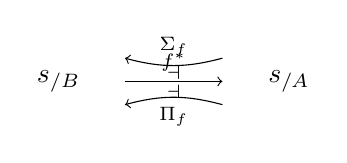
\begin{tikzpicture}[x=1.6em,y=1.5em]
  \node (lb) at (0,0)   {$s\Set_{/B}$};
  \node (rb) at (5.2,0) {$s\Set_{/A}$};
  \draw[->] (3.7,0.56) to[bend left=15] node[above,pos=0.5]{$\scriptstyle\Sigma_{f}$} (1.5,0.56);
  \node at (2.6,0.22) {$\scriptstyle\dashv$};
  \draw[->] (1.5,0) -- node[above]{$\scriptstyle f^{*}$} (3.7,0);
  \node at (2.6,-0.26) {$\scriptstyle\dashv$};
  \draw[->] (3.7,-0.56) to[bend right=15] node[below,pos=0.5]{$\scriptstyle\Pi_{f}$} (1.5,-0.56);
\end{tikzpicture}
\end{rveq}

对诸\trQuasiCategory{}之间的某些——但非全部——\trIsofibration{}
$f\colon A\twoheadrightarrow B$，这些\trAdjunction{}限制为保持%
\trIsofibration{}的\trFunctor
\begin{center}
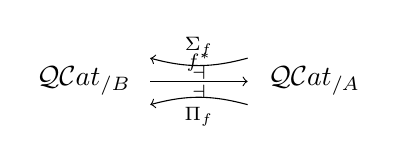
\begin{tikzpicture}[x=1.6em,y=1.5em]
  \node (lb) at (0,0)   {$\QCat_{/B}$};
  \node (rb) at (5.2,0) {$\QCat_{/A}$};
  \draw[->] (3.7,0.56) to[bend left=15] node[above,pos=0.5]{$\scriptstyle\Sigma_{f}$} (1.5,0.56);
  \node at (2.6,0.22) {$\scriptstyle\dashv$};
  \draw[->] (1.5,0) -- node[above]{$\scriptstyle f^{*}$} (3.7,0);
  \node at (2.6,-0.26) {$\scriptstyle\dashv$};
  \draw[->] (3.7,-0.56) to[bend right=15] node[below,pos=0.5]{$\scriptstyle\Pi_{f}$} (1.5,-0.56);
\end{tikzpicture}
\end{center}
此时 $f^{*}$ 与 $\Pi_{f}$ 都是宇宙论的。这样的\trIsofibration{}
$f\colon A\twoheadrightarrow B$ 称为\textbf{可指数化的}（exponentiable）。%
\footnote{一个著名的不可指数化\trFunctor{}出现于\cref{ex:nonexponentiable-d1}。}

由 Lurie 给出的、诸\trQuasiCategory{}之间可指数化\trFunctor{}的一个刻画——
他称之为「平坦纤维化」（flat fibrations）——出现于 [80, \S B.3]；一个模型
无关的刻画由 Ayala 与 Francis 给出于 [5, 2.2.8]。就我们此处的目的而言，我们
只需要：诸\trQuasiCategory{}之间的\trCocartesianFibration{}与%
\trCartesianFibration{}位列可指数化\trFunctor{}之中，而且二者分别保持%
\trCartesianFibration{}与\trCocartesianFibration。事实上，正如我们在 [114]
中所注意到的，由此得到的诸前推构造十分适配于宇宙论语境：

\begin{theorem}[{[114, 6.2.9--10]}]\label{thm:quasi-category-pushforward}
对诸\trQuasiCategory{}之间的一条\trCocartesianFibration{}
$q\colon E\twoheadrightarrow B$ 或\trCartesianFibration{}
$p\colon E\twoheadrightarrow B$，沿 $q$ 或 $p$ 的\trPullback{}容有一个右伴随，
该右伴随限制到诸宇宙论嵌入的∞-宇宙
\begin{center}
\begin{tikzpicture}[x=1.7em,y=1.6em]
  \node (qe) at (0,1.6)  {$\QCat_{/E}$};
  \node (qb) at (4.6,1.6){$\QCat_{/B}$};
  \draw[->] (3.4,2.18) to[bend left=15] node[above,pos=0.5]{$\scriptstyle q^{*}$} (1.2,2.18);
  \node at (2.3,1.82) {$\scriptstyle\dashv$};
  \draw[->] (1.2,1.02) to[bend right=15] node[below,pos=0.5]{$\scriptstyle\Pi_{q}$} (3.4,1.02);
  \node (ce) at (0,0)  {$\Cart(\QCat)_{/E}$};
  \node (cb) at (4.6,0){$\Cart(\QCat)_{/B}$};
  \draw[->] (3.3,0.44) to[bend left=15] node[above,pos=0.5]{$\scriptstyle q^{*}$} (1.3,0.44);
  \node at (2.3,0.1) {$\scriptstyle\dashv$};
  \draw[->] (1.3,-0.42) to[bend right=15] node[below,pos=0.5]{$\scriptstyle\Pi_{q}$} (3.3,-0.42);
  \draw[right hook->] (0,0.5) -- (0,1.08);
  \draw[right hook->] (4.6,0.5) -- (4.6,1.08);
  \begin{scope}[shift={(10.4,0)}]
    \node (pe) at (0,1.6)  {$\QCat_{/E}$};
    \node (pb) at (4.6,1.6){$\QCat_{/B}$};
    \draw[->] (3.4,2.18) to[bend left=15] node[above,pos=0.5]{$\scriptstyle p^{*}$} (1.2,2.18);
    \node at (2.3,1.82) {$\scriptstyle\dashv$};
    \draw[->] (1.2,1.02) to[bend right=15] node[below,pos=0.5]{$\scriptstyle\Pi_{p}$} (3.4,1.02);
    \node (oce) at (0,0)  {$\coCart(\QCat)_{/E}$};
    \node (ocb) at (4.6,0){$\coCart(\QCat)_{/B}$};
    \draw[->] (3.3,0.44) to[bend left=15] node[above,pos=0.5]{$\scriptstyle p^{*}$} (1.3,0.44);
    \node at (2.3,0.1) {$\scriptstyle\dashv$};
    \draw[->] (1.3,-0.42) to[bend right=15] node[below,pos=0.5]{$\scriptstyle\Pi_{p}$} (3.3,-0.42);
    \draw[right hook->] (0,0.5) -- (0,1.08);
    \draw[right hook->] (4.6,0.5) -- (4.6,1.08);
  \end{scope}
\end{tikzpicture}
\end{center}
之上，而且所有这些\trFunctor{}都是宇宙论的。
\end{theorem}

Lurie 关于\trCartesianFibration{}与\trCocartesianFibration{}可指数化的证明
可在 [80, B.3.11, B.4.5] 中找到；另见 [78, 3.2.2.12] 与 [80, B.4.2]。把这些
结果特例化到一个与此处所论情形远为接近的语境中，即 [115, 2.24]。

现在，我们把这些结果扩张到任意的 $(\infty,1)$-\trCategory{}的%
\trInfinityCosmos。

\begin{theorem}\label{thm:cosmos-pushforward}
对 $(\infty,1)$-\trCategory{}的\trInfinityCosmos{} $\mathcal{K}$ 中的一条%
\trCocartesianFibration{} $q\colon E\twoheadrightarrow B$ 或%
\trCartesianFibration{} $p\colon E\twoheadrightarrow B$，沿 $q$ 或 $p$ 的%
\trPullback{}容有一个拟伪函子性的右双伴随，该右双伴随限制到诸宇宙论嵌入的
∞-宇宙
\begin{center}
\begin{tikzpicture}[x=1.7em,y=1.6em]
  \node (ke) at (0,1.6)  {$\mathcal{K}_{/E}$};
  \node (kb) at (4.6,1.6){$\mathcal{K}_{/B}$};
  \draw[->] (3.4,2.18) -- ++(-0.36,0.07) -- ++(-0.36,-0.14) -- ++(-0.36,0.14)
    -- ++(-0.36,-0.14) -- ++(-0.36,0.14) -- ++(-0.36,-0.14) -- ++(-0.37,0.07);
  \node at (2.3,2.5) {$\scriptstyle q^{*}$};
  \node at (2.3,1.82) {$\scriptstyle\dashv$};
  \draw[->] (1.2,1.02) -- ++(0.36,-0.07) -- ++(0.36,0.14) -- ++(0.36,-0.14)
    -- ++(0.36,0.14) -- ++(0.36,-0.14) -- ++(0.36,0.14) -- ++(0.37,-0.07);
  \node at (2.3,0.68) {$\scriptstyle\Pi_{q}$};
  \node (ce) at (0,0)  {$\Cart(\mathcal{K})_{/E}$};
  \node (cb) at (4.6,0){$\Cart(\mathcal{K})_{/B}$};
  \draw[->] (3.3,0.44) -- ++(-0.33,0.07) -- ++(-0.33,-0.14) -- ++(-0.33,0.14)
    -- ++(-0.33,-0.14) -- ++(-0.33,0.14) -- ++(-0.34,0.07);
  \node at (2.3,0.72) {$\scriptstyle q^{*}$};
  \node at (2.3,0.1) {$\scriptstyle\dashv$};
  \draw[->] (1.3,-0.42) -- ++(0.33,-0.07) -- ++(0.33,0.14) -- ++(0.33,-0.14)
    -- ++(0.33,0.14) -- ++(0.33,-0.14) -- ++(0.34,0.07);
  \node at (2.3,-0.72) {$\scriptstyle\Pi_{q}$};
  \draw[right hook->] (0,0.5) -- (0,1.08);
  \draw[right hook->] (4.6,0.5) -- (4.6,1.08);
  \begin{scope}[shift={(10.4,0)}]
    \node (pe) at (0,1.6)  {$\mathcal{K}_{/E}$};
    \node (pb) at (4.6,1.6){$\mathcal{K}_{/B}$};
    \draw[->] (3.4,2.18) -- ++(-0.36,0.07) -- ++(-0.36,-0.14) -- ++(-0.36,0.14)
      -- ++(-0.36,-0.14) -- ++(-0.36,0.14) -- ++(-0.36,-0.14) -- ++(-0.37,0.07);
    \node at (2.3,2.5) {$\scriptstyle p^{*}$};
    \node at (2.3,1.82) {$\scriptstyle\dashv$};
    \draw[->] (1.2,1.02) -- ++(0.36,-0.07) -- ++(0.36,0.14) -- ++(0.36,-0.14)
      -- ++(0.36,0.14) -- ++(0.36,-0.14) -- ++(0.36,0.14) -- ++(0.37,-0.07);
    \node at (2.3,0.68) {$\scriptstyle\Pi_{p}$};
    \node (oce) at (0,0)  {$\coCart(\mathcal{K})_{/E}$};
    \node (ocb) at (4.6,0){$\coCart(\mathcal{K})_{/B}$};
    \draw[->] (3.3,0.44) -- ++(-0.33,0.07) -- ++(-0.33,-0.14) -- ++(-0.33,0.14)
      -- ++(-0.33,-0.14) -- ++(-0.33,0.14) -- ++(-0.34,0.07);
    \node at (2.3,0.72) {$\scriptstyle p^{*}$};
    \node at (2.3,0.1) {$\scriptstyle\dashv$};
    \draw[->] (1.3,-0.42) -- ++(0.33,-0.07) -- ++(0.33,0.14) -- ++(0.33,-0.14)
      -- ++(0.33,0.14) -- ++(0.33,-0.14) -- ++(0.34,0.07);
    \node at (2.3,-0.72) {$\scriptstyle\Pi_{p}$};
    \draw[right hook->] (0,0.5) -- (0,1.08);
    \draw[right hook->] (4.6,0.5) -- (4.6,1.08);
  \end{scope}
\end{tikzpicture}
\end{center}
之上，

而陈述中的「双伴随性」——再次挪用弱 2-范畴论的一个术语——意指一个拟伪自然
的\trEquivalence：
\begin{center}
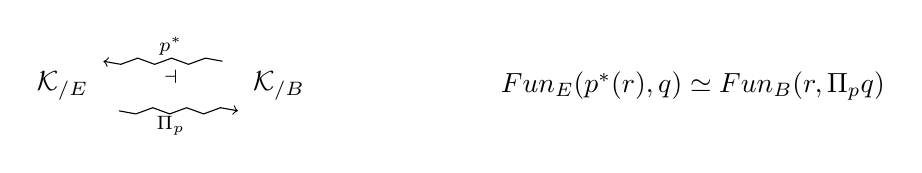
\begin{tikzpicture}[x=1.7em,y=1.6em]
  \node (ke) at (0,0)  {$\mathcal{K}_{/E}$};
  \node (kb) at (4.6,0){$\mathcal{K}_{/B}$};
  \draw[->] (3.4,0.56) -- ++(-0.36,0.07) -- ++(-0.36,-0.14) -- ++(-0.36,0.14)
    -- ++(-0.36,-0.14) -- ++(-0.36,0.14) -- ++(-0.36,-0.14) -- ++(-0.37,0.07);
  \node at (2.3,0.9) {$\scriptstyle p^{*}$};
  \node at (2.3,0.22) {$\scriptstyle\dashv$};
  \draw[->] (1.2,-0.56) -- ++(0.36,-0.07) -- ++(0.36,0.14) -- ++(0.36,-0.14)
    -- ++(0.36,0.14) -- ++(0.36,-0.14) -- ++(0.36,0.14) -- ++(0.37,-0.07);
  \node at (2.3,-0.9) {$\scriptstyle\Pi_{p}$};
  \node at (13.4,0) {$\Fun_{E}(p^{*}(r),q)\simeq\Fun_{B}(r,\Pi_{p}q)$};
\end{tikzpicture}
\end{center}
\end{theorem}

\begin{proof}
对一条余/笛卡尔纤维化 $p\colon E\twoheadrightarrow B$，前推拟伪函子
$\Pi_{p}\colon\mathcal{K}_{/E}\rightsquigarrow\mathcal{K}_{/B}$ 定义为：与
介于诸\trQuasiCategory{}之间的底余/笛卡尔纤维化
$p_{0}\colon E_{0}\to B_{0}$ 相关联的前推，与宇宙论双等价的之字形链

\begin{rveq}\label{eq:pushforward-slice-zigzag}
\begin{tikzpicture}[x=1.6em,y=1.5em]
  \node (ke)  at (0,1.5)   {$\mathcal{K}_{/E}$};
  \node (kb)  at (4.6,1.5) {$\mathcal{K}_{/B}$};
  \draw[->] (1.1,1.5) -- ++(0.42,0.07) -- ++(0.42,-0.14) -- ++(0.42,0.14)
    -- ++(0.42,-0.14) -- ++(0.42,0.14) -- ++(0.42,-0.14) -- ++(0.43,0.07);
  \node at (2.85,1.92) {$\scriptstyle\Pi_{p}$};
  \draw[->] (0,1.0) -- node[left]{$\scriptstyle(-)_{0}$} (0,0.5);
  \node at (2.3,0.78) {$\scriptstyle\simeq$};
  \draw[right hook->] (4.6,1.0) -- node[right]{$\scriptstyle(-)_{0}$} (4.6,0.5);
  \node (qe) at (0,0)   {$\QCat_{/E_{0}}$};
  \node (qb) at (4.6,0) {$\QCat_{/B_{0}}$};
  \draw[->] (1.1,0) -- node[below]{$\scriptstyle\Pi_{p_{0}}$} (3.5,0);
\end{tikzpicture}
\end{rveq}
给出的。注意：\trPullback{}与前推二者都与切片化的底拟范畴\trFunctor{}
$(-)_{0}\colon\mathcal{K}_{/B}\Rightarrow\QCat_{/B_{0}}$ 在等价的意义下
交换。

依据下列复合\trEquivalence，这个复合拟伪函子可以理解为一个逐点的右双伴随
\[
\begin{gathered}
\Fun_{E}(p^{*}(r),q)\xrightarrow{\;(-)_{0}\;}\Fun_{E_{0}}((p_{0})^{*}(r_{0}),q_{0})\\
\parallel\\
\Fun_{B_{0}}(r_{0},\Pi_{p_{0}}(q_{0}))\xleftarrow{\;(-)_{0}\;}\Fun_{B}(r,\Pi_{p}q)
\end{gathered}
\]
它们在 $q\colon F\twoheadrightarrow E$ 与 $r\colon G\twoheadrightarrow B$ 中
是拟伪自然地定义的。这就证明了第一款陈述。

现在，设 $p\colon E\twoheadrightarrow B$ 是 $\mathcal{K}$ 中的一条%
\trCartesianFibration，并设 $q\colon F\twoheadrightarrow E$ 是一条%
\trCocartesianFibration。那么由第 10 章中的命题 10.3.6，$\Pi_{p}q$ 是
$\mathcal{K}$ 中的\trCocartesianFibration，当且仅当其底\trFunctor{}是诸%
\trQuasiCategory{}上的\trCocartesianFibration。由 \eqref{eq:pushforward-slice-zigzag}
的本质交换性，这个\trFunctor{}等价于 $\Pi_{p_{0}}(q_{0})$，而由%
\cref{thm:quasi-category-pushforward}，后者是诸\trQuasiCategory{}的一条%
\trCocartesianFibration。由于余笛卡尔纤维化性在等价之下是重满的，保持结果
随之而来。前推保持笛卡尔函子的证明类似地成立。

最后，\cref{thm:quasi-category-pushforward}证明：诸\trQuasiCategory{}的余笛卡尔
纤维化之间的\trCartesianFunctor{}在 $p^{*}\dashv\Pi_{p}$ 之下转置为笛卡尔
函子。由于\trCartesianFunctor{}被诸宇宙论双等价保持并反射，同样的事情在任何
$(\infty,1)$-\trCategory{}的\trInfinityCosmos{}中成立。于是，拟伪自然的%
\trEquivalence{} $\Fun_{E}(p^{*}(r),q)\simeq\Fun_{B}(r,\Pi_{p}q)$ 限制而定义
一个拟伪自然的\trEquivalence{}
$\Fun^{\mathit{cart}}_{E}(p^{*}(r),q)\simeq\Fun^{\mathit{cart}}_{B}(r,\Pi_{p}q)$。
\end{proof}


\begin{lemma}[Beck--Chevalley]\label{lem:beck-chevalley-qcat}
考虑 $(\infty,1)$-\trCategory{}的\trInfinityCosmos{}中的一个\trPullback{}图
\begin{center}
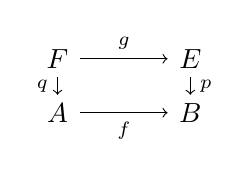
\begin{tikzpicture}[x=1.5em,y=1.3em]
  \node (f) at (0,1.5) {$F$};
  \node (e) at (3.2,1.5) {$E$};
  \node (a) at (0,0)   {$A$};
  \node (b) at (3.2,0) {$B$};
  \draw[->] (0.55,1.5) -- node[above]{$\scriptstyle g$} (2.65,1.5);
  \draw[->] (0,1.0) -- node[left]{$\scriptstyle q$} (0,0.5);
  \draw[->] (3.2,1.0) -- node[right]{$\scriptstyle p$} (3.2,0.5);
  \draw[->] (0.55,0) -- node[below]{$\scriptstyle f$} (2.65,0);
  \node at (0.62,0.95) {$\scriptstyle\lrcorner$};
\end{tikzpicture}
\end{center}
并设 $p$ 是一条\trCocartesianFibration{}或\trCartesianFibration。那么对一切
$r\colon G\twoheadrightarrow E$，诸映射
$f^{*}\Pi_{p}r\simeq\Pi_{q}g^{*}r$ 在 $A$ 之上等价。
\end{lemma}

\begin{proof}
施用宇宙论双等价 $(-)_{0}\colon\mathcal{K}\Rightarrow\QCat$，只需对诸%
\trQuasiCategory{}证明本引理；此时所论的诸\trFunctor{}容有左伴随：
\begin{center}
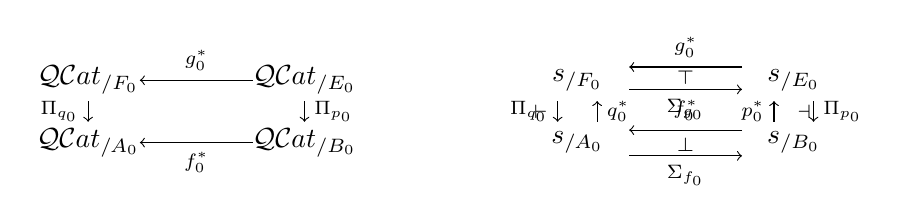
\begin{tikzpicture}[x=1.7em,y=1.5em]
  \node (a) at (0,1.5)  {$\QCat_{/F_{0}}$};
  \node (b) at (4.6,1.5){$\QCat_{/E_{0}}$};
  \draw[->] (3.5,1.5) -- node[above]{$\scriptstyle g_{0}^{*}$} (1.1,1.5);
  \draw[->] (0,1.0) -- node[left]{$\scriptstyle\Pi_{q_{0}}$} (0,0.5);
  \draw[->] (4.6,1.0) -- node[right]{$\scriptstyle\Pi_{p_{0}}$} (4.6,0.5);
  \node (c) at (0,0)  {$\QCat_{/A_{0}}$};
  \node (d) at (4.6,0){$\QCat_{/B_{0}}$};
  \draw[->] (3.5,0) -- node[below]{$\scriptstyle f_{0}^{*}$} (1.1,0);
  \begin{scope}[shift={(10.4,0)}]
    \node (a2) at (0,1.5)  {$s\Set_{/F_{0}}$};
    \node (b2) at (4.6,1.5){$s\Set_{/E_{0}}$};
    \draw[->] (3.5,1.82) -- node[above]{$\scriptstyle g_{0}^{*}$} (1.1,1.82);
    \node at (2.3,1.56) {$\scriptstyle\top$};
    \draw[->] (1.1,1.28) -- node[below]{$\scriptstyle\Sigma_{g_{0}}$} (3.5,1.28);
    \draw[->] (-0.42,1.0) -- node[left]{$\scriptstyle\Pi_{q_{0}}$} (-0.42,0.5);
    \node at (-0.78,0.75) {$\scriptstyle\vdash$};
    \draw[->] (0.42,0.5) -- node[right]{$\scriptstyle q_{0}^{*}$} (0.42,1.0);
    \draw[->] (4.18,0.5) -- node[left]{$\scriptstyle p_{0}^{*}$} (4.18,1.0);
    \node at (4.82,0.75) {$\scriptstyle\dashv$};
    \draw[->] (5.02,1.0) -- node[right]{$\scriptstyle\Pi_{p_{0}}$} (5.02,0.5);
    \node (c2) at (0,0)  {$s\Set_{/A_{0}}$};
    \node (d2) at (4.6,0){$s\Set_{/B_{0}}$};
    \draw[->] (1.1,-0.32) -- node[below]{$\scriptstyle\Sigma_{f_{0}}$} (3.5,-0.32);
    \node at (2.3,-0.06) {$\scriptstyle\perp$};
    \draw[->] (3.5,0.3) -- node[above]{$\scriptstyle f_{0}^{*}$} (1.1,0.3);
  \end{scope}
\end{tikzpicture}
\end{center}

对单纯集之间的任何映射 $a\colon X\to A_{0}$，通过检视如下\trPullback{}矩形
\begin{center}
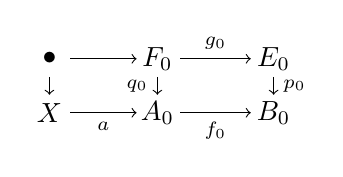
\begin{tikzpicture}[x=1.5em,y=1.3em]
  \node (x1) at (0,1.5)  {$\bullet$};
  \node (f0) at (2.6,1.5){$F_{0}$};
  \node (e0) at (5.4,1.5){$E_{0}$};
  \node (x2) at (0,0)    {$X$};
  \node (a0) at (2.6,0)  {$A_{0}$};
  \node (b0) at (5.4,0)  {$B_{0}$};
  \draw[->] (0.5,1.5) -- (2.1,1.5);
  \draw[->] (3.15,1.5) -- node[above]{$\scriptstyle g_{0}$} (4.85,1.5);
  \draw[->] (0,1.0) -- (0,0.5);
  \draw[->] (2.6,1.0) -- node[left]{$\scriptstyle q_{0}$} (2.6,0.5);
  \draw[->] (5.4,1.0) -- node[right]{$\scriptstyle p_{0}$} (5.4,0.5);
  \draw[->] (0.5,0) -- node[below]{$\scriptstyle a$} (2.1,0);
  \draw[->] (3.15,0) -- node[below]{$\scriptstyle f_{0}$} (4.85,0);
  \node at (2.05,0.98) {$\scriptstyle\lrcorner$};
  \node at (3.18,0.98) {$\scriptstyle\lrcorner$};
\end{tikzpicture}
\end{center}
显然有 $\Sigma_{g_{0}}q_{0}^{*}a\cong p_{0}^{*}\Sigma_{f_{0}}a$。于是，右伴随
$f_{0}^{*}\Pi_{p_{0}}\cong\Pi_{q_{0}}g_{0}^{*}$ 也在\trIsomorphism{}的意义下
交换，而保守性给出 $\mathcal{K}$ 中所宣称的\trEquivalence。
\end{proof}

现在我们来解释我们对这些结果的兴趣所在。由第 9 章中的%
\cref{def:right-extension-lifting-modules}回忆起：模 $A\xrightarrow{G}C$ 沿模
$A\xrightarrow{E}B$ 的一个\textbf{右扩张}，由一个数对给出——其中一支模
$B\xrightarrow{\hom_{A}(E,G)}C$ 连同一支二元\trCell
\begin{center}
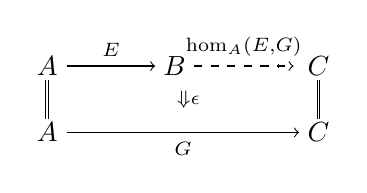
\begin{tikzpicture}[x=1em,y=1em]
  \node at (0,1.2)    {$A$};
  \node at (4.6,1.2)  {$B$};
  \node at (9.8,1.2)  {$C$};
  \node at (0,-1.2)   {$A$};
  \node at (9.8,-1.2) {$C$};
  \draw[->] (0.7,1.2)  -- node[above]{$\scriptstyle E$} (3.9,1.2);
  \draw[->,dashed] (5.3,1.2) -- node[above]{$\scriptstyle\hom_{A}(E,G)$} (8.9,1.2);
  \draw (8.35,1.12) -- (8.35,1.28);
  \draw[->] (0.7,-1.2) -- node[below]{$\scriptstyle G$} (9.1,-1.2);
  \draw[double,double distance=0.6pt] (0,0.7)   -- (0,-0.7);
  \draw[double,double distance=0.6pt] (9.8,0.7) -- (9.8,-0.7);
  \node at (5.1,0) {$\scriptstyle\Downarrow\epsilon$};
\end{tikzpicture}
\end{center}
构成，该\trCell{}在模的\trVirtualEquipment{}中的诸\trCell{}之间按彼处详述的
意义是泛的。对偶地，$A\xrightarrow{G}C$ 穿过 $B\xrightarrow{F}C$ 的一个%
\textbf{右提升}，由一个数对给出——其中一支模
$A\xrightarrow{\hom(F,G)_{C}}B$ 连同一支泛的二元\trCell
\begin{center}
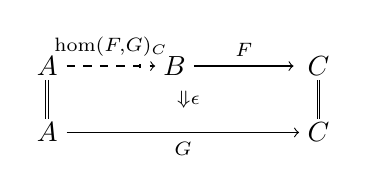
\begin{tikzpicture}[x=1em,y=1em]
  \node at (0,1.2)    {$A$};
  \node at (4.6,1.2)  {$B$};
  \node at (9.8,1.2)  {$C$};
  \node at (0,-1.2)   {$A$};
  \node at (9.8,-1.2) {$C$};
  \draw[->,dashed] (0.7,1.2) -- node[above]{$\scriptstyle\hom(F,G)_{C}$} (3.9,1.2);
  \draw (3.35,1.12) -- (3.35,1.28);
  \draw[->] (5.3,1.2)  -- node[above]{$\scriptstyle F$} (8.9,1.2);
  \draw[->] (0.7,-1.2) -- node[below]{$\scriptstyle G$} (9.1,-1.2);
  \draw[double,double distance=0.6pt] (0,0.7)   -- (0,-0.7);
  \draw[double,double distance=0.6pt] (9.8,0.7) -- (9.8,-0.7);
  \node at (5.1,0) {$\scriptstyle\Downarrow\epsilon$};
\end{tikzpicture}
\end{center}
构成。此处我们为这些概念引入不同的记号，意在给它们改换名目。我们把模
$\hom_{A}(E,G)$ 称为从 $E$ 到 $G$ 的\textbf{左 hom}（left hom）\footnote{原书
此处行文作「the left hom from $E$ to $F$」，且 p.489 右扩张展示图之第二模标签
亦印作 $\hom_{A}(E,F)$；按本条首句（结果模为 $\hom_{A}(E,G)$）与下句
「homomorphisms from $E$ to $G$」，两处 $F$ 均系 $G$ 之误，径改。——译者注}，把
$\hom(F,G)_{C}$ 称为从 $F$ 到 $G$ 的\textbf{右 hom}（right hom）。延伸
「模」这一隐喻，我们把左 hom 设想为从 $E$ 到 $G$ 的、尊重左 $A$-作用的诸%
\trHomomorphism{}之对象，而右 hom 则是从 $F$ 到 $G$ 的、尊重右 $C$-作用的诸\trHomomorphism{}之对象。
我们本节的第一个目标，是论证诸\trQuasiCategory{}之间的模的%
\trVirtualEquipment{}对一切合适的模对都拥有左 hom 与右 hom。由%
\trModelIndependence，这一结果扩张到任何 $(\infty,1)$-\trCategory{}的%
\trInfinityCosmos。

\begin{theorem}\label{thm:module-equipment-biclosed}
诸\trQuasiCategory{}之间的模的\trVirtualEquipment{}是\textbf{双闭的}
（biclosed），容有满足一个富集\trUniversalProperty{}的左 hom 与右 hom：对模
$A\xrightarrow{E}B$、$B\xrightarrow{F}C$ 与 $A\xrightarrow{G}C$，
\[
\Fun_{A\times B}\bigl(E,\hom(F,G)_{C}\bigr)\cong
\Fun_{A\times C}(E\times_{B}F,G)\cong
\Fun_{B\times C}\bigl(F,\hom_{A}(E,G)\bigr).
\]
\end{theorem}

\begin{proof}
左 hom 与右 hom 的情形是对偶的，故我们聚焦于前者。固定一条模
$A\overset{q}{\twoheadleftarrow}E\overset{p}{\twoheadrightarrow}B$，把
$\hom_{A}(E,G)$ 定义为模 $A\xrightarrow{G}C$ 在下列复合右伴随\trFunctor{}%
之下的像：
\begin{center}
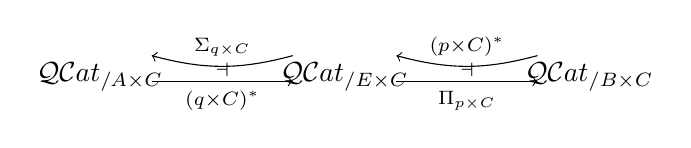
\begin{tikzpicture}[x=1.7em,y=1.5em]
  \node (a) at (0,0)    {$\QCat_{/A\times C}$};
  \node (b) at (5.2,0)  {$\QCat_{/E\times C}$};
  \node (c) at (10.4,0) {$\QCat_{/B\times C}$};
  \draw[->] (4.1,0.52) to[bend left=15] node[above,pos=0.5]{$\scriptstyle\Sigma_{q\times C}$} (1.1,0.52);
  \node at (2.6,0.18) {$\scriptstyle\dashv$};
  \draw[->] (1.1,-0.1) -- node[below]{$\scriptstyle(q\times C)^{*}$} (4.1,-0.1);
  \draw[->] (9.3,0.52) to[bend left=15] node[above,pos=0.5]{$\scriptstyle(p\times C)^{*}$} (6.3,0.52);
  \node at (7.8,0.18) {$\scriptstyle\dashv$};
  \draw[->] (6.3,-0.1) -- node[below]{$\scriptstyle\Pi_{p\times C}$} (9.3,-0.1);
\end{tikzpicture}
\end{center}
注意：该左伴随把双侧等价纤维化
$B\overset{s}{\twoheadleftarrow}F\overset{r}{\twoheadrightarrow}C$ 带为复合
双侧等价纤维化
\begin{center}
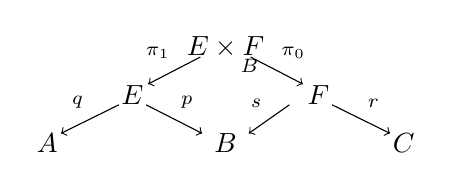
\begin{tikzpicture}[x=1.4em,y=1.15em]
  \node (ef) at (0,3.0)  {$E\times F$};
  \node at (0.62,2.42)   {$\scriptstyle B$};
  \node (e)  at (-2.4,1.5){$E$};
  \node (f)  at (2.4,1.5) {$F$};
  \node (a)  at (-4.6,0)  {$A$};
  \node (b)  at (0,0)     {$B$};
  \node (c)  at (4.6,0)   {$C$};
  \draw[->] (-0.65,2.7) -- node[above left,pos=0.4]{$\scriptstyle\pi_{1}$} (-2.0,1.85);
  \draw[->] (0.65,2.7)  -- node[above right,pos=0.4]{$\scriptstyle\pi_{0}$} (2.0,1.85);
  \node at (0.35,2.2) {$\scriptstyle\lrcorner$};
  \draw[->] (-2.75,1.2) -- node[above left,pos=0.45]{$\scriptstyle q$} (-4.25,0.3);
  \draw[->] (-2.05,1.2) -- node[above right,pos=0.45]{$\scriptstyle p$} (-0.6,0.3);
  \draw[->] (1.65,1.2)  -- node[above left,pos=0.45]{$\scriptstyle s$} (0.6,0.3);
  \draw[->] (2.75,1.2)  -- node[above right,pos=0.45]{$\scriptstyle r$} (4.25,0.3);
\end{tikzpicture}
\end{center}
而单纯富集的伴随性给出诸\trQuasiCategory{}之间的自然等价（在此情形中即%
\trIsomorphism）
\[
\Fun_{A\times C}(E\times_{B}F,G)\cong
\Fun_{B\times C}\bigl(F,\hom_{A}(E,G)\bigr).
\]

这些\trEquivalence{}在这些\trQuasiCategory{}的对象的同构类之集合上诱导双射。
由第 8 章中的命题 8.1.6，这就给出了右 hom 在模的\trVirtualEquipment{}中所需
的\trUniversalProperty（见\cref{ex:module-cell-right-extension}）——至少一旦我们证明了：当 $E$ 与 $G$
是模时，$\hom_{A}(E,G)$ 定义一条模。

于是，尚待证明的只是：当 $A\xrightarrow{E}B$
是一条模时，\trFunctor
\[
\hom_{A}(E,-)\colon\QCat_{/A\times C}
  \xrightarrow{\;(q\times C)^{*}\;}\QCat_{/E\times C}
  \xrightarrow{\;\Pi_{p\times C}\;}\QCat_{/B\times C}
\]
保持模。

第 7 章中的命题 7.4.5 告诉我们：模在\trPullback{}之下稳定，故我们只需论证：
$\Pi_{p\times C}$ 把一条模
$E\overset{v}{\twoheadleftarrow}M\overset{u}{\twoheadrightarrow}C$ 带为一条
从 $B$ 到 $C$ 的模。第 7 章中的命题 7.4.2 把从 $E$ 到 $C$ 的模刻画为那些满足
如下条件的双侧等价纤维化 $(v,u)\colon M\twoheadrightarrow E\times C$：
\begin{enumerate}[label=(\roman*)]
\item $(v,u)\colon M\twoheadrightarrow E\times C$ 是 $\QCat_{/C}$ 中的一条%
  \trCocartesianFibration，
\item $(v,u)\colon M\twoheadrightarrow E\times C$ 是 $\QCat_{/E}$ 中的一条%
  \trCartesianFibration，
\item $(v,u)\colon M\twoheadrightarrow E\times C$ 作为 $\QCat_{/E\times C}$
  中的对象是\trDiscrete。
\end{enumerate}
我们将证明 $\Pi_{p\times C}$ 保持这些性质中的每一条，从而断定 $\Pi_{p\times C}M$
定义一条从 $B$ 到 $C$ 的模。(iii) 的保持是自动的：\cref{thm:quasi-category-pushforward}
表明前推是一个宇宙论\trFunctor，而第 1 章中的%
\cref{rem:cosmological-discrete-categories}观察到宇宙论\trFunctor{}保持%
\trDiscrete{}对象。

为证 (ii)，我们必须证明 $\Pi_{p\times C}M\twoheadrightarrow B\times C$ 是
$\QCat_{/B}$ 中的一条\trCartesianFibration。首先，由第 10 章中的命题 10.1.4
注意到：宇宙论\trFunctor{} $\Pi_{p}\colon\QCat_{/E}\to\QCat_{/B}$ 保持%
\trCartesianFibration，\footnote{这并非\cref{thm:cosmos-pushforward}的一个
应用——在该语境中，\cref{thm:cosmos-pushforward}会告诉我们 $\Pi_{p}$ 把
$E$ 之上的一条\trCocartesianFibration{}带到 $B$ 之上的一条%
\trCocartesianFibration。不如说，我们注意到：$\Pi_{p}$ 仅凭其为宇宙论的这
一点，就把介于余定义域为 $E$ 的诸\trIsofibration{}之间的%
\trCartesianFibration，带为介于余定义域为 $B$ 的诸\trIsofibration{}之间的%
\trCartesianFibration。}于是我们断定 $\Pi_{p}M\twoheadrightarrow\Pi_{p}(B\times C)$
是 $\QCat_{/B}$ 中的一条\trCartesianFibration。然而，这个\trFunctor{}与
$\Pi_{p\times C}M\twoheadrightarrow B\times C$ 并不重合。不如说，正如下面的
\cref{lem:pushforward-image-pullback}所证明的，$\Pi_{p\times C}M\twoheadrightarrow B\times C$
是 $\Pi_{p}M\twoheadrightarrow\Pi_{p}(B\times C)$ 在 $\QCat_{/B}$ 中的一个%
\trPullback，故由\trCartesianFibration{}的拉回稳定性，这就证明了 (ii)。

为证余下的性质 (i)，由第 7 章中的\cref{lem:cartesian-on-the-right}回忆起：
说 $(v,u)\colon M\twoheadrightarrow E\times C$ 定义 $\QCat_{/C}$ 中的一条%
\trCocartesianFibration，等价于说 $(v,u)\colon M\twoheadrightarrow E\times C$
在子∞-宇宙 $\coCart(\QCat)_{/E}\subset\QCat_{/E}$ 中定义一个态射。由%
\cref{thm:quasi-category-pushforward}，前推限制而定义一个宇宙论\trFunctor{}
$\Pi_{p}\colon\coCart(\QCat)_{/E}\to\coCart(\QCat)_{/B}$，故
$\Pi_{p}M\twoheadrightarrow\Pi_{p}(E\times C)$ 居于子宇宙
$\coCart(\QCat)_{/B}\subset\QCat_{/B}$ 之中。由于\trPullback{}由宇宙论嵌入
$\coCart(\QCat)_{/B}\hookrightarrow\QCat_{/B}$ 所创造，由%
\cref{lem:pushforward-image-pullback}，$\Pi_{p\times C}M\twoheadrightarrow B\times C$
也居于子宇宙 $\coCart(\QCat)_{/B}\subset\QCat_{/B}$ 之中。于是，第 7 章中的%
\cref{lem:cartesian-on-the-right}告诉我们：$\Pi_{p\times C}M\twoheadrightarrow B\times C$
是 $\QCat_{/C}$ 中的一条\trCocartesianFibration，如所需。
\end{proof}

\begin{lemma}\label{lem:pushforward-image-pullback}
设 $p\colon E\twoheadrightarrow B$ 是诸\trQuasiCategory{}之间的一条%
\trCartesianFibration{}或\trCocartesianFibration。那么，一条\trIsofibration{}
$M\twoheadrightarrow E\times C$ 在
$\Pi_{p\times C}\colon\QCat_{/E\times C}\to\QCat_{/B\times C}$ 之下的像，就是
由如下\trPullback
\begin{center}
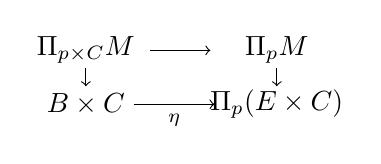
\begin{tikzpicture}[x=1.5em,y=1.3em]
  \node (tl) at (0,1.5)  {$\Pi_{p\times C}M$};
  \node (tr) at (4.6,1.5){$\Pi_{p}M$};
  \node (bl) at (0,0)    {$B\times C$};
  \node (br) at (4.6,0)  {$\Pi_{p}(E\times C)$};
  \draw[->] (1.55,1.5) -- (3.0,1.5);
  \draw[->] (0,1.0) -- (0,0.5);
  \draw[->] (4.6,1.0) -- (4.6,0.5);
  \draw[->] (1.15,0) -- node[below]{$\scriptstyle\eta$} (3.1,0);
  \node at (0.62,0.95) {$\scriptstyle\lrcorner$};
\end{tikzpicture}
\end{center}
所定义的左侧竖直\trIsofibration，其中右侧的竖直态射是映射
$M\twoheadrightarrow E\times C$ 在
$\Pi_{p}\colon\QCat_{/E}\to\QCat_{/B}$ 之下的像。
\end{lemma}

引理 12.3.7 的结论在等价意义下对任何 $(\infty,1)$-\trCategory{}的%
\trInfinityCosmos{} $\mathcal{K}$ 都成立（见\cref{ex:model-independent-lemma-12-3-7}）。然而我们发现，
与\cref{thm:cosmos-pushforward}的较弱伴随打交道，不如与%
\cref{thm:quasi-category-pushforward}的严格伴随打交道来得容易。

\begin{proof}
为使陈述有意义，注意到 $p^{*}$ 把 $\pi\colon B\times C\twoheadrightarrow B$
带为 $\pi\colon E\times C\twoheadrightarrow E$。于是，映射
$\eta\colon B\times C\to\Pi_{p}(E\times C)$ 是\trAdjunction{}
$p^{*}\dashv\Pi_{p}$ 的\trUnit{}的一个分量。现在，通过验证所示\trPullback{}%
具有定义 $\Pi_{p\times C}M\in\QCat_{/B\times C}$ 的那个\trUniversalProperty，
断言便直接得出。\trPullback{}图上的一个\trCone{}可以解读为 $\QCat_{/B}$ 中的
一个\trDiagram
\begin{center}
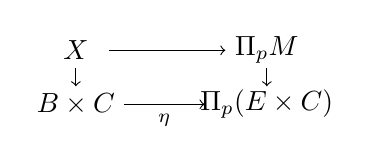
\begin{tikzpicture}[x=1.5em,y=1.3em]
  \node (tl) at (0,1.5) {$X$};
  \node (tr) at (4.6,1.5){$\Pi_{p}M$};
  \node (bl) at (0,0)   {$B\times C$};
  \node (br) at (4.6,0) {$\Pi_{p}(E\times C)$};
  \draw[->] (0.8,1.5) -- (3.6,1.5);
  \draw[->] (0,1.0) -- (0,0.5);
  \draw[->] (4.6,1.0) -- (4.6,0.5);
  \draw[->] (1.15,0) -- node[below]{$\scriptstyle\eta$} (3.1,0);
\end{tikzpicture}
\end{center}
后者转置而定义 $\QCat_{/E}$ 中的一个交换方块
\begin{center}
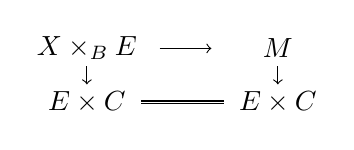
\begin{tikzpicture}[x=1.5em,y=1.3em]
  \node (tl) at (0,1.5) {$X\times_{B}E$};
  \node (tr) at (4.6,1.5){$M$};
  \node (bl) at (0,0)   {$E\times C$};
  \node (br) at (4.6,0) {$E\times C$};
  \draw[->] (1.75,1.5) -- (3.0,1.5);
  \draw[->] (0,1.0) -- (0,0.5);
  \draw[->] (4.6,1.0) -- (4.6,0.5);
  \draw[double,double distance=0.6pt] (1.3,0) -- (3.3,0);
\end{tikzpicture}
\end{center}
事实上，这个\trDiagram{}居于 $\QCat_{/E\times C}$ 之中，且左侧的竖直映射
$X\times_{B}E\twoheadrightarrow E\times C$ \trIsomorphism{}于
$(p\times C)^{*}(X\twoheadrightarrow B\times C)$。于是，这个方块沿
$(p\times C)^{*}\dashv\Pi_{p\times C}$ 转置为一个交换方块
\begin{center}
\begin{tikzpicture}[x=1.5em,y=1.3em]
  \node (tl) at (0,1.5) {$X$};
  \node (tr) at (4.6,1.5){$\Pi_{p\times C}M$};
  \node (bl) at (0,0)   {$B\times C$};
  \node (br) at (4.6,0) {$B\times C$};
  \draw[->] (0.8,1.5) -- (3.4,1.5);
  \draw[->] (0,1.0) -- (0,0.5);
  \draw[->] (4.6,1.0) -- (4.6,0.5);
  \draw[double,double distance=0.6pt] (1.3,0) -- (3.3,0);
\end{tikzpicture}
\end{center}
这就证明了断言。
\end{proof}

定理 12.3.6 的结果扩张到相互双等价的∞-宇宙：

\begin{corollary}\label{cor:module-equipment-biclosed-cosmos}
在一个 $(\infty,1)$-\trCategory{}的\trInfinityCosmos{}中，模的%
\trVirtualEquipment{}是双闭的，容有满足一个\emph{弱}富集\trUniversalProperty{}%
的左 hom 与右 hom：对模
$A\xrightarrow{E}B$、$B\xrightarrow{F}C$ 与 $A\xrightarrow{G}C$，
\[
\Fun_{A\times B}\bigl(E,\hom(F,G)_{C}\bigr)\simeq
\Fun_{A\times C}(E\times_{B}F,G)\simeq
\Fun_{B\times C}\bigl(F,\hom_{A}(E,G)\bigr).
\]
\end{corollary}

证明这个结果有两条策略。第一条是证明\cref{thm:module-equipment-biclosed}之
证明中所用诸配料的\trModelIndependence（见练习 12.3.iii）。一条更为便捷——
尽管归根结底信息量较少——的策略，是直接利用虚拟装备的双等价，这正是我们
此处采取的进路。

\begin{proof}
考虑 $(\infty,1)$-\trCategory{}的\trInfinityCosmos{}中的模
$A\xrightarrow{E}B$ 与 $A\xrightarrow{G}C$。由第 11 章中的%
\cref{thm:biequivalence-of-virtual-equipments}，存在一条模
$B\xrightarrow{R}C$，其\trUnderlyingQuasiCategory{}等价于%
\cref{thm:module-equipment-biclosed}的左 hom $\hom_{A_{0}}(E_{0},G_{0})$，
还存在一支二元\trCell{} $\nu\colon E\otimes R\Rightarrow G$，其在底
拟范畴\trFunctor{}之下的像与这个\trEquivalence{}复合，给出定义从 $E_{0}$ 到
$G_{0}$ 的左 hom 的那个介于诸\trQuasiCategory{}之间的模的二元映射。尚待
论证的只是：这份数据拥有 $\mathbb{M}od(\mathcal{K})$ 中右扩张的%
\trUniversalProperty，但这由虚拟装备的双等价
$(-)_{0}\colon\mathbb{M}od(\mathcal{K})\Rightarrow\mathbb{M}od(\QCat)$ 得出。
\end{proof}

左 hom 与右 hom 可用来定义那些在∞-\trCategory{}论中编码假想\trUniversalProperty{}%
的模。当如此构造的诸模视情形被一个\trFunctor{}协变地或反变地表示时，这份数据
便「满足泛性质」，我们现在来例示这一点。第 9 章中的\cref{prop:limits-from-slices}
观察到：\trFunctor{} $f\colon A\to C$ 沿\trFunctor{} $k\colon A\to B$ 的逐点
右\trExtension{}在\trElement{} $b\colon 1\to B$ 处取的值，是复合\trDiagram
\begin{center}
\begin{tikzpicture}[x=1.6em,y=1em]
  \node (a) at (0,0)   {$\HomB(b,k)$};
  \node (b) at (5.2,0) {$A$};
  \node (c) at (8.6,0) {$C$};
  \draw[double,->] (1.9,0) -- node[above]{$\scriptstyle p_{1}$} (4.4,0);
  \draw[->] (6.0,0) -- node[above]{$\scriptstyle f$} (7.9,0);
\end{tikzpicture}
\end{center}
的\trLimit。
对偶的结果把 $f$ 沿 $k$ 的逐点左\trExtension{}在 $b$ 处取的值，表达为%
\trFunctor{} $f$ 沿 $p_{0}\colon\HomB(k,b)\twoheadrightarrow A$ 的限制的%
\trColimit。

我们现在证明：在一个 $(\infty,1)$-\trCategory{}的\trInfinityCosmos{}中，若
一个∞-\trCategory{} $C$ 容有这样的\trLimit，则 $f$ 沿 $k$ 的逐点右%
\trExtension{}存在。对偶的结果把逐点左\trExtension{}的存在性问题约化为某些%
\trColimit{}的存在性问题。

\begin{theorem}[逐点右扩张的存在性]\label{thm:existence-pointwise-right-extensions}
设 $k\colon A\to B$ 是 $(\infty,1)$-\trCategory{}的\trInfinityCosmos{}中的
一个\trFunctor，并设 $C$ 是一个对一切\trElement{} $b\colon 1\to B$ 都容有
$\HomB(b,k)$ 形状的\trLimit{}的∞-\trCategory。那么 $C$ 容有沿 $k$ 的逐点
右扩张
\begin{center}
\begin{tikzpicture}[x=1em,y=1em]
  \node at (0,2.2) {$A$};
  \node at (4.6,2.2) {$C$};
  \node at (0,0) {$B$};
  \draw[->] (0.7,2.2) -- node[above]{$\scriptstyle f$} (3.9,2.2);
  \draw[->] (0,1.7) -- node[left]{$\scriptstyle k$} (0,0.5);
  \draw[->,dashed] (0.3,0.25) -- node[below,pos=0.6]{$\scriptstyle\mathrm{ran}_{k}f$} (4.25,1.95);
  \node at (3.0,1.62) {$\scriptstyle\Uparrow\nu$};
\end{tikzpicture}
\end{center}
\end{theorem}

\begin{proof}
考虑从 $A$ 到 $B$ 的模 $\HomB(B,k)$，它由\trFunctor{} $k\colon A\to B$ 协变
表示。\cref{cor:module-equipment-biclosed-cosmos}证明：任何
$(\infty,1)$-\trCategory{}的\trInfinityCosmos{}都容有左 hom 与右 hom，它们
在模的\trVirtualEquipment{}中定义右扩张与右提升。特别地，给定任何\trDiagram{}
$f\colon A\to C$，在模的\trVirtualEquipment{}中存在一个右扩张
\begin{center}
\begin{tikzpicture}[x=1em,y=1em]
  \node at (0,1.2)    {$A$};
  \node at (4.6,1.2)  {$B$};
  \node at (11.4,1.2) {$C$};
  \node at (0,-1.2)   {$A$};
  \node at (11.4,-1.2){$C$};
  \draw[->] (0.7,1.2)  -- node[above]{$\scriptstyle\HomB(B,k)$} (3.6,1.2);
  \draw[->,dashed] (5.9,1.2) -- node[above=10pt]{$\scriptstyle\hom_{A}(\HomB(B,k),\HomC(C,f))$} (10.3,1.2);
  \draw (9.75,1.12) -- (9.75,1.28);
  \draw[->] (0.7,-1.2) -- node[below]{$\scriptstyle\HomC(C,f)$} (10.7,-1.2);
  \draw[double,double distance=0.6pt] (0,0.7)   -- (0,-0.7);
  \draw[double,double distance=0.6pt] (11.4,0.7) -- (11.4,-0.7);
  \node at (5.7,0) {$\scriptstyle\Downarrow$};
\end{tikzpicture}
\end{center}

如今，∞-\trCategory{} $C$ 容有 $f\colon A\to C$ 沿 $k\colon A\to B$ 的逐点
右\trKanExtension，恰当模 $\hom_{A}(\HomB(B,k),\HomC(C,f))$ 被一个\trFunctor{}
$r\colon B\to C$ 协变表示之时。由\cref{cor:pointwise-covariant-representability}，
这条模是协变表示的，当且仅当它沿每个顶点 $b\colon 1\to B$ 的诸\trPullback{}%
是协变表示的，而这又恰当模
$\hom_{A}(\HomB(B,k),\HomC(C,f))\twoheadrightarrow B\times C$ 在 $b$ 之上的%
\trFiber{}拥有一个\trTerminal{}元素之时。

由第 9 章中的\cref{lem:canonical-restriction-cells}，
\trFiber{} $\hom_{A}(\HomB(B,k),\HomC(C,f))(1,b)$ 作为右扩张
\begin{center}
\begin{tikzpicture}[x=1em,y=1em]
  \node at (0,1.2)    {$B$};
  \node at (4.0,1.2)  {$1$};
  \node at (11.4,1.2) {$C$};
  \node at (0,-1.2)   {$B$};
  \node at (11.4,-1.2){$C$};
  \draw[->] (0.7,1.2)  -- node[above]{$\scriptstyle\HomB(b,B)$} (3.2,1.2);
  \draw[->,dashed] (4.9,1.2) -- node[above=10pt]{$\scriptstyle\hom_{A}(\HomB(B,k),\HomC(C,f))(1,b)$} (10.3,1.2);
  \draw (9.9,1.12) -- (9.9,1.28);
  \draw[->] (0.7,-1.2) -- node[below]{$\scriptstyle\hom_{A}(\HomB(B,k),\HomC(C,f))$} (10.7,-1.2);
  \draw[double,double distance=0.6pt] (0,0.7)   -- (0,-0.7);
  \draw[double,double distance=0.6pt] (11.4,0.7) -- (11.4,-0.7);
  \node at (5.7,0) {$\scriptstyle\Downarrow\rho$};
\end{tikzpicture}
\end{center}
而出现。由于 $\HomB(B,k)\otimes\HomB(b,B)\simeq\HomB(b,k)$（第 8 章
中的命题 8.4.7），第 9 章中的\cref{prop:right-extension-associativity}容许
我们把这两个右扩张合并为一个
\begin{center}
\begin{tikzpicture}[x=1em,y=1em]
  \node at (0,1.2)    {$A$};
  \node at (4.0,1.2)  {$1$};
  \node at (11.4,1.2) {$C$};
  \node at (0,-1.2)   {$A$};
  \node at (11.4,-1.2){$C$};
  \draw[->] (0.7,1.2)  -- node[above]{$\scriptstyle\HomB(b,k)$} (3.2,1.2);
  \draw[->,dashed] (4.9,1.2) -- node[above=10pt]{$\scriptstyle\hom_{A}(\HomB(B,k),\HomC(C,f))(1,b)$} (10.3,1.2);
  \draw (9.9,1.12) -- (9.9,1.28);
  \draw[->] (0.7,-1.2) -- node[below]{$\scriptstyle\HomC(C,f)$} (10.7,-1.2);
  \draw[double,double distance=0.6pt] (0,0.7)   -- (0,-0.7);
  \draw[double,double distance=0.6pt] (11.4,0.7) -- (11.4,-0.7);
  \node at (5.7,0) {$\scriptstyle\Downarrow$};
\end{tikzpicture}
\end{center}

由\trCommaSquare{}的正合性
\begin{center}
\begin{tikzpicture}[x=1.4em,y=1.2em]
  \node at (0,2.4)    {$\HomB(b,k)$};
  \node at (-2.6,1.2) {$A$};
  \node at (2.6,1.2)  {$1$};
  \node at (0,0)      {$B$};
  \draw[double,->] (-0.55,2.1) -- node[above left,pos=0.45]{$\scriptstyle p_{1}$} (-2.15,1.5);
  \draw[->] (0.55,2.1)  -- node[above right,pos=0.45]{$\scriptstyle !$} (2.15,1.5);
  \draw[->] (-2.2,0.9)  -- node[below left,pos=0.45]{$\scriptstyle k$} (-0.55,0.3);
  \draw[->] (2.2,0.9)   -- node[below right,pos=0.45]{$\scriptstyle b$} (0.55,0.3);
  \node at (0,1.2) {$\scriptstyle\Leftarrow\phi$};
\end{tikzpicture}
\end{center}
我们还有一个复合关系
$\HomA(p_{1},A)\otimes\HomOne(1,!)\simeq\HomB(b,k)$。由第 9 章中的%
\cref{lem:canonical-restriction-cells}，存在一个右扩张图
\begin{center}
\begin{tikzpicture}[x=1em,y=1em]
  \node at (0,1.2)    {$A$};
  \node at (6.2,1.2)  {$\HomB(b,k)$};
  \node at (12.8,1.2) {$C$};
  \node at (0,-1.2)   {$A$};
  \node at (12.8,-1.2){$C$};
  \draw[->] (0.7,1.2)  -- node[above]{$\scriptstyle\HomA(p_{1},A)$} (4.7,1.2);
  \draw[->,dashed] (8.6,1.2) -- node[above]{$\scriptstyle\HomC(C,fp_{1})$} (11.7,1.2);
  \draw (11.15,1.12) -- (11.15,1.28);
  \draw[->] (0.7,-1.2) -- node[below]{$\scriptstyle\HomC(C,f)$} (12.1,-1.2);
  \draw[double,double distance=0.6pt] (0,0.7)   -- (0,-0.7);
  \draw[double,double distance=0.6pt] (12.8,0.7) -- (12.8,-0.7);
  \node at (6.4,0) {$\scriptstyle\Downarrow$};
\end{tikzpicture}
\end{center}
由于 $\HomC(C,f)$ 沿 $\HomA(p_{1},A)\otimes\HomOne(1,!)$ 容有一个右
扩张，由第 9 章中的\cref{prop:right-extension-associativity}，
$\HomC(C,fp_{1})$ 沿 $\HomOne(1,!)$ 的右扩张存在，且由下图给出：
\begin{center}
\begin{tikzpicture}[x=1em,y=1em]
  \node at (0,1.2)    {$\HomB(b,k)$};
  \node at (4.0,1.2)  {$1$};
  \node at (12.2,1.2) {$C$};
  \node at (0,-1.2)   {$\HomB(b,k)$};
  \node at (12.2,-1.2){$C$};
  \draw[->] (1.6,1.2)  -- node[above]{$\scriptstyle\HomOne(1,!)$} (3.2,1.2);
  \draw[->,dashed] (4.9,1.2) -- node[above=10pt]{$\scriptstyle\hom_{A}(\HomB(B,k),\HomC(C,f))(1,b)$} (11.1,1.2);
  \draw (10.7,1.12) -- (10.7,1.28);
  \draw[->] (1.6,-1.2) -- node[below]{$\scriptstyle\HomC(C,fp_{1})$} (11.5,-1.2);
  \draw[double,double distance=0.6pt] (0,0.7)   -- (0,-0.7);
  \draw[double,double distance=0.6pt] (12.2,0.7) -- (12.2,-0.7);
  \node at (6.1,0) {$\scriptstyle\Downarrow$};
\end{tikzpicture}
\end{center}
总结起来：模 $\hom_{A}(\HomB(B,k),\HomC(C,f))$ 在\trElement{}
$b\colon 1\to B$ 之上的\trFiber，就是由 $\HomC(C,fp_{1})$ 沿
$\HomOne(1,!)$ 的右扩张所定义的那条模。于是我们看到：若这条模由一个%
\trElement{} $c\colon 1\to C$ 表示，则该\trElement{}定义\trDiagram
\begin{center}
\begin{tikzpicture}[x=1em,y=1em]
  \node at (0,2.2)    {$\HomB(b,k)$};
  \node at (4.6,2.2)  {$A$};
  \node at (8.8,2.2)  {$C$};
  \node at (0,0)      {$1$};
  \draw[double,->] (1.6,2.2) -- node[above]{$\scriptstyle p_{1}$} (3.9,2.2);
  \draw[->] (5.3,2.2) -- node[above]{$\scriptstyle f$} (8.1,2.2);
  \draw[->] (0,1.7) -- node[left]{$\scriptstyle !$} (0,0.5);
  \draw[->,dashed] (0.35,0.25) -- node[below,pos=0.62]{$\scriptstyle c$} (8.5,1.98);
  \node at (5.5,1.35) {$\scriptstyle\Uparrow$};
\end{tikzpicture}
\end{center}
的一个逐点右\trExtension。由第 9 章中的\cref{def:limit-colimit-diagrams}，
它恰在\trDiagram{} $fp_{1}\colon\HomB(b,k)\twoheadrightarrow C$ 在 $C$ 中%
拥有\trLimit{}时存在。既然我们已经假设这个\trLimit{}在 $C$ 中存在，$f$ 沿 $k$ 的逐点右%
\trExtension{}便随之存在，如所宣称。
\end{proof}

由第 10 章中的观察 10.3.4 回忆起：$(\infty,1)$-\trCategory{}的%
\trInfinityCosmos{}容有弱定义的指数。

\begin{corollary}\label{cor:pointwise-right-extension-right-adjoint}
设 $k\colon A\to B$ 是 $(\infty,1)$-\trCategory{}的\trInfinityCosmos{}中的
一个\trFunctor，并设 $C$ 是一个对一切\trElement{} $b\colon 1\to B$ 都容有
$\HomB(b,k)$ 形状的\trLimit{}的∞-\trCategory。那么，逐点右扩张定义限制%
\trFunctor{}的一个右伴随：
\begin{center}
\begin{tikzpicture}[x=1.6em,y=1.4em]
  \node (a) at (0,0)   {$C^{A}$};
  \node (b) at (4.2,0) {$C^{B}$};
  \draw[->] (3.1,0.5) to[bend left=15] node[above,pos=0.5]{$\scriptstyle-\circ k$} (1.1,0.5);
  \node at (2.1,0.12) {$\scriptstyle\dashv$};
  \draw[->] (1.1,-0.5) to[bend right=15] node[below,pos=0.5]{$\scriptstyle\mathrm{ran}_{k}$} (3.1,-0.5);
\end{tikzpicture}
\end{center}
\end{corollary}

\begin{proof}
由第 2 章中的引理 2.3.7，要定义限制的一个右伴随，只需定义恒同穿过\trFunctor{}
$-\circ k\colon C^{B}\to C^{A}$ 的一个\trAbsoluteRightLifting。由%
\cref{prop:absolute-right-lifting-pointwise}，要做到这一点，只需对 $C^{A}$ 的
一切\trElement{} $f\colon 1\to C^{A}$ 定义\trAbsoluteRightLifting{}图表
\begin{center}
\begin{tikzpicture}[x=1em,y=1em]
  \node at (0,0)     {$1$};
  \node at (4.6,2.2) {$C^{B}$};
  \node at (4.6,0)   {$C^{A}$};
  \draw[->,dashed] (0.35,0.25) -- node[above left,pos=0.45]{$\scriptstyle\mathrm{ran}_{k}f$} (4.2,1.95);
  \draw[->] (4.6,1.7) -- node[right]{$\scriptstyle-\circ k$} (4.6,0.5);
  \draw[->] (0.7,0) -- node[below]{$\scriptstyle f$} (3.9,0);
  \node at (3.0,1.0) {$\scriptstyle\Uparrow\nu$};
\end{tikzpicture}
\end{center}
正如我们的记号所暗示的，我们将论证：\cref{thm:existence-pointwise-right-extensions}
的逐点右扩张 $\nu\colon\mathrm{ran}_{k}f\circ k\Rightarrow f$ 经由第 10 章中的
观察 10.3.4 的\trEquivalence{} $\mathrm{hFun}(X,C^{A})\simeq\mathrm{hFun}(X\times A,C)$
转置，而定义一个\trAbsoluteRightLifting{}图表。

刻画\trAbsoluteRightLifting{}图表的\trUniversalProperty
\begin{center}
\begin{tikzpicture}[x=1.5em,y=1.3em]
  \node (x1) at (0,1.5)  {$X$};
  \node (cb1) at (3.2,1.5){$C^{B}$};
  \node (d1) at (0,0)    {$D$};
  \node (ca1) at (3.2,0) {$C^{A}$};
  \draw[->] (0.7,1.5) -- node[above]{$\scriptstyle e$} (2.5,1.5);
  \draw[->] (0,1.0) -- node[left]{$\scriptstyle !$} (0,0.5);
  \draw[->] (3.2,1.0) -- node[right]{$\scriptstyle C^{k}$} (3.2,0.5);
  \draw[->] (0.7,0) -- node[below]{$\scriptstyle f$} (2.5,0);
  \node at (1.55,0.75) {$\scriptstyle\Downarrow\chi$};
  \node at (4.9,0.75) {$=$};
  \begin{scope}[shift={(6.6,0)}]
    \node (x2) at (0,1.5)  {$X$};
    \node (cb2) at (3.2,1.5){$C^{B}$};
    \node (o2) at (0,0)    {$1$};
    \node (ca2) at (3.2,0) {$C^{A}$};
    \draw[->] (0.7,1.5) -- node[above]{$\scriptstyle e$} (2.5,1.5);
    \draw[->] (0,1.0) -- node[left]{$\scriptstyle !$} (0,0.5);
    \draw[->] (3.2,1.0) -- node[right]{$\scriptstyle C^{k}$} (3.2,0.5);
    \draw[->] (0.7,0) -- node[below]{$\scriptstyle f$} (2.5,0);
    \draw[->] (0.4,0.3) -- node[above left,pos=0.5]{$\scriptstyle r$} (2.85,1.28);
    \node at (1.05,1.0) {$\scriptstyle\Downarrow\exists!\zeta$};
    \node at (2.35,0.62) {$\scriptstyle\Downarrow\nu$};
  \end{scope}
\end{tikzpicture}
\end{center}
其中我们已记 $r\coloneqq\mathrm{ran}_{k}f$——转置为
\begin{center}
\begin{tikzpicture}[x=1.5em,y=1.3em]
  \node (ax1) at (0,1.5)  {$A\times X$};
  \node (a1) at (4.0,1.5) {$A$};
  \node (c1) at (7.6,1.5) {$C$};
  \node (bx1) at (0,0)    {$B\times X$};
  \draw[->] (1.15,1.5) -- node[above]{$\scriptstyle\pi$} (2.9,1.5);
  \draw[->] (4.7,1.5) -- node[above]{$\scriptstyle f$} (6.9,1.5);
  \draw[->] (0,1.0) -- node[left]{$\scriptstyle k\times X$} (0,0.5);
  \draw[->] (0.9,-0.25) to[bend right=20] node[below,pos=0.5]{$\scriptstyle e$} (7.5,1.3);
  \node at (3.1,0.75) {$\scriptstyle\Uparrow\chi$};
  \node at (9.2,0.75) {$=$};
  \begin{scope}[shift={(10.8,0)}]
    \node (ax2) at (0,1.5)  {$A\times X$};
    \node (a2) at (4.0,1.5) {$A$};
    \node (c2) at (7.6,1.5) {$C$};
    \node (bx2) at (0,0)    {$B\times X$};
    \node (b2) at (4.0,0)   {$B$};
    \draw[->] (1.15,1.5) -- node[above]{$\scriptstyle\pi$} (2.9,1.5);
    \draw[->] (4.7,1.5) -- node[above]{$\scriptstyle f$} (6.9,1.5);
    \draw[->] (0,1.0) -- node[left]{$\scriptstyle k\times X$} (0,0.5);
    \draw[->] (4.0,1.0) -- node[right]{$\scriptstyle k$} (4.0,0.5);
    \draw[->] (1.15,0) -- node[below]{$\scriptstyle\pi$} (2.9,0);
    \node at (0.62,0.95) {$\scriptstyle\lrcorner$};
    \draw[->] (4.3,0.3) -- node[below left,pos=0.55]{$\scriptstyle r$} (7.35,1.3);
    \draw[->] (0.9,-0.25) to[bend right=20] node[below,pos=0.55]{$\scriptstyle e$} (7.5,1.3);
    \node at (3.1,0.62) {$\scriptstyle\Uparrow\exists!\zeta$};
    \node at (5.0,1.05) {$\scriptstyle\Uparrow\nu$};
  \end{scope}
\end{tikzpicture}
\end{center}
第 9 章中的\cref{lem:trivial-exact-squares}证明该\trPullback{}方块是正合的。
现在，若 $\nu$ 是一个逐点右扩张，则由第 9 章中的%
\cref{cor:pasting-pointwise-right-extension}，$\nu\cdot\pi$ 亦然。这个右扩张
图转置后的\trUniversalProperty{}证明：$\nu$ 定义一个\trAbsoluteRightLifting。
\end{proof}

刚才给出的论证还显示了更多的东西。由第 9 章中的%
\cref{cor:pasting-pointwise-right-extension}，逐点右扩张 $\nu$ 与一个%
\trExactSquare{} $\phi$ 的粘贴复合给出另一个逐点右扩张，如下左图所示；而我
们刚刚证明过，它转置而定义一个\trAbsoluteRightLifting{}图表，如下右图所示：
\begin{center}
\begin{tikzpicture}[x=1.4em,y=1.3em]
  \node (e1) at (0,1.5) {$E$};
  \node (a1) at (2.8,1.5){$A$};
  \node (c1) at (5.6,1.5){$C$};
  \node (d1) at (0,0)   {$D$};
  \node (b1) at (2.8,0) {$B$};
  \draw[->] (0.55,1.5) -- node[above]{$\scriptstyle p$} (2.1,1.5);
  \draw[->] (3.45,1.5) -- node[above]{$\scriptstyle f$} (4.9,1.5);
  \draw[->] (0,1.0) -- node[left]{$\scriptstyle q$} (0,0.5);
  \draw[->] (2.8,1.0) -- node[right]{$\scriptstyle k$} (2.8,0.5);
  \draw[->] (0.55,0) -- node[below]{$\scriptstyle h$} (2.1,0);
  \draw[->] (3.15,0.25) -- node[below right,pos=0.55]{$\scriptstyle r$} (5.35,1.25);
  \node at (1.4,0.75) {$\scriptstyle\Downarrow\phi$};
  \node at (3.75,1.05) {$\scriptstyle\Uparrow\nu$};
  \node at (7.8,0.75) {$\leftrightsquigarrow$};
  \begin{scope}[shift={(9.6,0)}]
    \node (cb) at (1.4,1.5) {$C^{B}$};
    \node (cd) at (5.4,1.5) {$C^{D}$};
    \node (o)  at (-1.4,0)  {$1$};
    \node (ca) at (1.4,0)   {$C^{A}$};
    \node (ce) at (5.4,0)   {$C^{E}$};
    \draw[->] (2.25,1.5) -- node[above]{$\scriptstyle C^{h}$} (4.55,1.5);
    \draw[->] (1.4,1.0) -- node[left]{$\scriptstyle C^{k}$} (1.4,0.5);
    \draw[->] (5.4,1.0) -- node[right]{$\scriptstyle C^{q}$} (5.4,0.5);
    \draw[->] (2.25,0) -- node[below]{$\scriptstyle C^{p}$} (4.55,0);
    \draw[->] (-1.05,0.25) -- node[above left,pos=0.55]{$\scriptstyle r$} (1.05,1.28);
    \draw[->] (-1.05,0) -- node[below]{$\scriptstyle f$} (0.75,0);
    \node at (0.35,0.75) {$\scriptstyle\Downarrow\nu$};
    \node at (3.4,0.75) {$\scriptstyle\Downarrow C^{\phi}$};
  \end{scope}
\end{tikzpicture}
\end{center}
于是，由转置逐点右扩张图而定义的\trAbsoluteRightLifting{}图表，对与指数化的\trExactSquare{}%
作粘贴保持稳定。特别地，若 $C$ 容有沿 $k\colon A\to B$ 的逐点右扩张，则对
任何\trExactSquare{} $\phi$，我们都有一个\trAbsoluteRightLifting{}图表
\begin{center}
\begin{tikzpicture}[x=1.5em,y=1.3em]
  \node (cb) at (1.8,1.5) {$C^{B}$};
  \node (cd) at (6.4,1.5) {$C^{D}$};
  \node (ca) at (1.8,0)   {$C^{A}$};
  \node (ca2) at (4.1,0)  {$C^{A}$};
  \node (ce) at (8.4,0)   {$C^{E}$};
  \draw[->] (2.65,1.5) -- node[above]{$\scriptstyle C^{h}$} (5.55,1.5);
  \draw[->] (1.8,1.0) -- node[left]{$\scriptstyle C^{k}$} (1.8,0.5);
  \draw[->] (6.4,1.0) -- node[right]{$\scriptstyle C^{q}$} (6.4,0.5);
  \draw[->] (4.75,0) -- node[below]{$\scriptstyle C^{p}$} (7.55,0);
  \draw[double,double distance=0.6pt] (2.4,0) -- (3.45,0);
  \draw[->] (2.15,0.25) -- node[above left,pos=0.5]{$\scriptstyle\mathrm{ran}_{k}$} (1.5,1.28);
  \node at (0.9,0.85) {$\scriptstyle\Downarrow\nu$};
  \node at (5.2,0.75) {$\scriptstyle\Downarrow C^{\phi}$};
\end{tikzpicture}
\end{center}
因为由\cref{prop:absolute-right-lifting-pointwise}，这个\trAbsoluteRightLifting{}图表的%
\trUniversalProperty{}可以在诸\trElement{} $f\colon 1\to C^{A}$ 处逐点检验。
利用这一点，我们可以如下建立一个 derivator 式的「Beck--Chevalley」结果：

\begin{lemma}[Beck--Chevalley]\label{lem:beck-chevalley-mates}
对 $(\infty,1)$-\trCategory{}的\trInfinityCosmos{}中任何\trExactSquare
\begin{center}
\begin{tikzpicture}[x=1.4em,y=1.2em]
  \node at (0,2.4)  {$D$};
  \node at (-2.6,1.2){$C$};
  \node at (2.6,1.2) {$B$};
  \node at (0,0)    {$A$};
  \draw[->] (-0.55,2.15) -- node[above left,pos=0.45]{$\scriptstyle q$} (-2.2,1.5);
  \draw[->] (0.55,2.15)  -- node[above right,pos=0.45]{$\scriptstyle p$} (2.2,1.5);
  \draw[->] (-2.2,0.9) -- node[below left,pos=0.45]{$\scriptstyle g$} (-0.55,0.25);
  \draw[->] (2.2,0.9)  -- node[below right,pos=0.45]{$\scriptstyle f$} (0.55,0.25);
  \node at (0,1.2) {$\scriptstyle\Leftarrow\phi$};
\end{tikzpicture}
\end{center}
与任何∞-\trCategory{} $E$，受诱导\trNaturalTransformation{} $\phi^{*}$ 的两
个对应 $\phi^{!}$ 与 $\phi_{!}$ 都是\trIsomorphism，只要这些逐点右扩张与左
扩张存在：
\begin{center}
\begin{tikzpicture}[x=1.4em,y=1.2em]
  \node at (0,2.4)    {$E^{A}$};
  \node at (-2.6,1.2) {$E^{C}$};
  \node at (2.6,1.2)  {$E^{B}$};
  \node at (0,0)      {$E^{D}$};
  \draw[->] (-0.55,2.1) -- node[above left,pos=0.45]{$\scriptstyle g^{*}$} (-2.2,1.5);
  \draw[->] (0.55,2.1)  -- node[above right,pos=0.45]{$\scriptstyle f^{*}$} (2.2,1.5);
  \draw[->] (-2.2,0.9)  -- node[below left,pos=0.45]{$\scriptstyle q^{*}$} (-0.55,0.25);
  \draw[->] (2.2,0.9)   -- node[below right,pos=0.45]{$\scriptstyle p^{*}$} (0.55,0.25);
  \node at (0,1.32) {$\scriptstyle\Leftarrow\phi^{*}$};
  \begin{scope}[shift={(6.4,0)}]
    \node at (0,2.4)    {$E^{A}$};
    \node at (-2.6,1.2) {$E^{C}$};
    \node at (2.6,1.2)  {$E^{B}$};
    \node at (0,0)      {$E^{D}$};
    \draw[->] (-2.2,1.5) -- node[above left,pos=0.5]{$\scriptstyle\mathrm{ran}_{g}$} (-0.5,2.15);
    \draw[->] (0.55,2.1) -- node[above right,pos=0.45]{$\scriptstyle f^{*}$} (2.2,1.5);
    \draw[->] (-2.2,0.9) -- node[below left,pos=0.45]{$\scriptstyle q^{*}$} (-0.55,0.25);
    \draw[->] (0.5,0.25) -- node[below right,pos=0.5]{$\scriptstyle\mathrm{ran}_{p}$} (2.2,1.5);
    \node at (0,1.2) {$\scriptstyle\Downarrow\phi^{!}$};
  \end{scope}
  \begin{scope}[shift={(12.8,0)}]
    \node at (0,2.4)    {$E^{A}$};
    \node at (-2.6,1.2) {$E^{C}$};
    \node at (2.6,1.2)  {$E^{B}$};
    \node at (0,0)      {$E^{D}$};
    \draw[->] (-0.55,2.1) -- node[above left,pos=0.45]{$\scriptstyle g^{*}$} (-2.2,1.5);
    \draw[->] (2.2,1.5)  -- node[above right,pos=0.5]{$\scriptstyle\mathrm{lan}_{f}$} (0.5,2.15);
    \draw[->] (-0.5,0.25) -- node[below left,pos=0.5]{$\scriptstyle\mathrm{lan}_{q}$} (-2.2,1.5);
    \draw[->] (2.2,0.9)  -- node[below right,pos=0.45]{$\scriptstyle p^{*}$} (0.55,0.25);
    \node at (0,1.08) {$\scriptstyle\Uparrow\phi_{!}$};
  \end{scope}
\end{tikzpicture}
\end{center}
\end{lemma}

\begin{proof}
由\cref{cor:pointwise-right-extension-right-adjoint}，诸逐点右扩张装配成伴随%
\trFunctor{} $\mathrm{ran}_{g}$ 与 $\mathrm{ran}_{p}$，它们定义\trAbsoluteRightLifting{}图表
\begin{center}
\begin{tikzpicture}[x=1.4em,y=1.3em]
  \node (ea1) at (1.4,1.5)  {$E^{A}$};
  \node (eb1) at (5.4,1.5)  {$E^{B}$};
  \node (ecB2) at (1.6,0)   {$E^{C}$};
  \node (ec0) at (-0.6,0)   {$E^{C}$};
  \node (ed1) at (5.4,0)    {$E^{D}$};
  \draw[->] (2.25,1.5) -- node[above]{$\scriptstyle f^{*}$} (4.55,1.5);
  \draw[->] (1.5,1.0) -- node[right]{$\scriptstyle g^{*}$} (1.6,0.45);
  \draw[->] (5.4,1.0) -- node[right]{$\scriptstyle p^{*}$} (5.4,0.5);
  \draw[double,double distance=0.6pt] (-0.2,0) -- (0.85,0);
  \draw[->] (2.4,0) -- node[below]{$\scriptstyle q^{*}$} (4.6,0);
  \draw[->] (0.2,0.25) -- node[above left,pos=0.5]{$\scriptstyle\mathrm{ran}_{g}$} (1.1,1.3);
  \node at (0.25,0.85) {$\scriptstyle\Downarrow\epsilon$};
  \node at (3.35,0.75) {$\scriptstyle\Downarrow\phi^{*}$};
  \begin{scope}[shift={(10.2,0)}]
    \node (eb2) at (5.2,1.5) {$E^{B}$};
    \node (ec2) at (-0.6,0)  {$E^{C}$};
    \node (ed2) at (2.9,0)   {$E^{D}$};
    \node (ed2b) at (5.2,0)  {$E^{D}$};
    \draw[->] (0.15,0) -- node[below]{$\scriptstyle q^{*}$} (1.95,0);
    \draw[double,double distance=0.6pt] (3.35,0) -- (4.45,0);
    \draw[->] (5.2,1.0) -- node[right]{$\scriptstyle p^{*}$} (5.2,0.5);
    \draw[->] (3.0,0.28) -- node[below right,pos=0.5]{$\scriptstyle\mathrm{ran}_{p}$} (4.9,1.28);
    \node at (3.3,0.85) {$\scriptstyle\Downarrow\epsilon$};
  \end{scope}
\end{tikzpicture}
\end{center}
此外，$\phi^{*}$ 的对应 $\phi^{!}$ 定义左图穿过右图的一个因子分解：
\begin{center}
\begin{tikzpicture}[x=1.4em,y=1.3em]
  \node (ea1) at (1.4,1.5)  {$E^{A}$};
  \node (eb1) at (5.4,1.5)  {$E^{B}$};
  \node (ecB2) at (1.6,0)   {$E^{C}$};
  \node (ec0) at (-0.6,0)   {$E^{C}$};
  \node (ed1) at (5.4,0)    {$E^{D}$};
  \draw[->] (2.25,1.5) -- node[above]{$\scriptstyle f^{*}$} (4.55,1.5);
  \draw[->] (1.5,1.0) -- node[right]{$\scriptstyle g^{*}$} (1.6,0.45);
  \draw[->] (5.4,1.0) -- node[right]{$\scriptstyle p^{*}$} (5.4,0.5);
  \draw[double,double distance=0.6pt] (-0.2,0) -- (0.85,0);
  \draw[->] (2.4,0) -- node[below]{$\scriptstyle q^{*}$} (4.6,0);
  \draw[->] (0.2,0.25) -- node[above left,pos=0.5]{$\scriptstyle\mathrm{ran}_{g}$} (1.1,1.3);
  \node at (0.25,0.85) {$\scriptstyle\Downarrow\epsilon$};
  \node at (3.35,0.75) {$\scriptstyle\Downarrow\phi^{*}$};
  \node at (7.2,0.75) {$=$};
  \begin{scope}[shift={(8.8,0)}]
    \node (ea2) at (1.4,1.5)  {$E^{A}$};
    \node (eb2) at (5.4,1.5)  {$E^{B}$};
    \node (ec2) at (-0.6,0)   {$E^{C}$};
    \node (ed2) at (2.9,0)    {$E^{D}$};
    \node (ed2b) at (5.4,0)   {$E^{D}$};
    \draw[->] (2.25,1.5) -- node[above]{$\scriptstyle f^{*}$} (4.55,1.5);
    \draw[->] (5.4,1.0) -- node[right]{$\scriptstyle p^{*}$} (5.4,0.5);
    \draw[->] (0.15,0) -- node[below]{$\scriptstyle q^{*}$} (1.95,0);
    \draw[double,double distance=0.6pt] (3.35,0) -- (4.45,0);
    \draw[->] (0.2,0.25) -- node[above left,pos=0.5]{$\scriptstyle\mathrm{ran}_{g}$} (1.1,1.3);
    \draw[->] (2.95,0.25) -- node[below right,pos=0.45]{$\scriptstyle\mathrm{ran}_{p}$} (4.95,1.3);
    \node at (1.35,0.85) {$\scriptstyle\Downarrow\phi^{!}$};
    \node at (4.2,0.62) {$\scriptstyle\Downarrow\epsilon$};
  \end{scope}
\end{tikzpicture}
\end{center}
直接由 $q^{*}$ 穿过 $p^{*}$ 的\trAbsoluteRightLifting{}的\trUniversalProperty，我们得到
$\phi^{!}$ 是一个\trIsomorphism。$\phi_{!}$ 的证明类似，利用由定义
$\mathrm{lan}_{f}$ 与 $\mathrm{lan}_{q}$ 的逐点左扩张所产生的\trAbsoluteLeftLifting{}图表。
\end{proof}

\subsection*{练习}

\begin{exercise}\label{ex:nonexponentiable-d1}
从单纯集的如下\trPullback{}图
\begin{center}
\begin{tikzpicture}[x=1.6em,y=1.4em]
  \node (a) at (0,1.5)   {$1+1$};
  \node (b) at (4.2,1.5) {$\Lambda^{1}[2]$};
  \node (c) at (0,0)     {$2$};
  \node (d) at (4.2,0)   {$3$};
  \draw[->] (0.9,1.5) -- (3.1,1.5);
  \draw[right hook->] (0,1.0) -- (0,0.5);
  \draw[right hook->] (4.2,1.0) -- (4.2,0.5);
  \draw[->] (0.9,0) -- node[below]{$\scriptstyle d^{1}$} (3.3,0);
  \node at (0.72,0.98) {$\scriptstyle\lrcorner$};
\end{tikzpicture}
\end{center}
推出：\trFunctor{} $d^{1}\colon 2\to 3$ 不可指数化。
\end{exercise}

\begin{exercise}\label{ex:module-cell-right-extension}
设 $A\xrightarrow{E}B$、$A\xrightarrow{G}C$ 与 $B\xrightarrow{R}C$ 是一些模，
并对其配备一个自然\trEquivalence{}
$\Fun_{A\times C}(E\times_{B}F,G)\simeq\Fun_{B\times C}(F,R)$——对一切从 $B$
到 $C$ 的双侧纤维化 $F$。从这个自然\trEquivalence{}中提取一支二元\trCell{}
$\nu\colon E\otimes R\Rightarrow G$，并证明 $\nu$ 展示 $R$ 为 $G$ 沿
$E$ 的一个右扩张。
\end{exercise}

\begin{exercise}\label{ex:model-independent-lemma-12-3-7}
把\cref{lem:pushforward-image-pullback}改编成一个适用于任何
$(\infty,1)$-\trCategory{}的\trInfinityCosmos{}的模型无关陈述，然后证明这个
结果。再用它改编\cref{thm:module-equipment-biclosed}的证明，以直接论证一个
$(\infty,1)$-\trCategory{}的\trInfinityCosmos{}拥有一切左 hom 与右 hom。
\end{exercise}








   %
